\chapter{Oxides}

\section{BeO}

Starting with the ground states of Be and O, we obtain
\begin{equation}
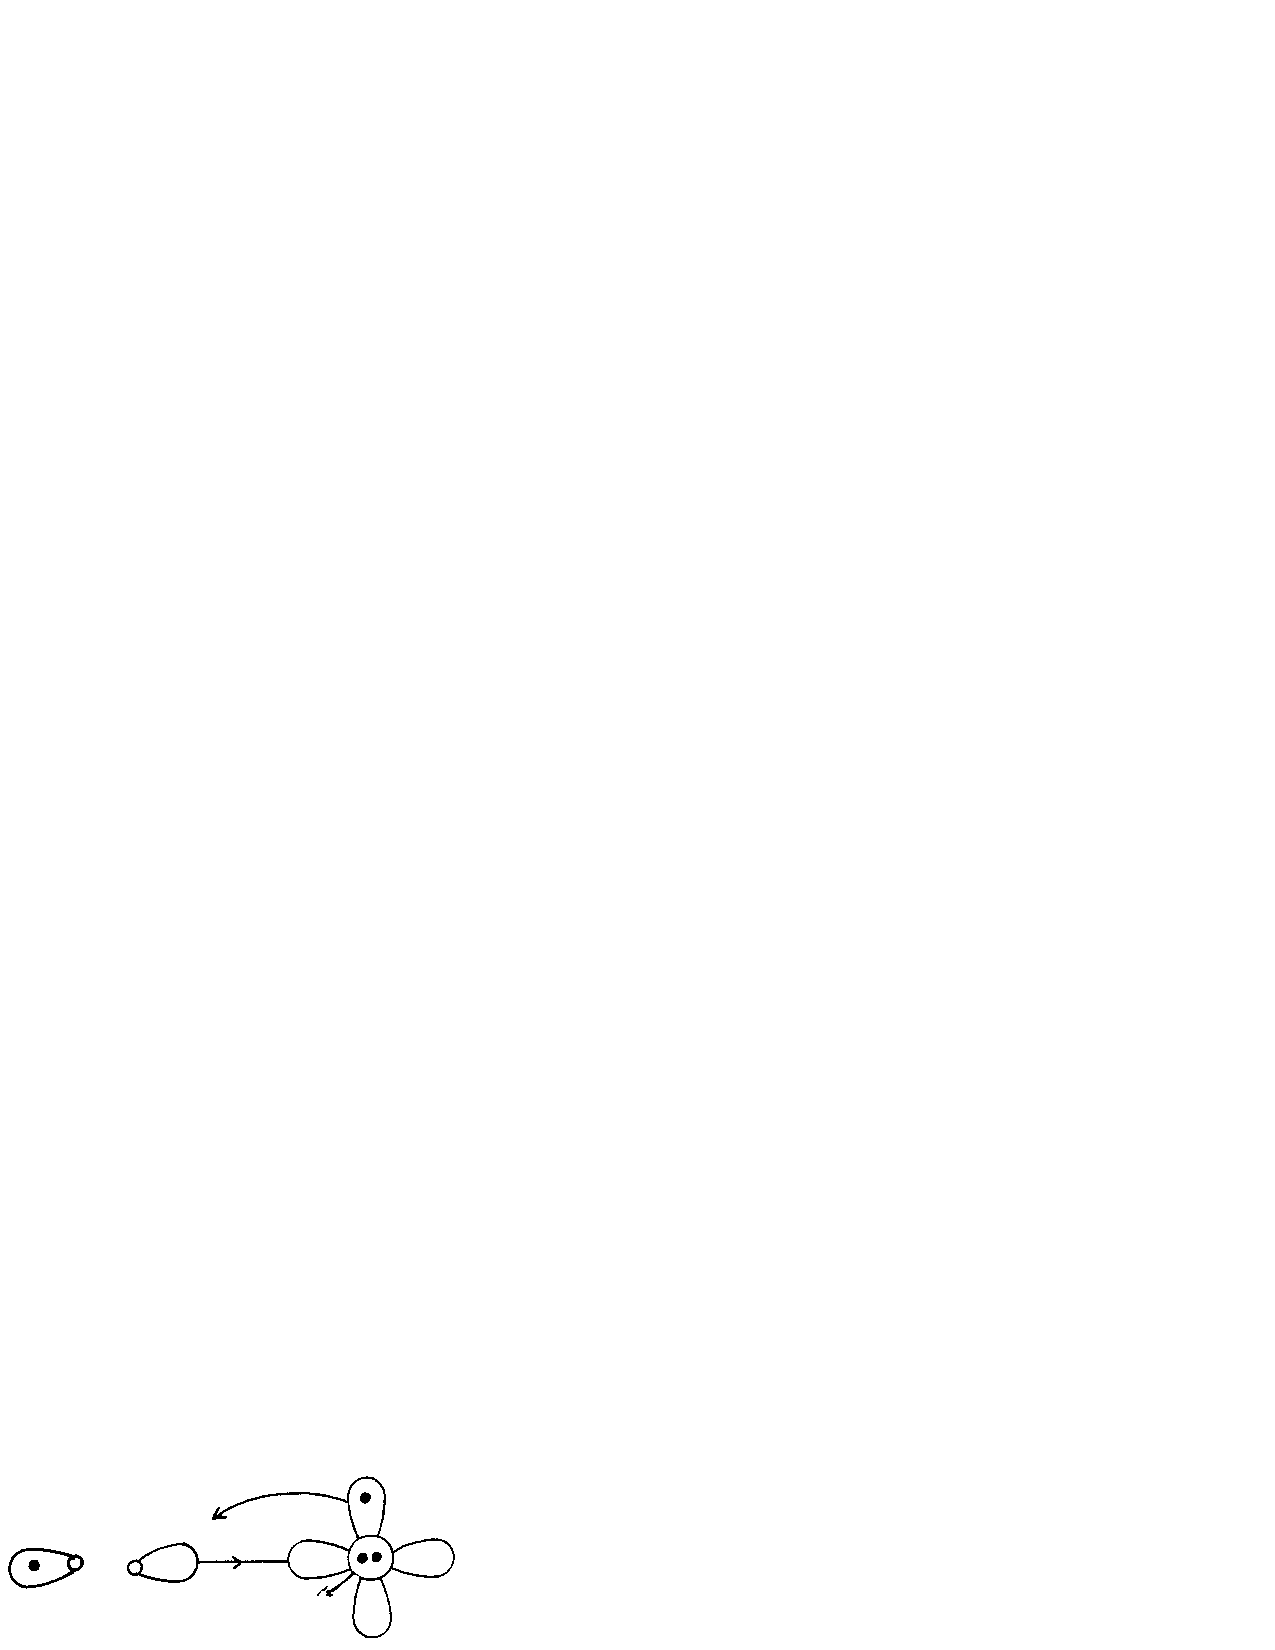
\includegraphics{fg13a}
\label{chap13-eqno1}
\end{equation}
where the arrows indicate that the sigma bond should be ionic toward
the O but the singly occupied pi orbital, on the O, should be strongly
bonding to the Be, and the doubly occupied pi pair on the O should be
somewhat bonding to the Be.  Configuration (\ref{chap13-eqno1}) leads
to ${^3\Pi}$ and ${^1\Pi}$ states of which ${^3\Pi}$ should be lower.

Exciting the nonbonding Be sigma orbital of (\ref{chap13-eqno1}) to be
Be pi orbital, leads to
\begin{equation}
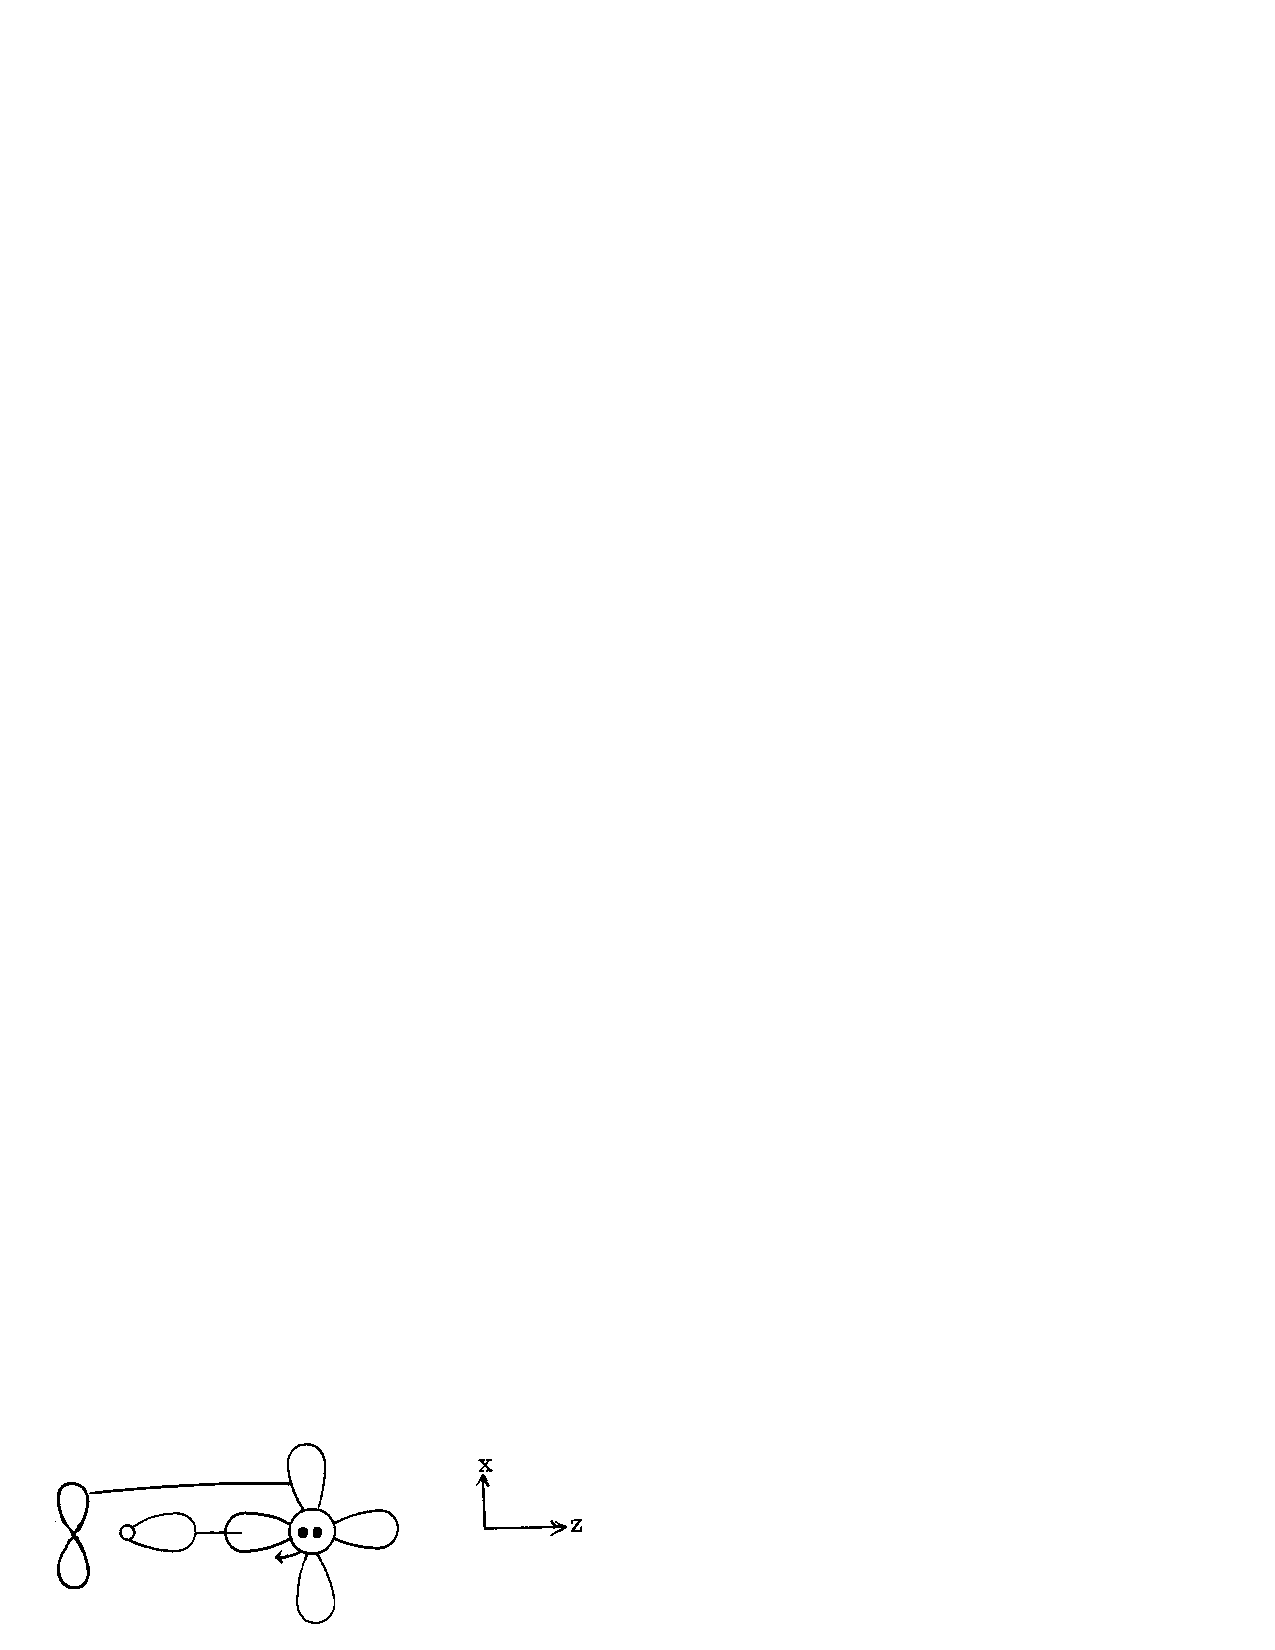
\includegraphics{fg13b}
\label{chap13-eqno2}
\end{equation}
Thus, this leads to a two electron $\pi_x$ bond. In
(\ref{chap13-eqno2}) we have indicated the $\pi_x$ and $\pi_y$ pairs
to be different.  When we actually solve for the orbitals, we find
that the $\pi_x$ and $\pi_y$ pairs become equivalent, having a
character in between the extremes shown in (\ref{chap13-eqno2}) for
the $\pi_x$ and $\pi_y$ pairs.  Thus, the state (\ref{chap13-eqno2})
leads to ${^1\Sigma}^+$ symmetry.

Because of the extra bonding in (\ref{chap13-eqno2}), the
${^1\Sigma}^+_g$ state might be as low as the ${^3\Pi}$ state from
(\ref{chap13-eqno1}).  Indeed, indications are that the ${^1\Sigma}^+$
state is lower.  The experimental results are indicated in Table
\ref{chap13-tab1}.

\begin{table}
\caption{Experimental spectrum of BeO.}
\label{chap13-tab1}
\begin{tabular}{cccccc}\\ \hline
& $T_e$ & $r_e$ & $\omega_e$ &\multicolumn{2}{c}{$D^0_o$}\cr
& (cm$^{-1}$) & (\AA) & (cm$^{-1}$) & (cm$^{-1}$) & (kcal)\cr

X$^1\Sigma$ & 0 & 1.3310 & 1487.32 & 37100 $\pm$ 800 & 106.1\cr
$^1\Pi$ & 9405.5 & 1.4632 & 1144.24\cr
$^1\Sigma$ & 21253.95 & 1.3623 & 1370.82\cr
D & 39120.1 & 1.49 & 1081.5\cr
\hline
\end{tabular}
\end{table}

Figures \ref{chap13-fig1} and \ref{chap13-fig2} show the generalized
valence bond orbitals for the ${^1\Sigma}^+$ and ${^3\Pi}$ states of
BeO.
\begin{figure}
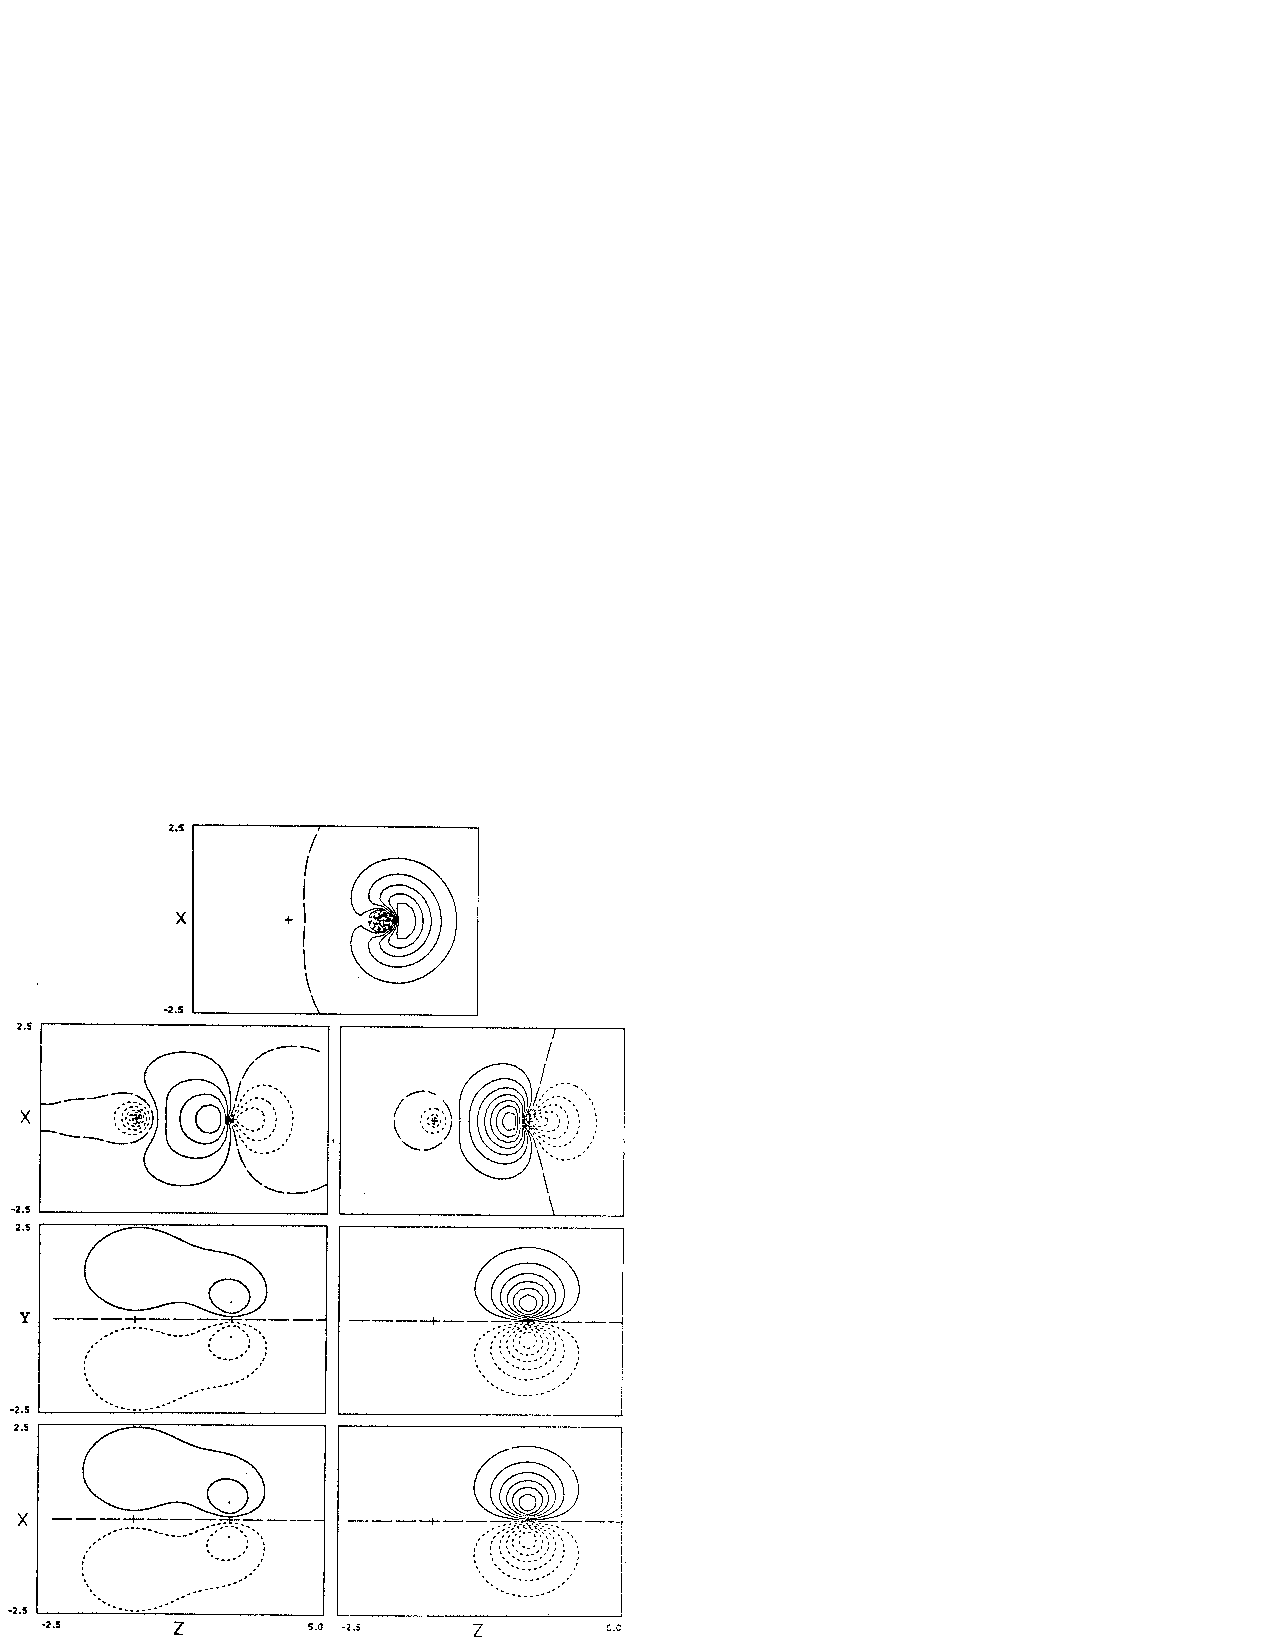
\includegraphics[scale=0.75]{fg13-1}
\caption{GVB orbitals of the $^1E^+$  state of BeO, 
configuration (\ref{chap13-eqno1}).  The first row contains the O2s
orbital, doubly occupied, the second row is the sigma bonding pair,
and the other two rows the pi pairs.  }
\label{chap13-fig1}
\end{figure}

\begin{figure}
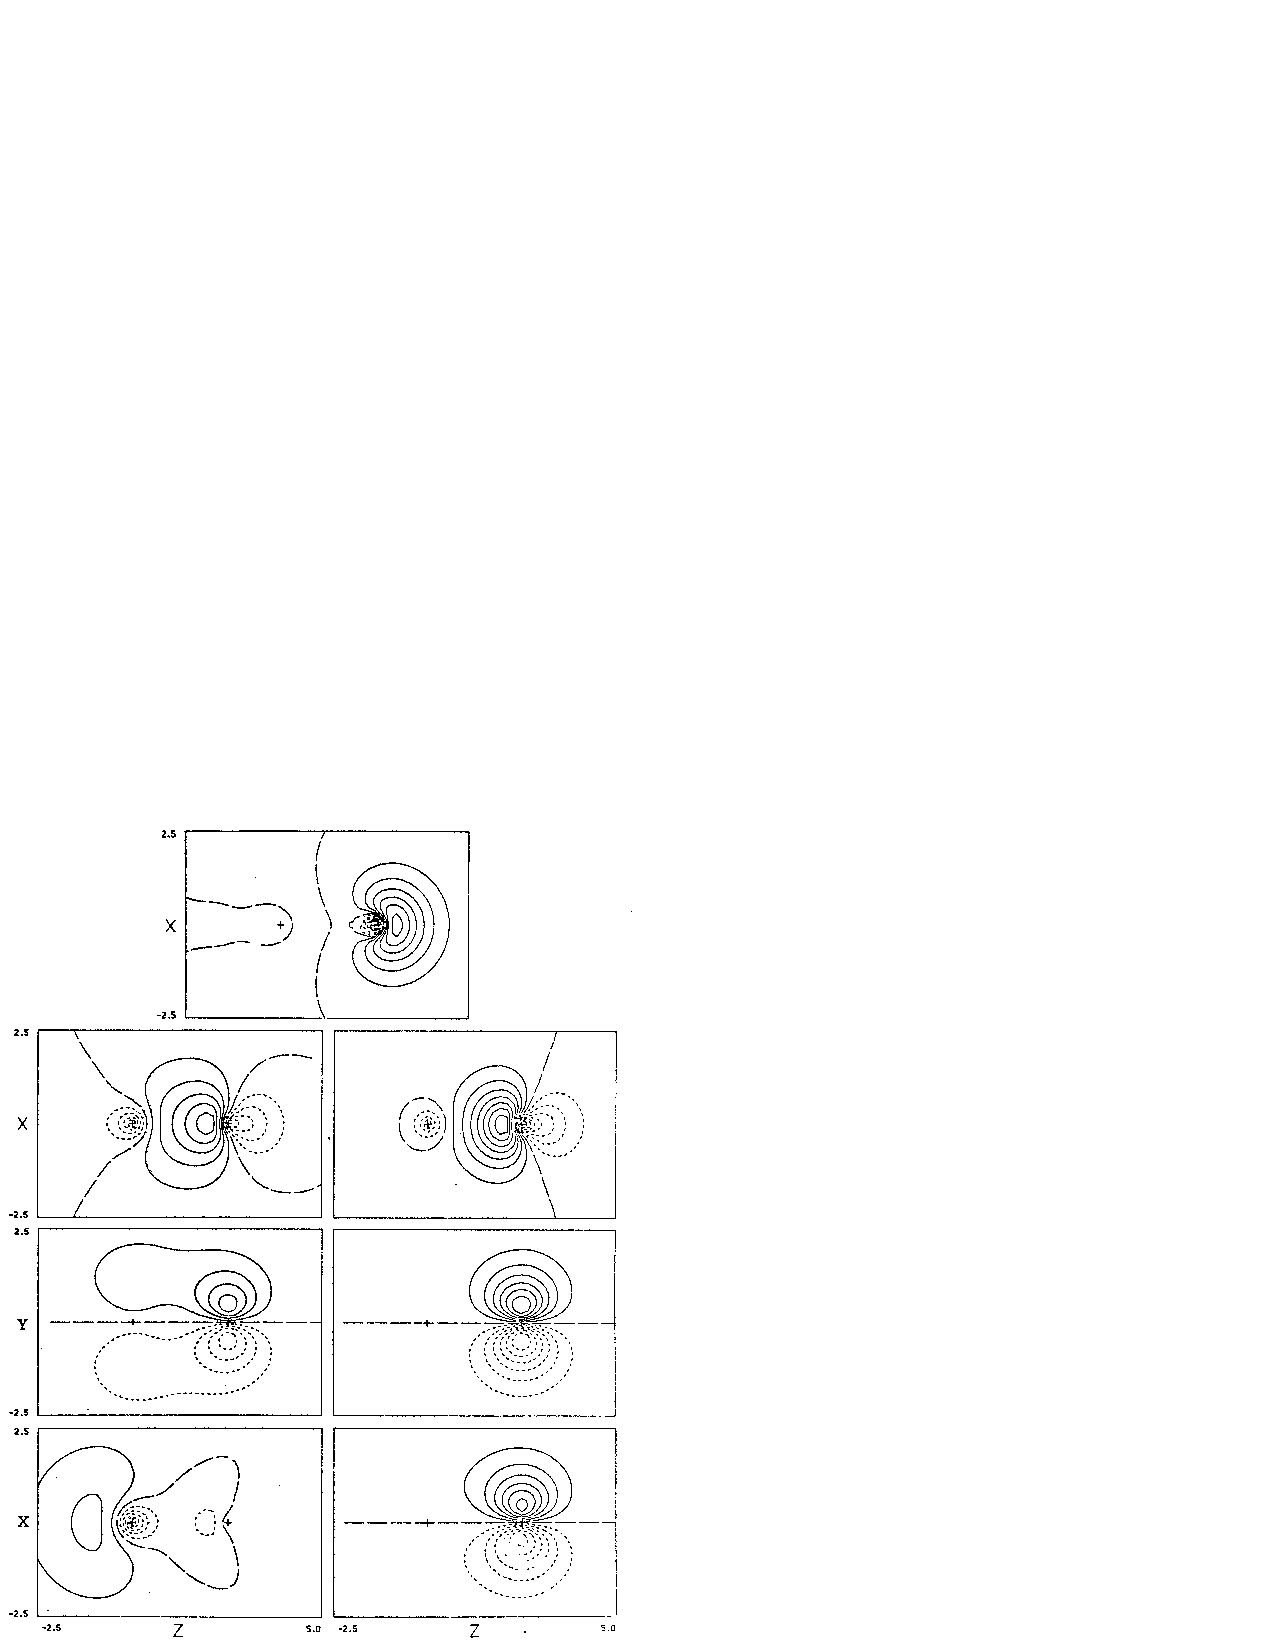
\includegraphics[scale=0.75]{fg13-2}
\caption{GVB orbitals of the ${^3\Pi}$ state of BeO, configuration
(\ref{chap13-eqno2}).} 
\label{chap13-fig2}
\end{figure}

\begin{table}
\caption{BeO with pair information.}
\label{chap13-tab2}
\begin{tabular}{ccccc}\\ \hline

& Energy & Pair & $\Delta$E & S$_{a,b}$\cr

$^1\Sigma^+$ & $-$88.9046 & b & .0085 & .8618\cr
& & $\pi_x$ & .0312 & .6662\cr
& & $\pi_y$ & .0312 & .6662\cr
$^3\Pi$ & $-$88.8994 & b & .0046 & .9117\cr
& & $\pi_y$ & .0120 & .8090\cr
$^1\Pi$ & $-$88.8914 & b & .0048 & .9094\cr
& & $\pi_y$ & .0131 & .7995\cr
$^3\Sigma^+$ & $-$88.8759 & b & .0014 & .9587\cr
& & $\pi_x$ & .0079 & .8495\cr
& & $\pi_y$ & .0079 & .8495\cr
$^3\Sigma^-$ & $-$88.7201 & b & .0023 & .9431\cr
& & $\pi$ & .0187 & .6138\cr
$^3\Sigma^-$ & $-$88.6757 & b & .0089 & .855\cr
& & O2s & .0009 & .9803\cr

\hline
\end{tabular}
\end{table}

Some data about these states are also included in Table
\ref{chap13-tab2}.  The ${^3\Sigma}^+$ state is obtained from the
configurations
\begin{equation}
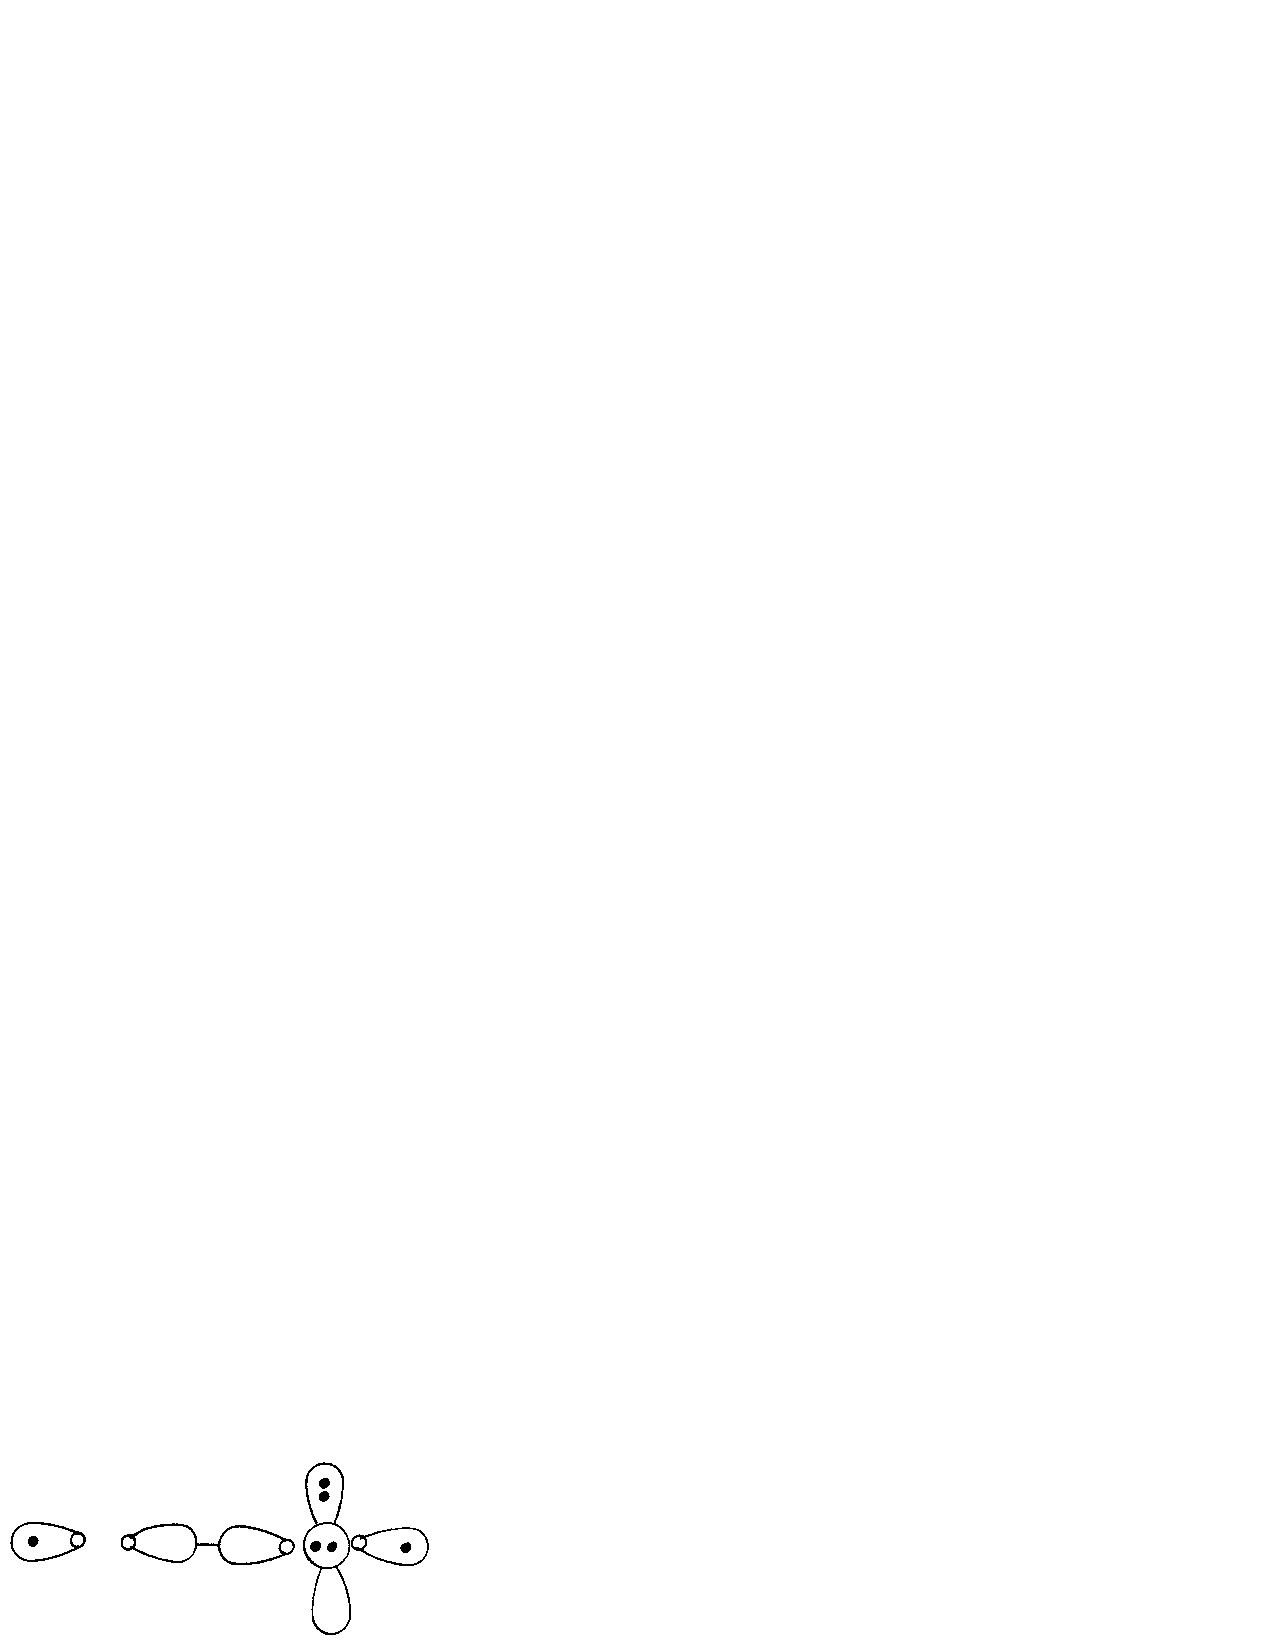
\includegraphics{fg13-2a}
\end{equation}
where we have split the 2s pair of O.  This state and
(\ref{chap13-eqno1}) are both limits of the configuration
\begin{equation}
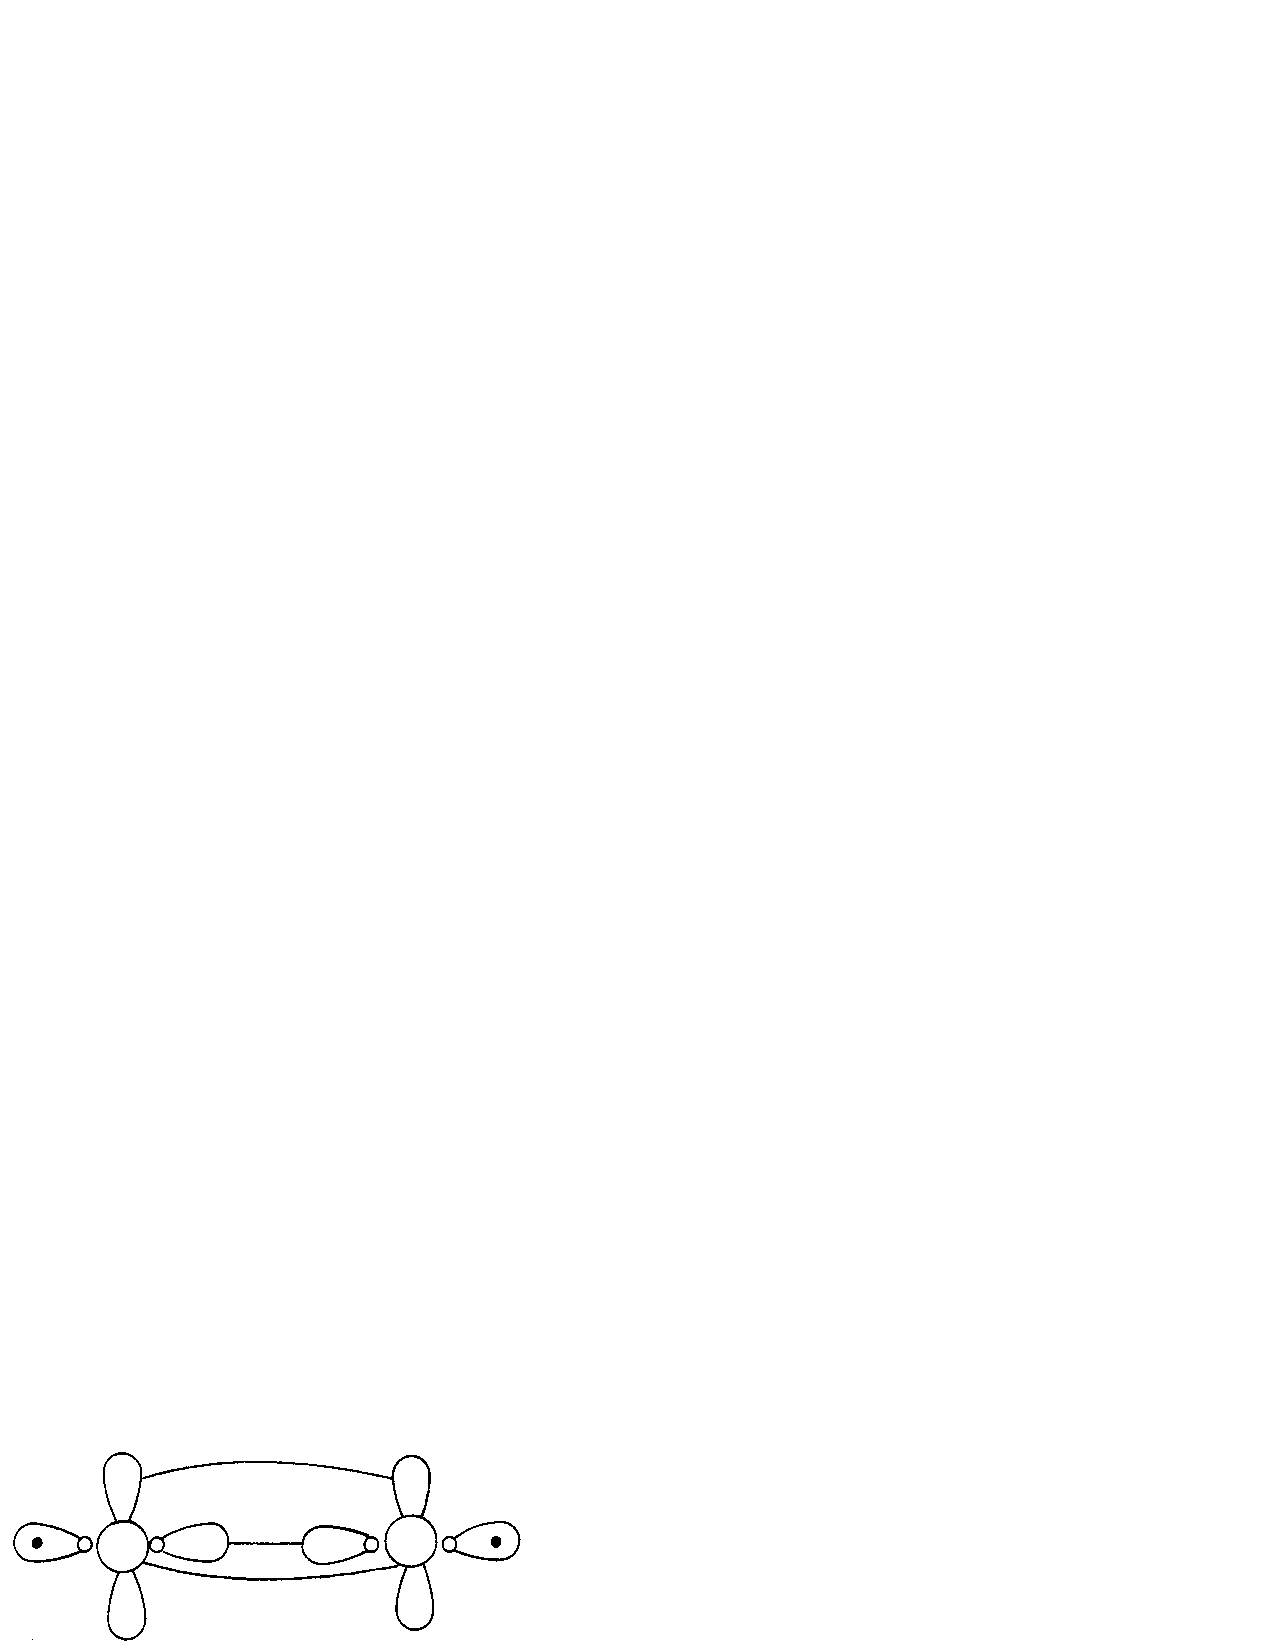
\includegraphics{fg13-2b}
\end{equation}
of C$_2$.

The two ${^3\Sigma}^-$ states of BeO arise from the configurations
\begin{equation}
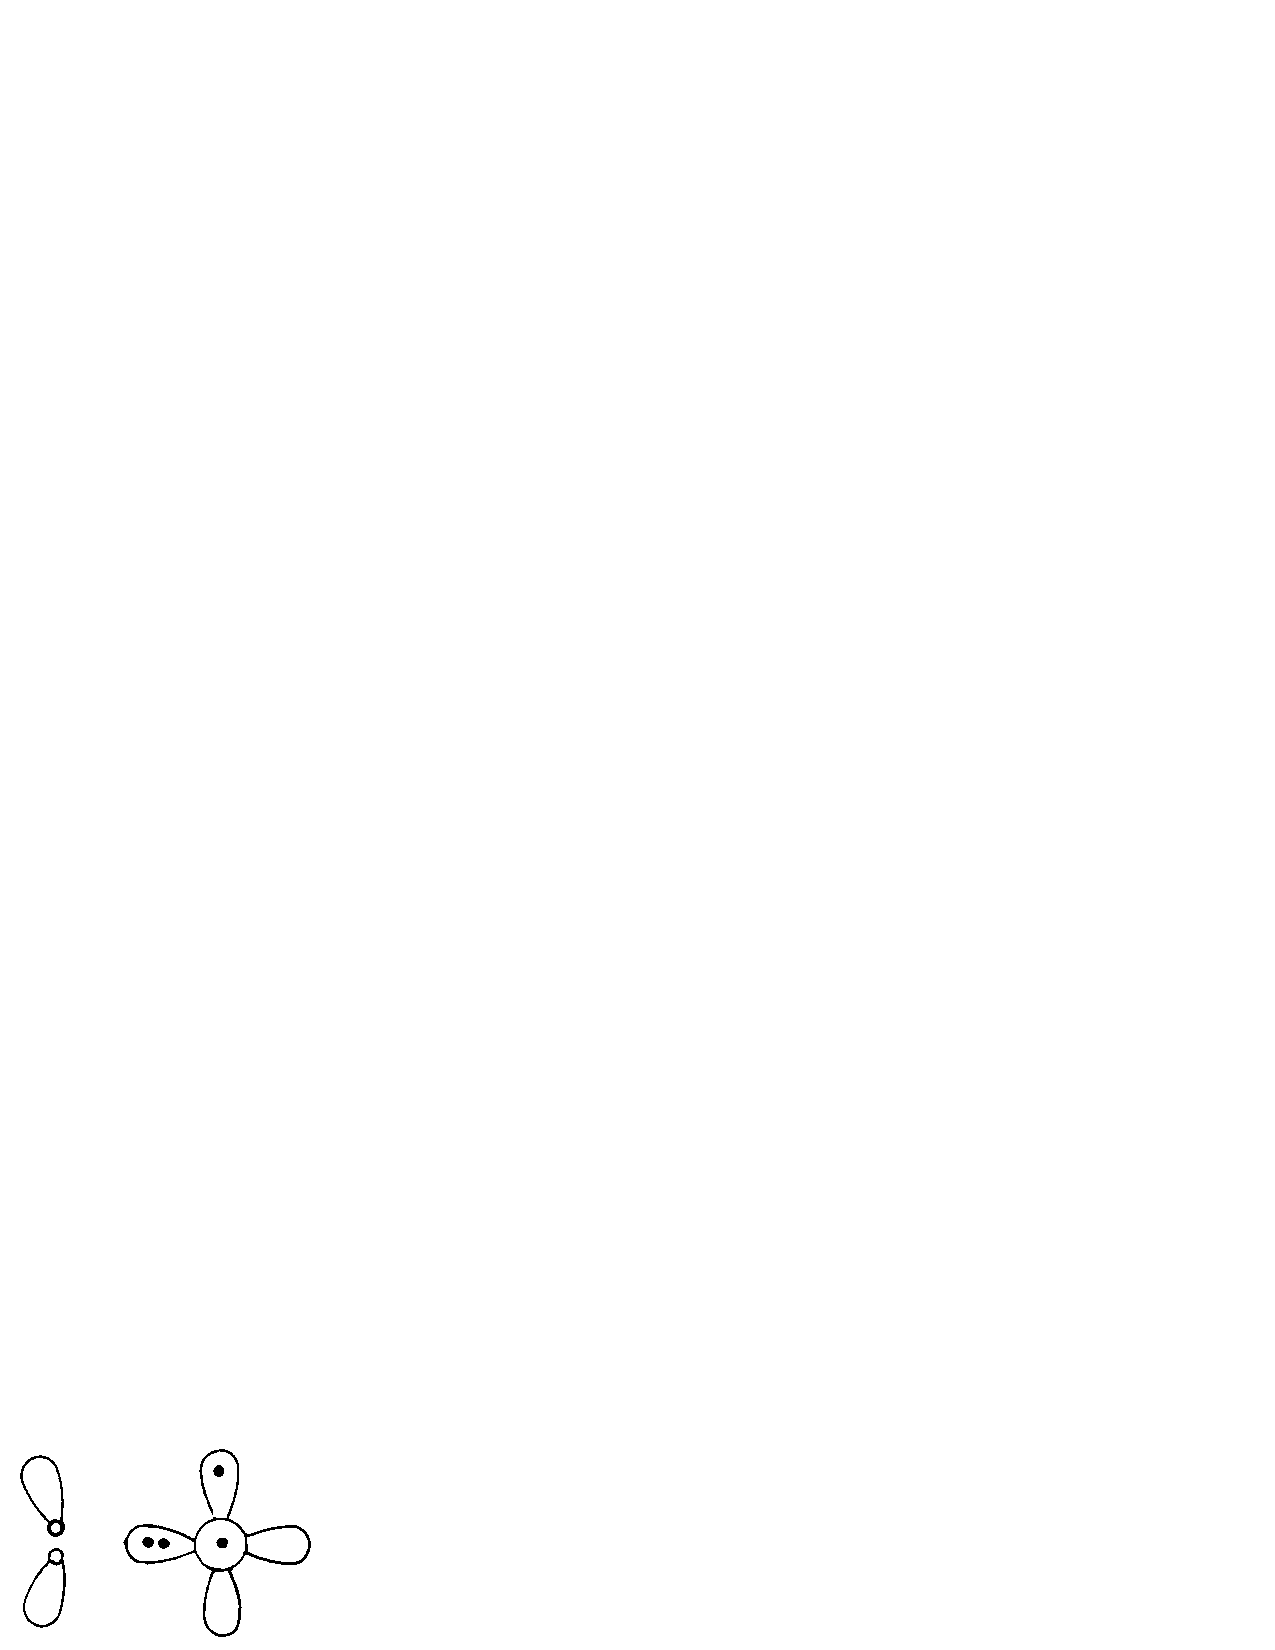
\includegraphics{fg13-2c}
\end{equation}
and
\begin{equation}
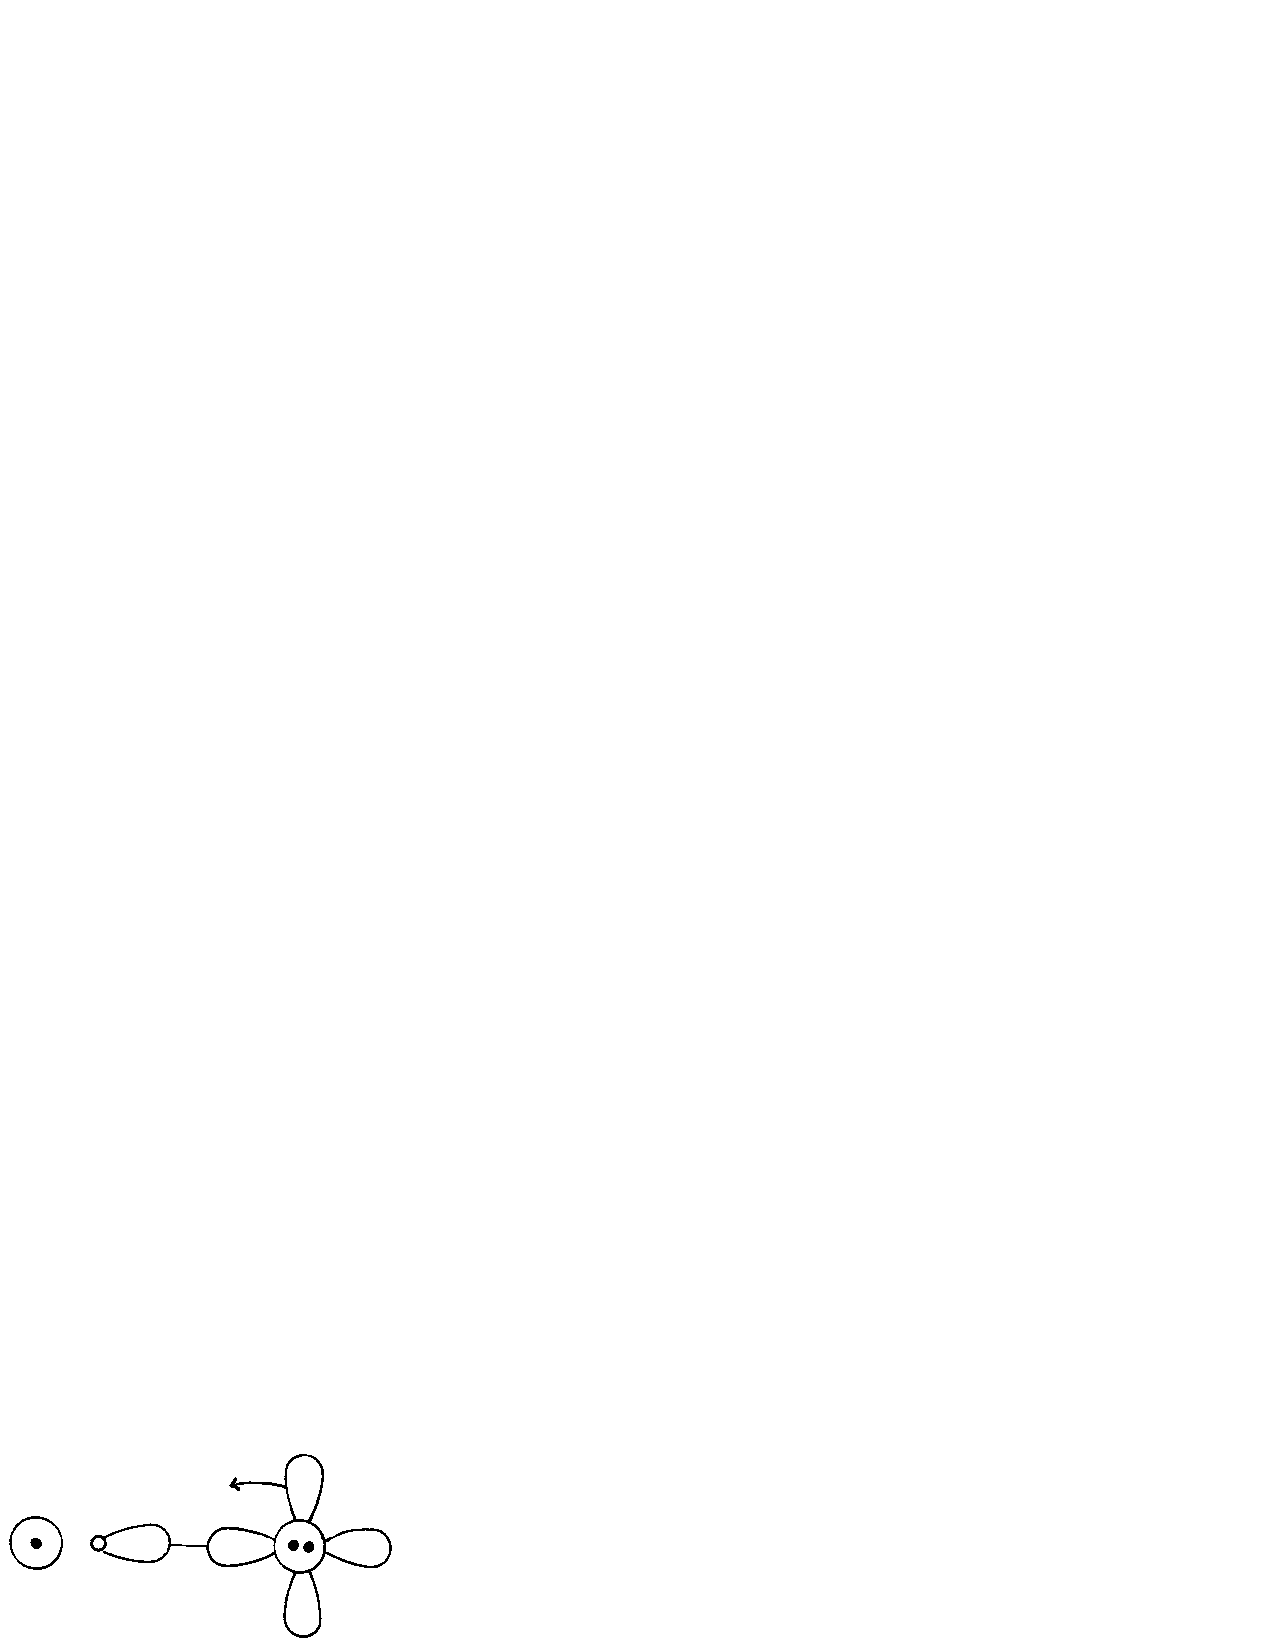
\includegraphics{fg13-2d}
\label{chap13-eqno3}
\end{equation}
respectively.

Adding a second O to BeO, BeO$_2$, should lead to linear states with a
${^3\Sigma}^-_g$ state
\begin{equation}
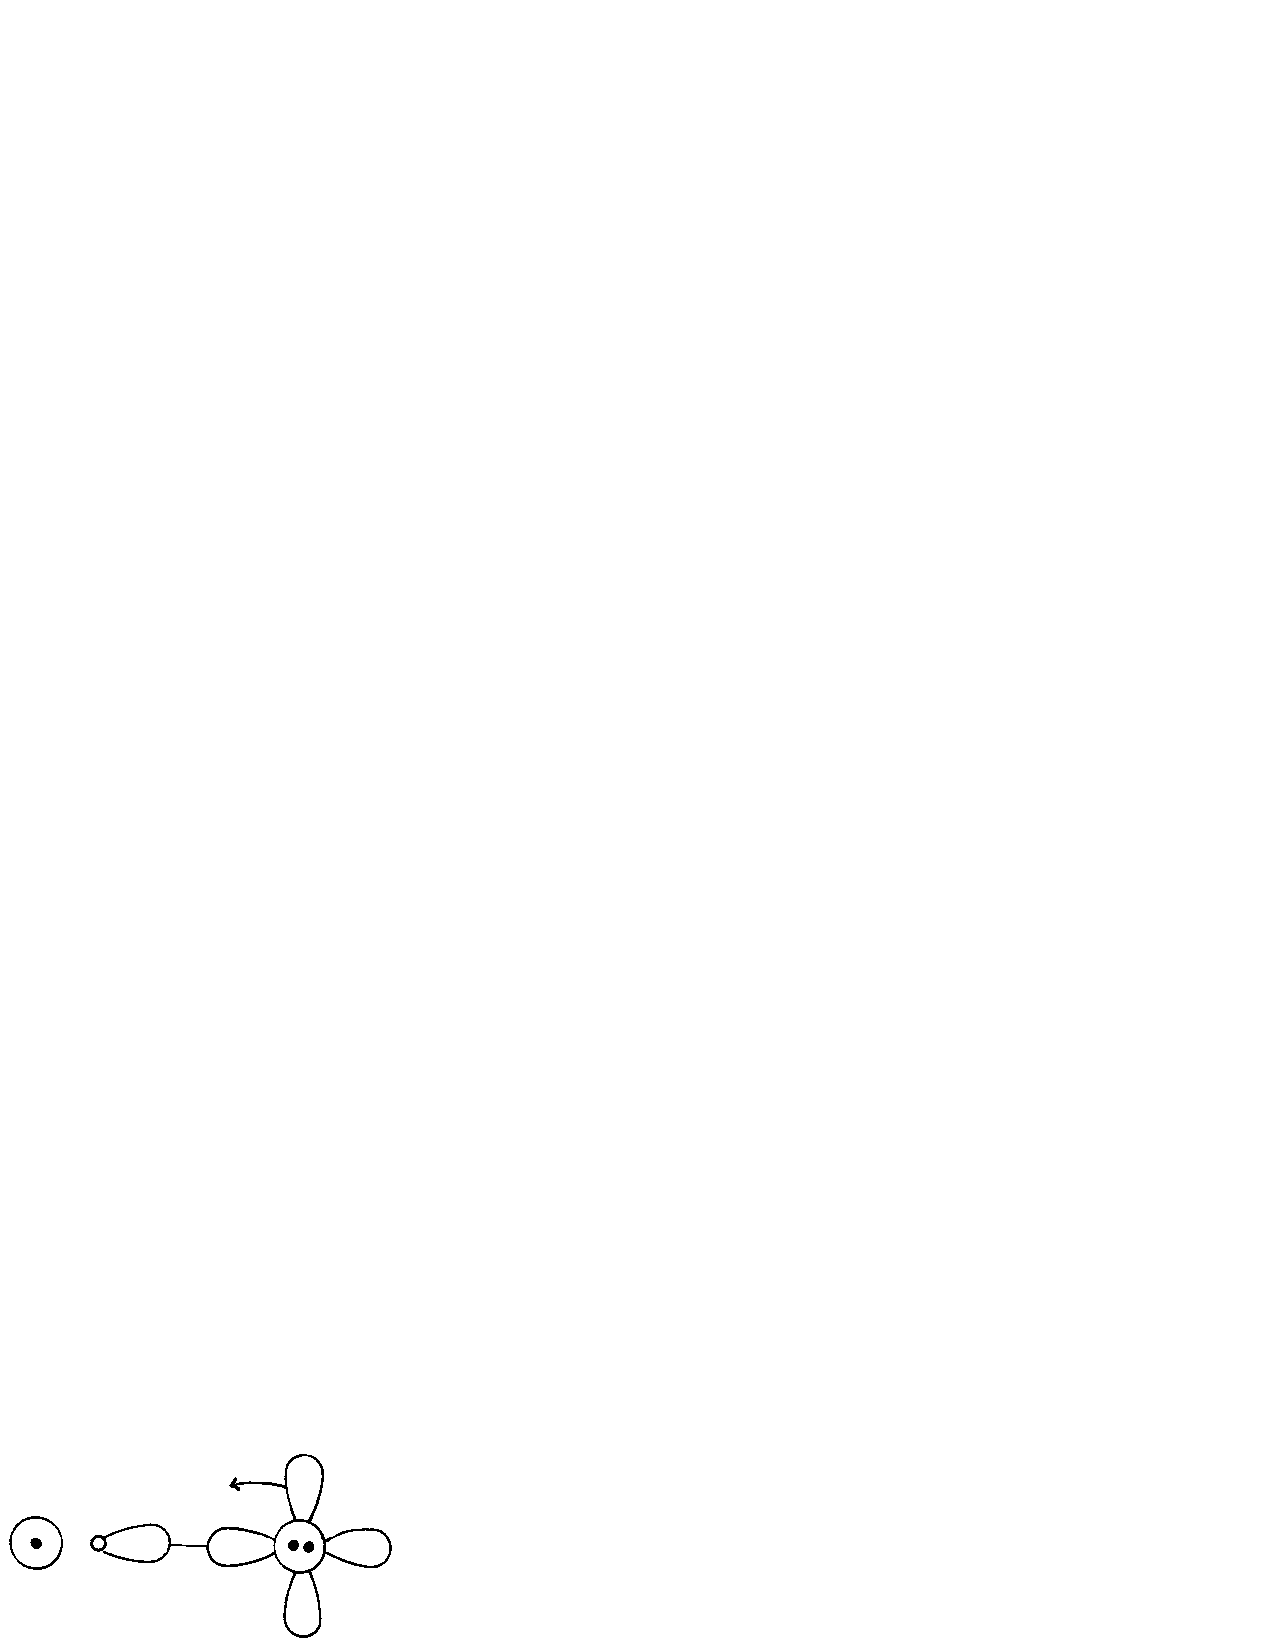
\includegraphics{fg13-2d}
\end{equation}
and corresponding higher ${^1\Delta}_g$ and ${^1\Sigma}^+_g$ states.

\section{BO}

From the ground states of B and O, we obtain
\begin{equation}
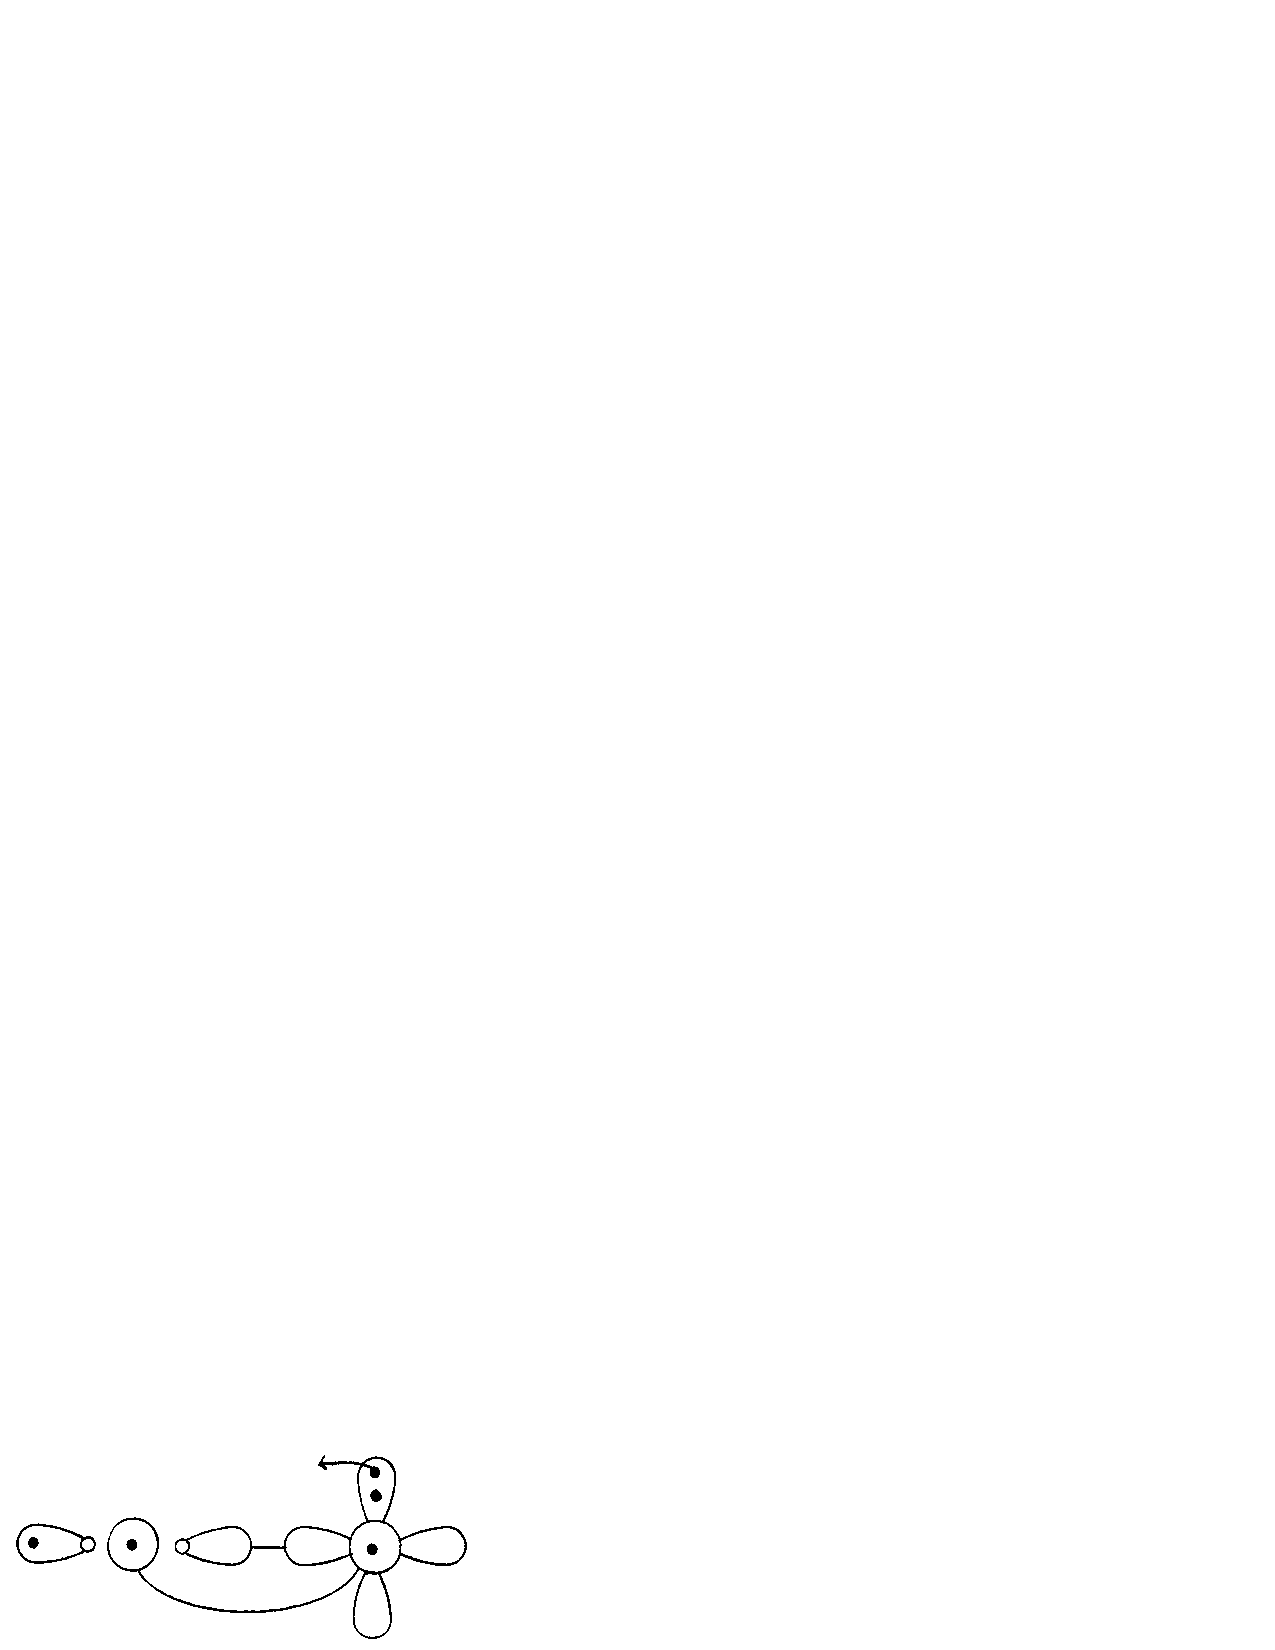
\includegraphics{fg13-2f}
\label{chap13-eqno4}
\end{equation}
leading to a ${^2\Sigma}^+$ state, the pi pairs become equivalent.  An 
excited ${^2\Pi}$ state is obtained from
\begin{equation}
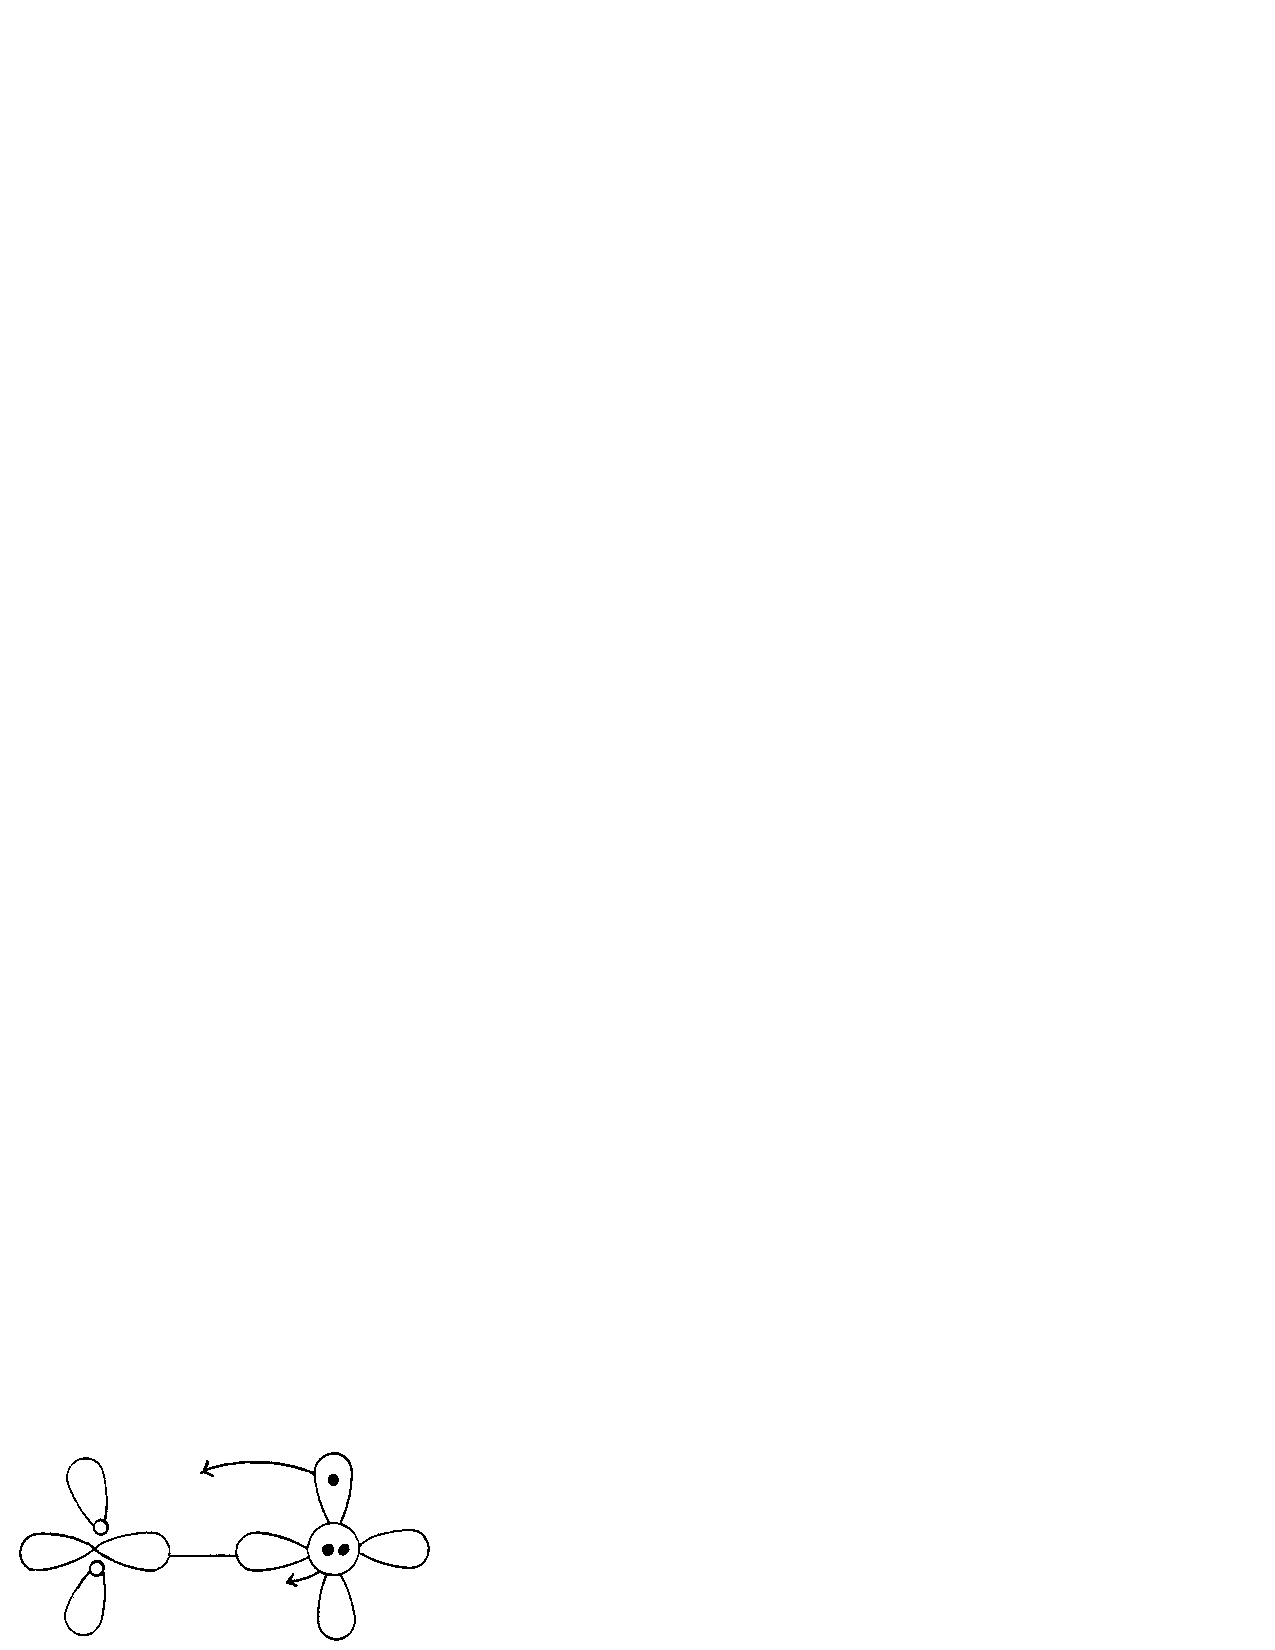
\includegraphics{fg13-2g}
\label{chap13-eqno5}
\end{equation}
Starting from the ${^1S}$ state of O, we can also form the 
${^2\Sigma}^+$ state
\begin{equation}
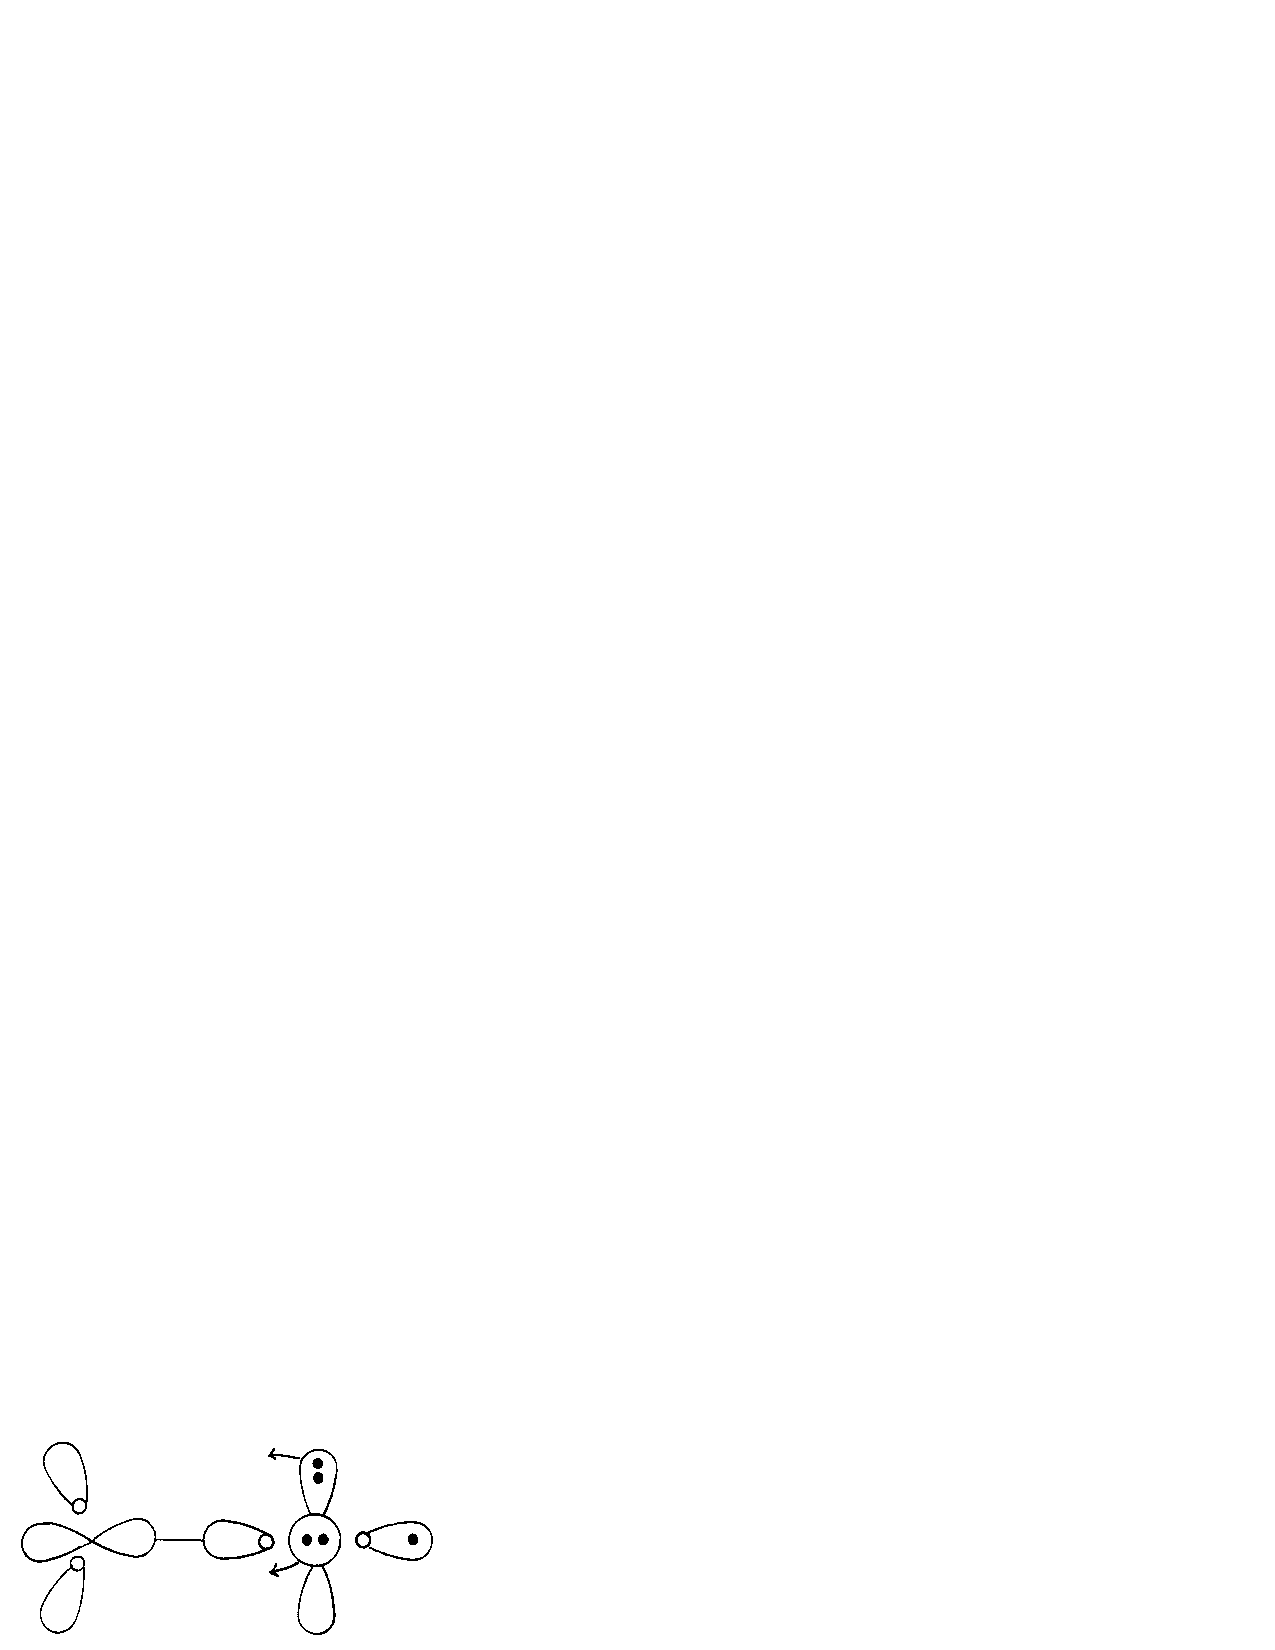
\includegraphics{fg13-2h}
\label{chap13-eqno6}
\end{equation}
and the ${^2\Pi}$ state
\begin{equation}
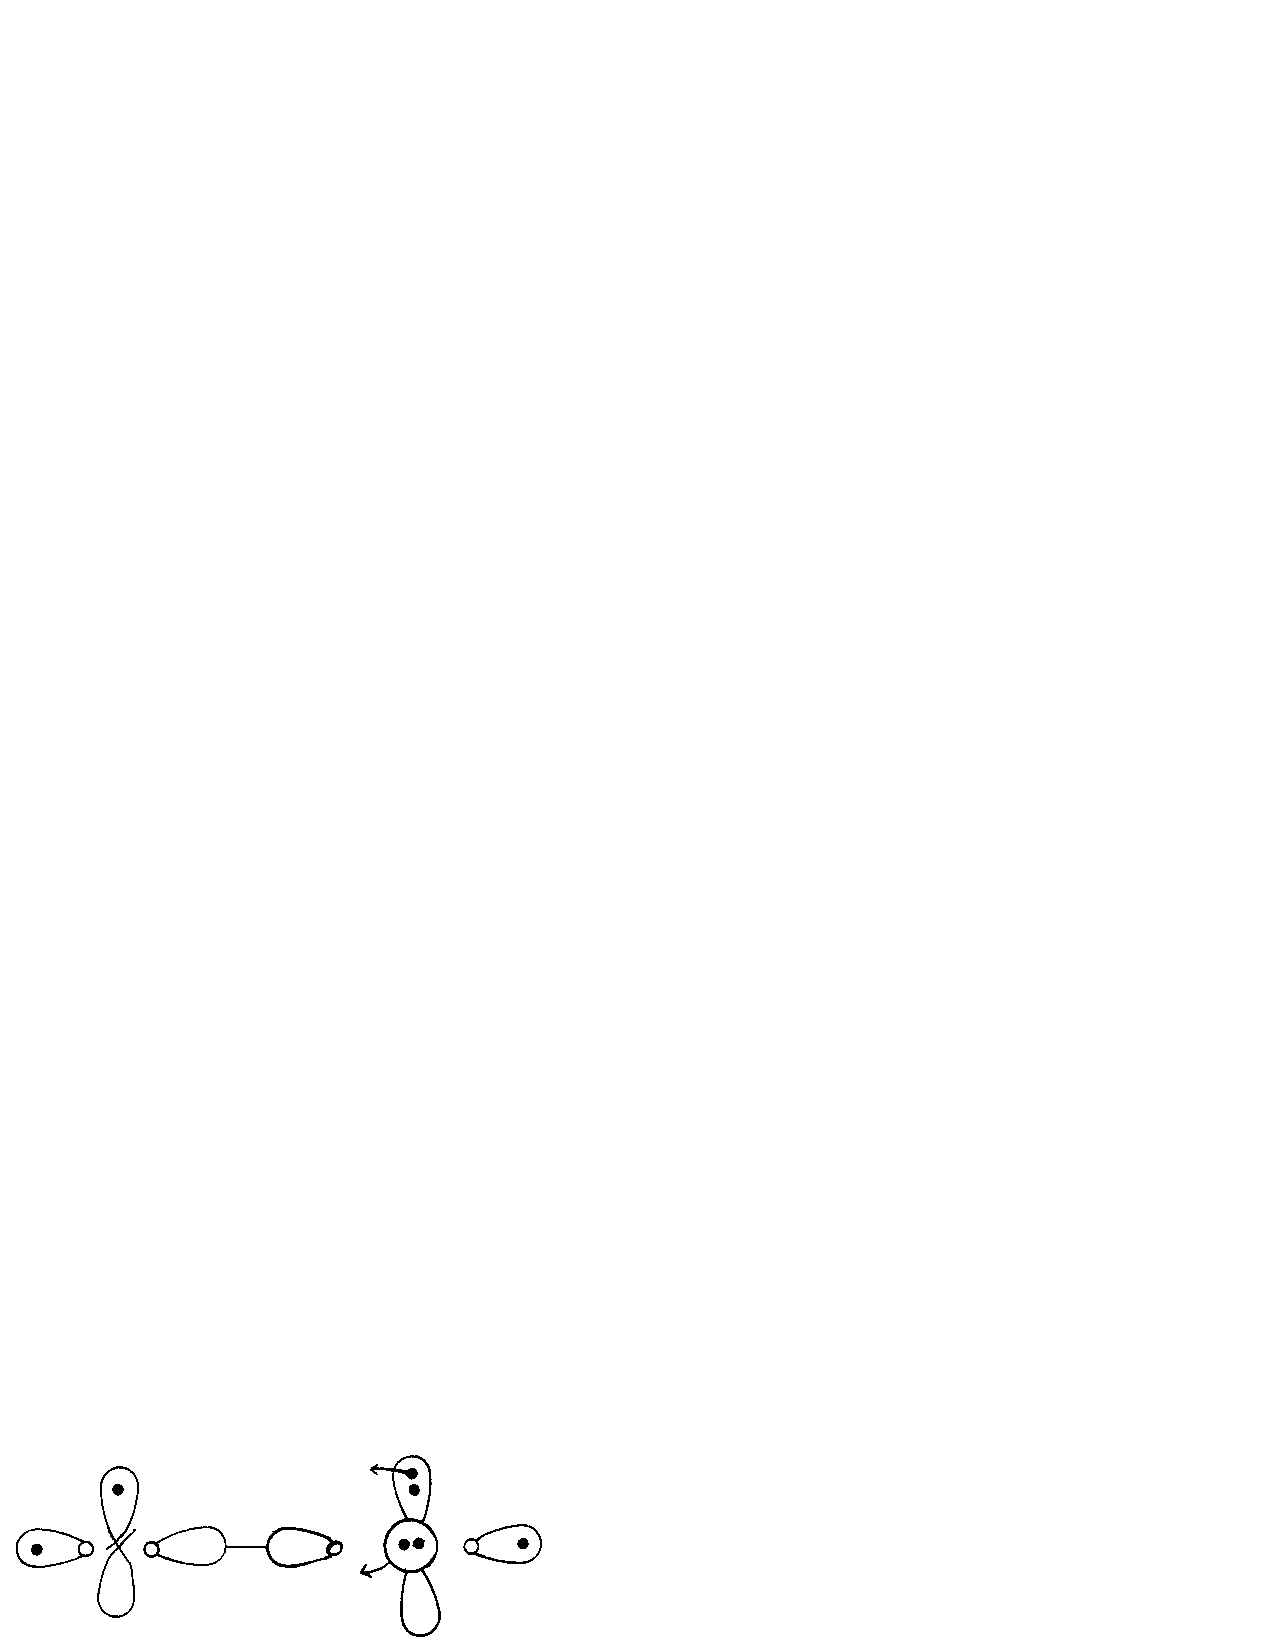
\includegraphics{fg13-2i}
\label{chap13-eqno7}
\end{equation}
singlet coupling of the $\phi_{\sigma L}$ and $\phi_{\sigma R}$
orbitals, we can also obtained a ${^4\Pi}$ state.  The experimental
results are in Tables \ref{chap13-tab3a}--\ref{chap13-tab3b}.

\begin{table}
\caption{Experimental results for BO.}
\label{chap13-tab3a}
\begin{tabular}{cccccc}\\ \hline

& $T_e$ & $r_e$ & $\omega_e$ &\multicolumn{2}{c}{$D^0_o$}\cr
& (cm$^{-1}$) & (\AA) & (cm$^{-1}$) & (cm$^{-1}$) & (kcal)\cr

X $^2\Sigma^+$ & 0 & 1.2043 & 1885.69 & 66870 $\pm$ 800 & 191.2\cr
A $^2\Pi$ & 23959 & 1.3524 & 1260.70\cr
& 23836 & 1.3524 & 1260.70\cr
B $^2\Sigma^+$ & 43174.0 & 1.3053 & 1281.69\cr
C $^2\Pi$ & 55346.1 & 1.3196 & 1315.3\cr

\hline
\end{tabular}
\end{table}

\begin{table}
\caption{Experimental results for BO$^+$.}
\label{chap13-tab3b}
\begin{tabular}{cccc}\\ \hline

& $T_o$ & $r_o$ & $\omega_o$\cr
& (cm$^{-1}$) & (\AA) & (cm$^{-1}$)\cr

$^1\Sigma$ & - & 1.199 & 1787\cr
$^1\Sigma$ & 28023.99 & 1.192  & 1952\cr

\hline
\end{tabular}
\end{table}

Of all the states (\ref{chap13-eqno4}) through (\ref{chap13-eqno7}),
the ${^2\Sigma}$ state (\ref{chap13-eqno4}) should have the lowest
energy, the shortest $r$, and the largest $\omega$. The states of
(\ref{chap13-eqno6}) and (\ref{chap13-eqno7}) should be far higher
than (\ref{chap13-eqno5}) since they involve O(${^1S}$).  Of these,
(\ref{chap13-eqno7}) should be higher since it has an antibonding
orbital on the B and it should have a longer $r$. These expectations
are all in agreement with the experimental results. Note that BO$^+$
should also have a ${^1\Pi}$ state about 1 eV above the ground state.

Adding a H to BO, should lead to linear HBO
\begin{equation}
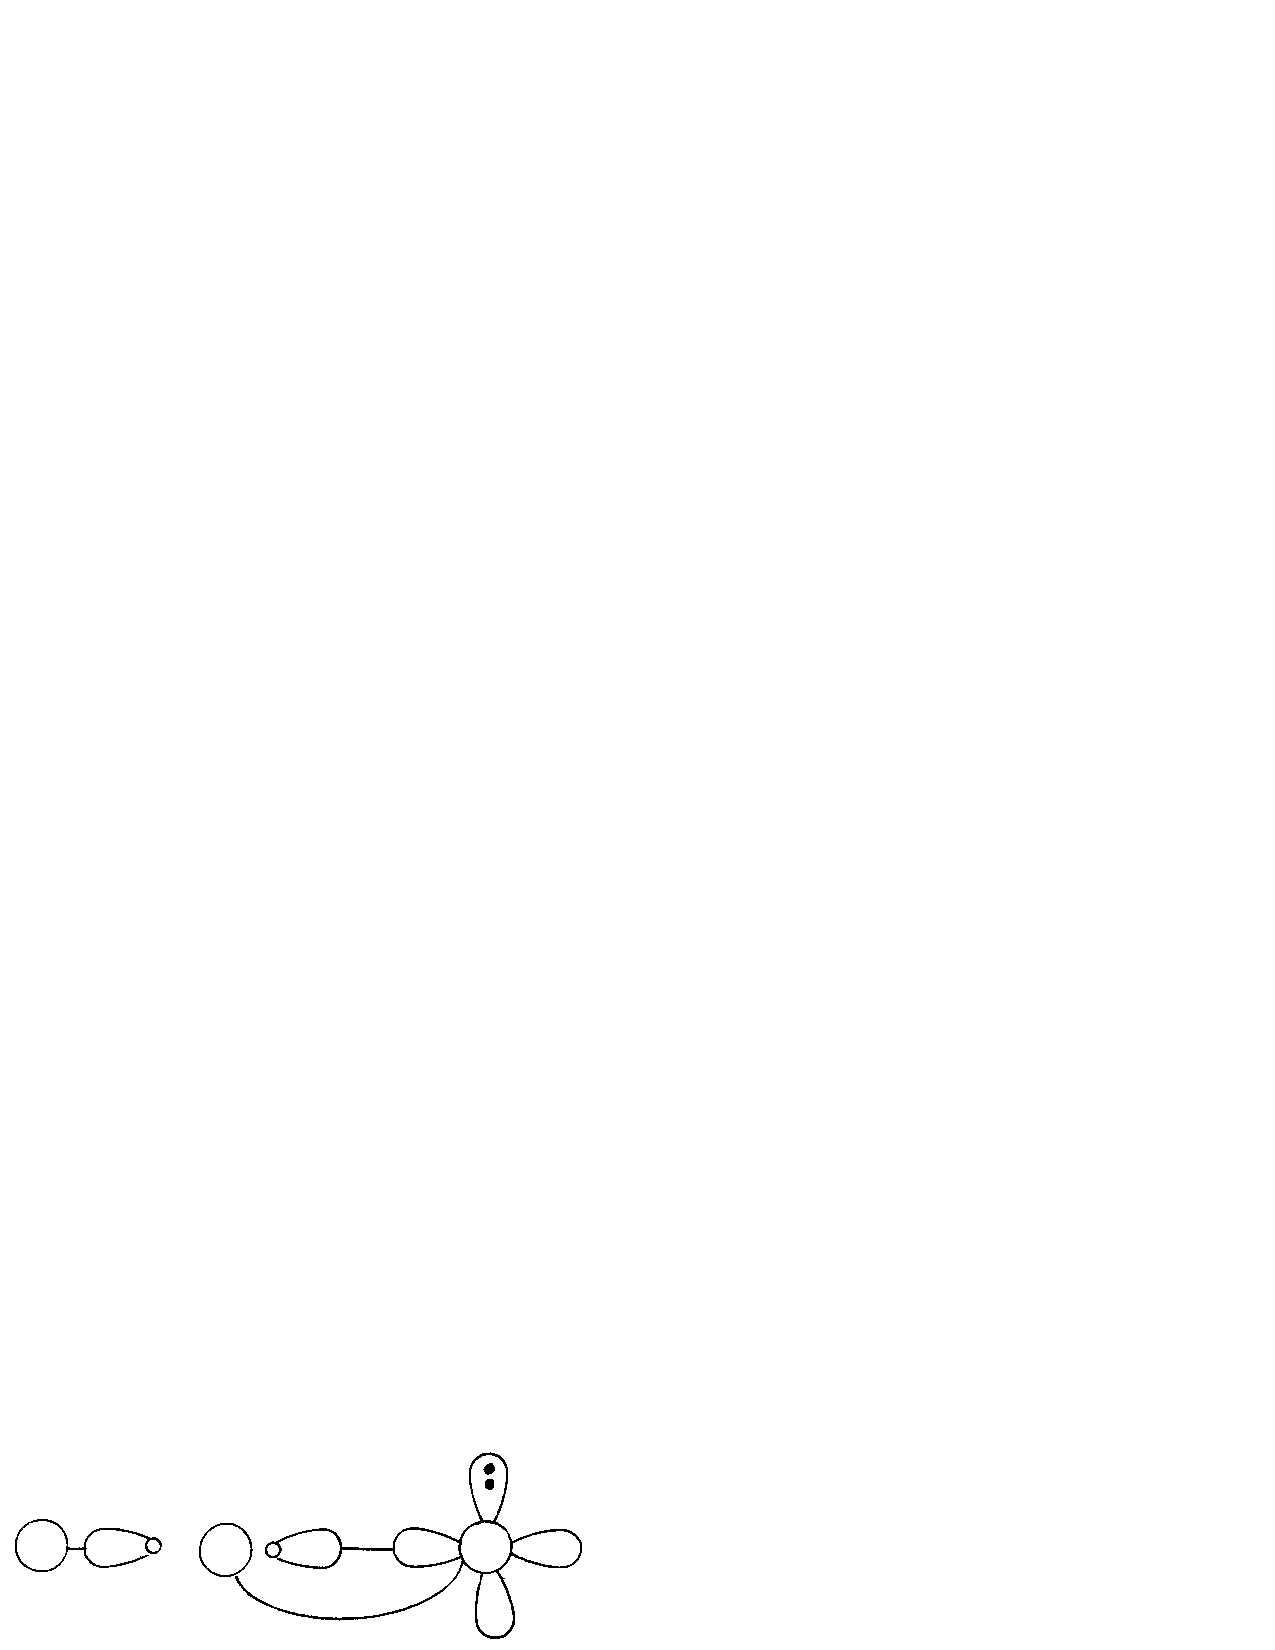
\includegraphics{fg13-2j}
\end{equation}
in a ${^1\Sigma}$ state.

Adding a second O to BO, leads to a linear molecular
\begin{equation}
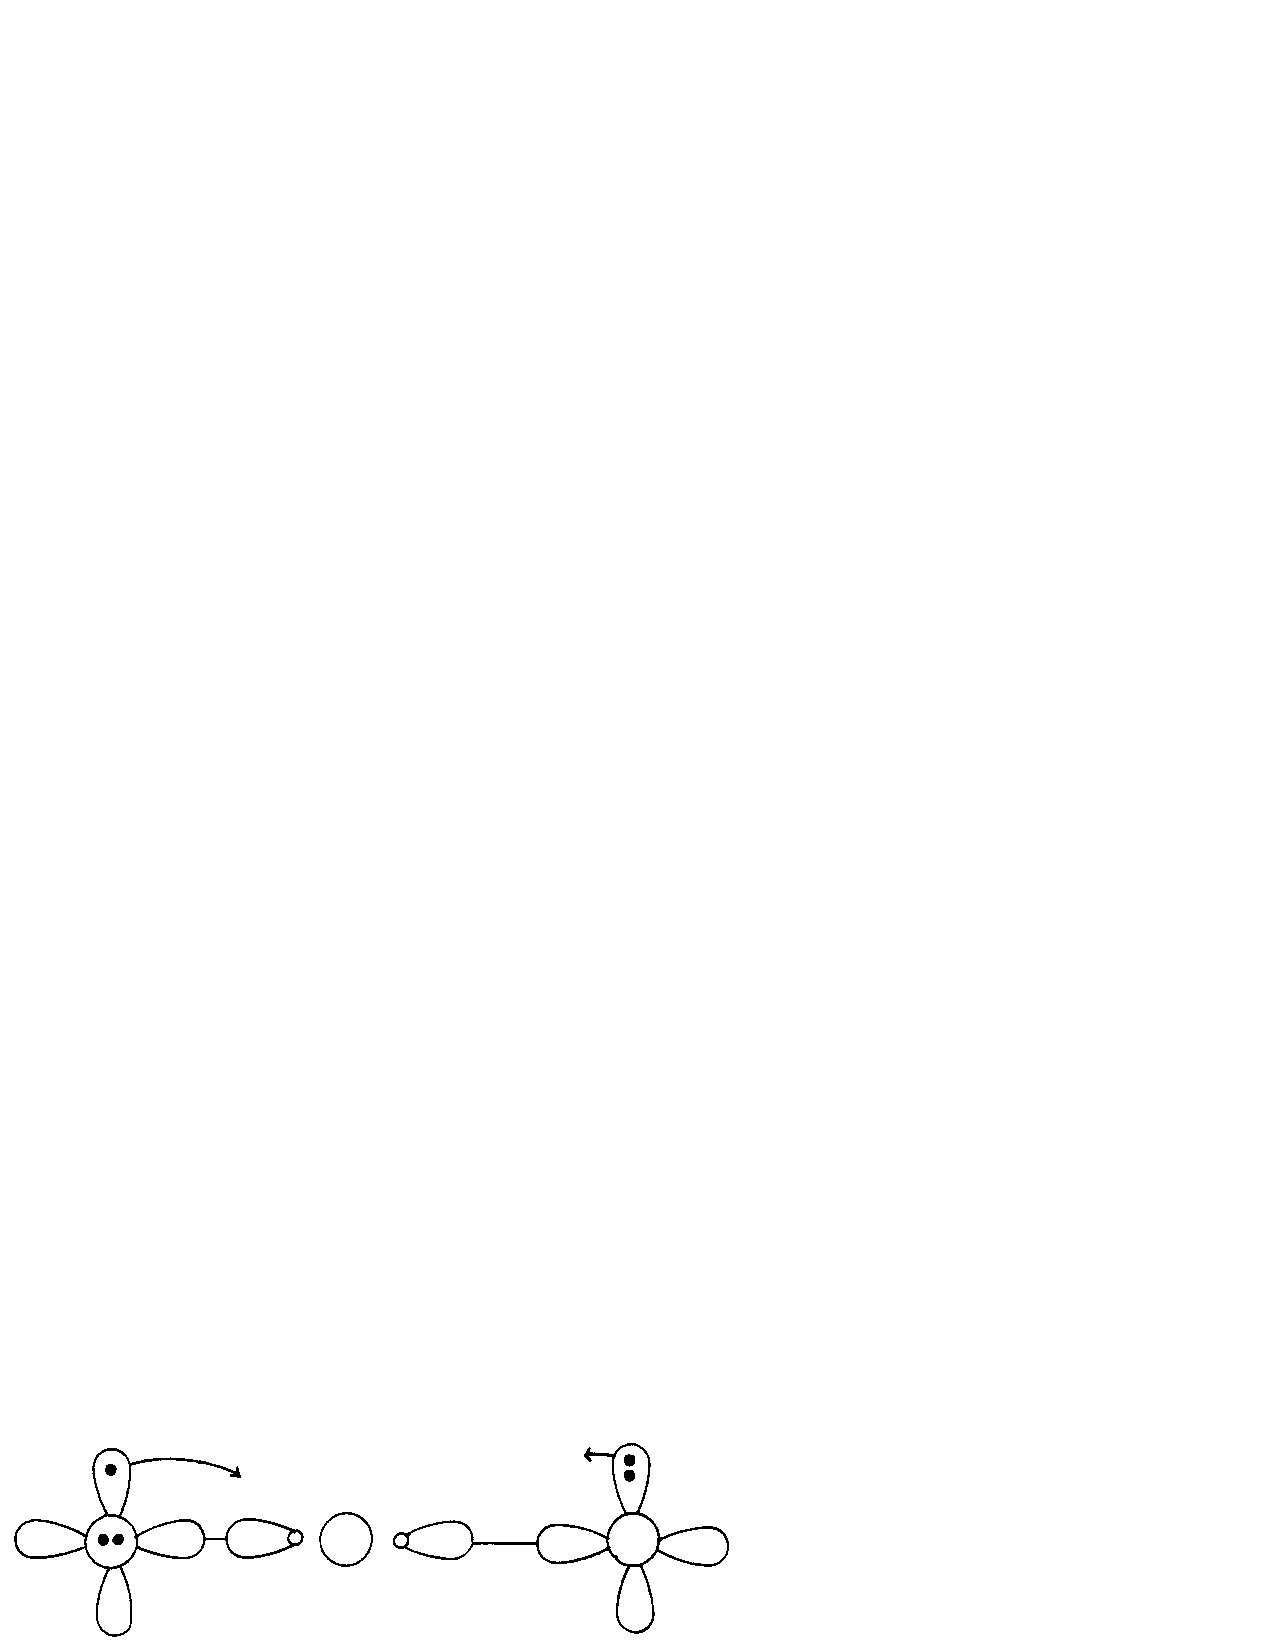
\includegraphics{fg13-2k}
\end{equation}

\section{CO}

Starting with the ground states of C and O, we obtain
\begin{equation}
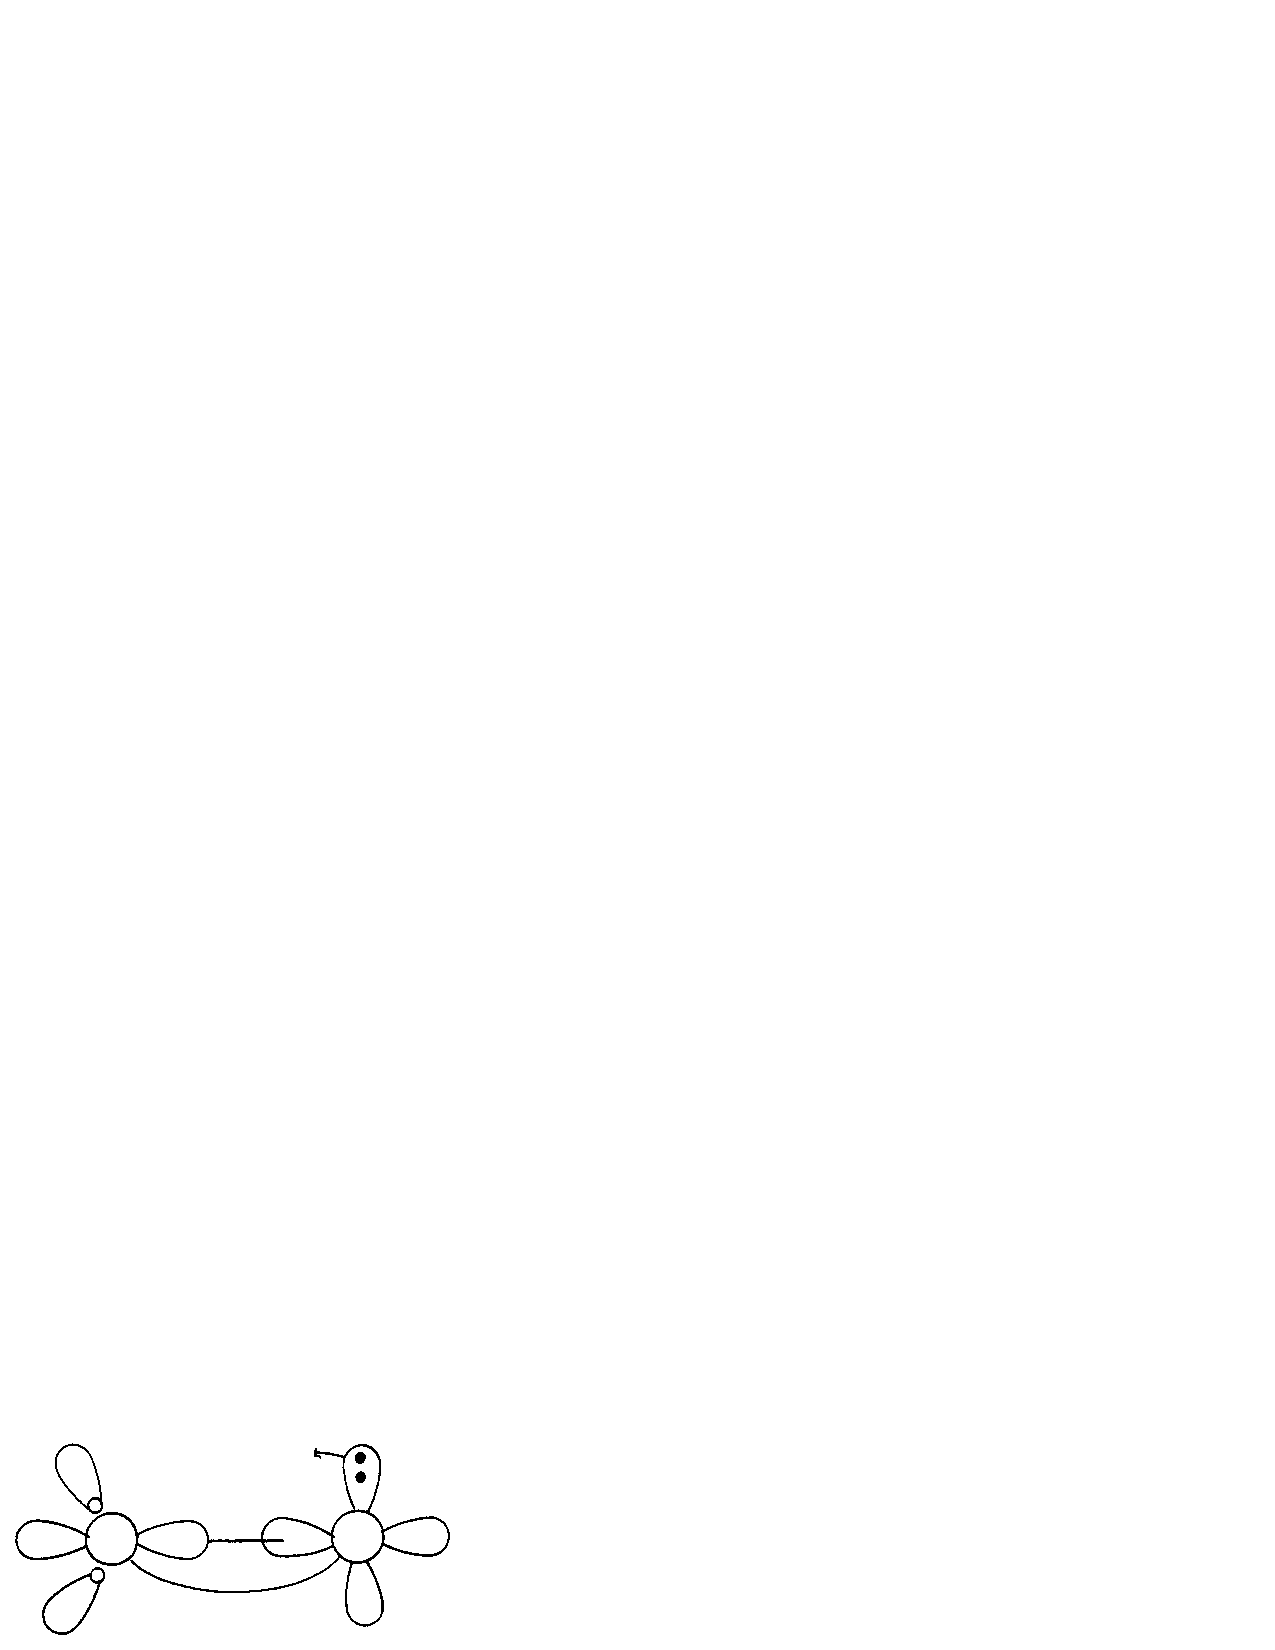
\includegraphics{fg13-2l}
\label{chap13-eqno8}
\end{equation}
and
\begin{equation}
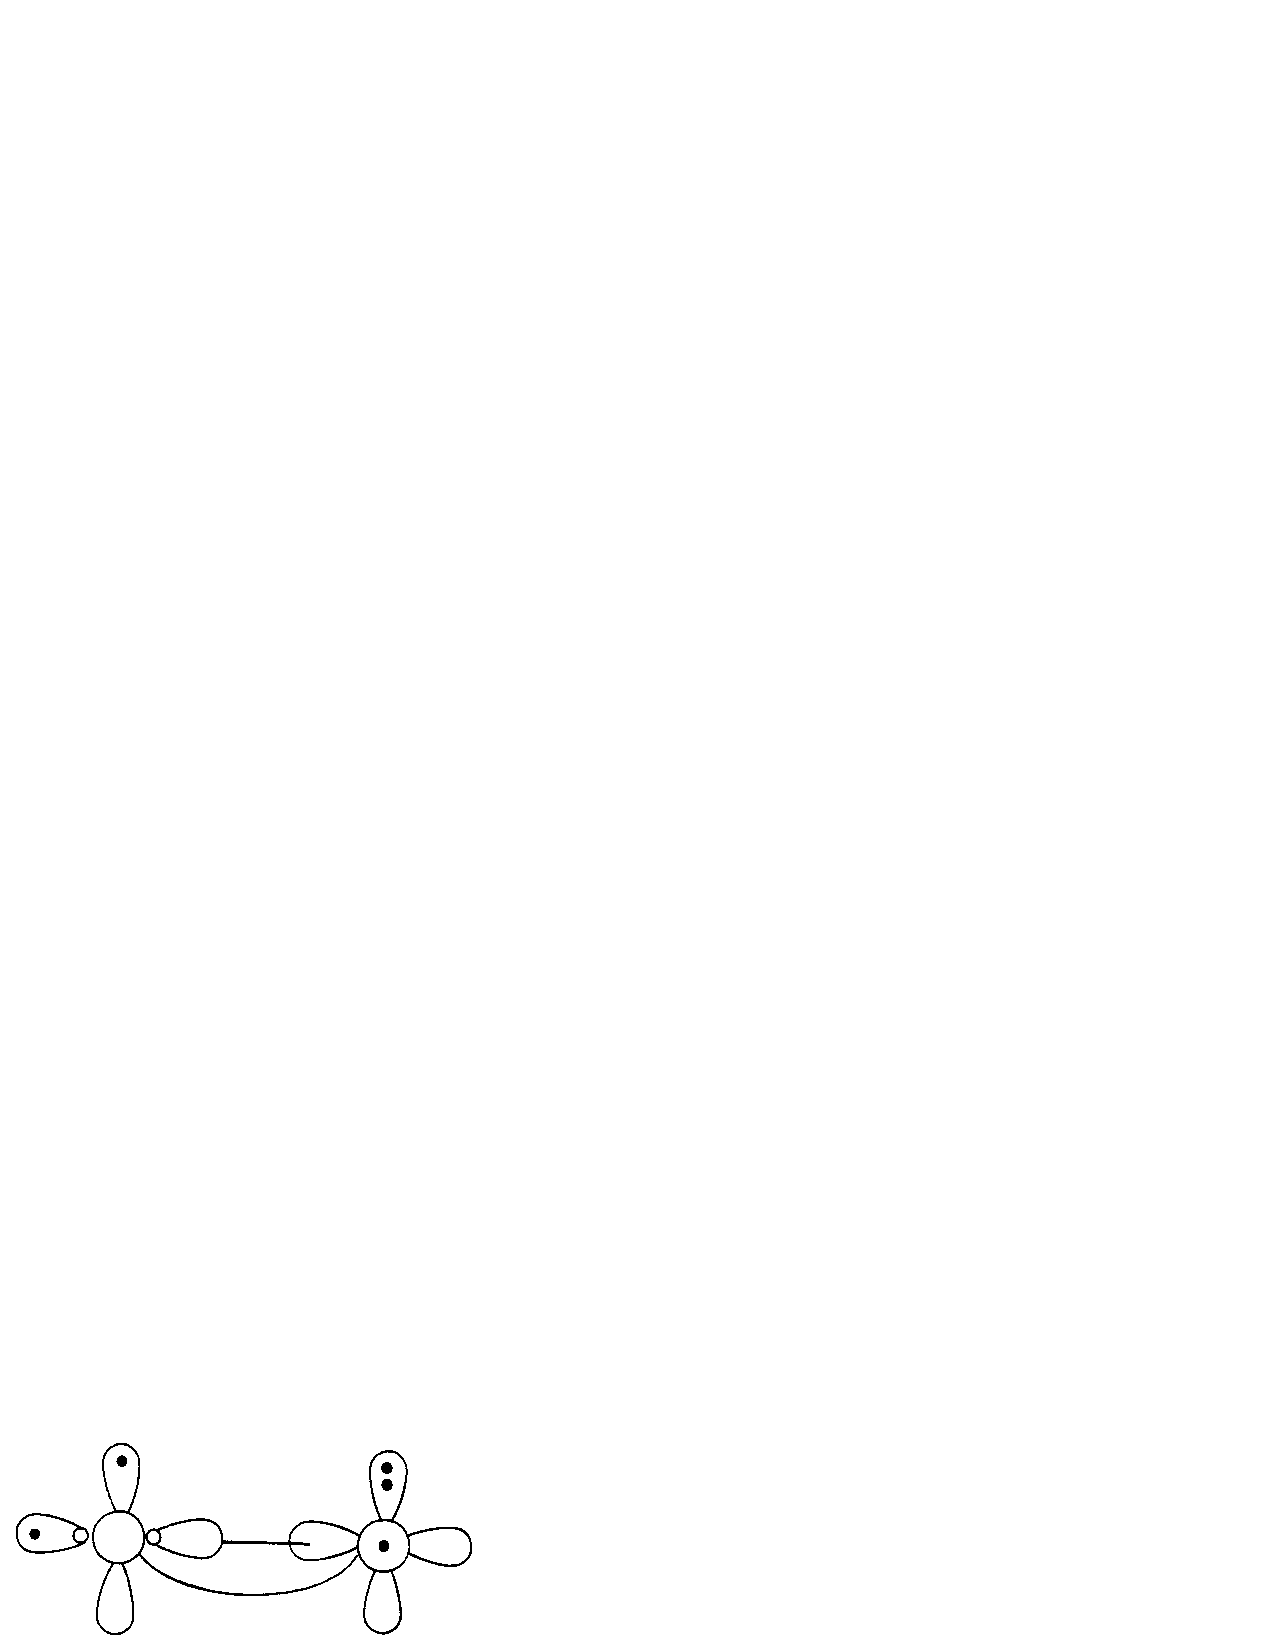
\includegraphics{fg13-2m}
\label{chap13-eqno9}
\end{equation}
as the low-lying states of CO.  The pi pairs of (\ref{chap13-eqno8})
become equivalent, as shown in Figure \ref{chap13-fig3}, and hence,
(\ref{chap13-eqno8}) describes the ${^1\Sigma}^+$ state.

\begin{figure}
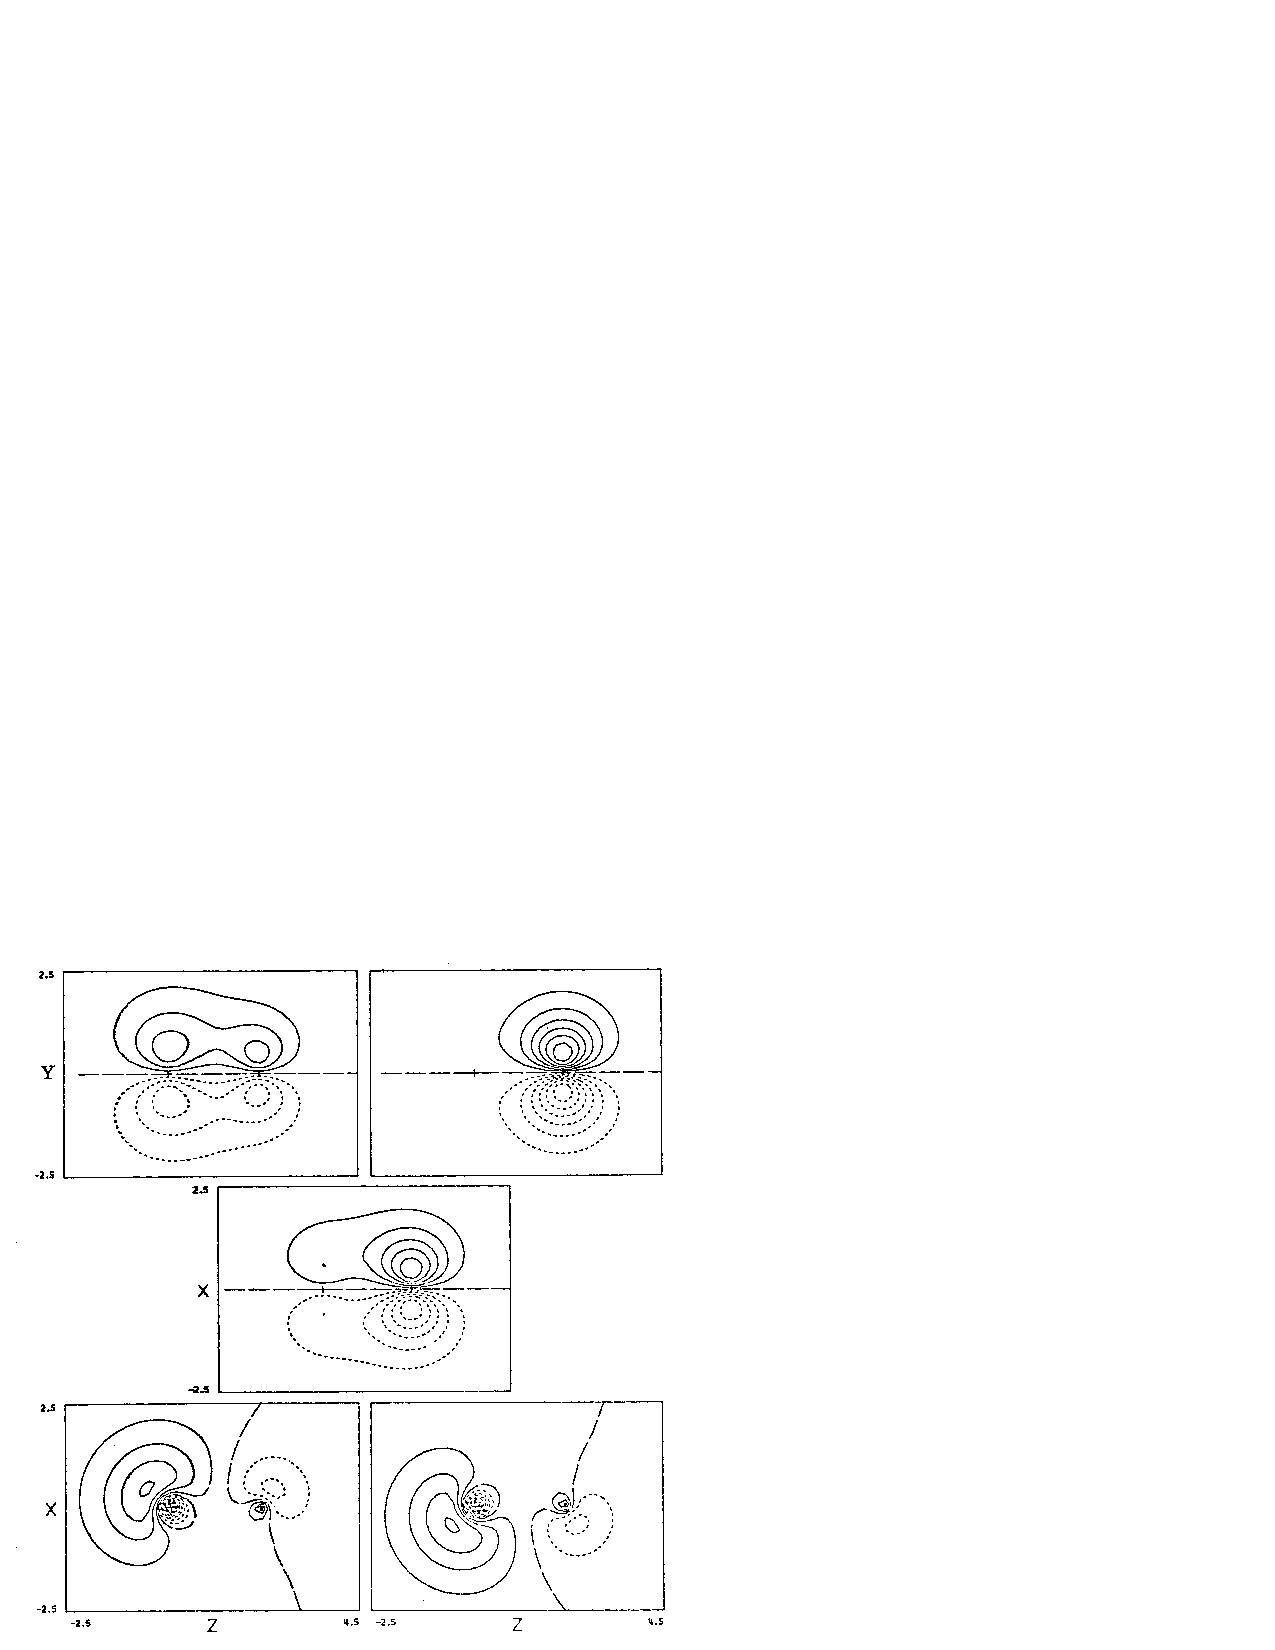
\includegraphics[scale=0.75]{fg13-3}
\caption{}
\label{chap13-fig3}
\end{figure}


Configuration (\ref{chap13-eqno9}) leads to ${^3\Pi}$ and ${^1\Pi}$
states of which ${^3\Pi}$ should be lower.  However, the ${^3\Pi}$
state involves an antibonding interaction between the $\pi_x$ pair on
the O and the $C \pi_x$ orbital.  As a result, the ${^3\Pi}$ state
should be much higher than the ${^1\Sigma}$ state.  In fact, it is 4
eV higher, as shown in Tables
\ref{chap13-tab4a}--\ref{chap13-tab4b}. The generalized valence bond
orbitals of the ${^3\Pi}$, and ${^1\Pi}$ states, are shown in Figures
\ref{chap13-fig3} and \ref{chap13-fig4}.

\begin{table}
\caption{First three states of CO.}
\label{chap13-tab4a}
\begin{tabular}{ccccccc}\\ \hline

& $T_o$ & $r_e$ & $\omega_e$ &\multicolumn{3}{c}{$D^0_o$}\cr
& (cm$^{-1}$) & (cm$^{-1}$) & (\AA) & (cm$^{-1}$) & (kcal) & (eV)\cr

X $^1\Sigma$ & 0 & 2169.8233 & 1.128322 & 89460 & 255.8 & 11.2\cr
a $^3\Pi$ & 48473.97 & 1743.55 & 1.2058 & 411121 & 117.5 & 5.1\cr
a$^{\prime}$ $^3\Sigma^+$ & 55353.91 & 1230.651 & 1.3519 & 34241 & 
97.9 & 4.2\cr

\hline
\end{tabular}
\end{table}

\begin{table}
\caption{First three states of CO$^+$.}
\label{chap13-tab4b}
\begin{tabular}{cccccc}\\ \hline

& $T_o$ & $r_e$ & $\omega_e$ &\multicolumn{2}{c}{$D^0_o$}\cr
& (cm$^{-1}$) & (cm$^{-1}$) & (\AA) & (cm$^{-1}$) & (kcal)\cr

X $^2\Sigma^+$ & 0 & 2214.24 & 1.1152 & 67309 & 192.4\cr
A $^2\Pi$ & 20407.47 & 1562.06 & 1.2438 & 46902 & 134.1\cr
B $^2\Sigma^+$ & 45633.52 & 1734.18 & 1.1688 & 37538 & 107.3\cr

\hline
\end{tabular}
\end{table}

\begin{figure}
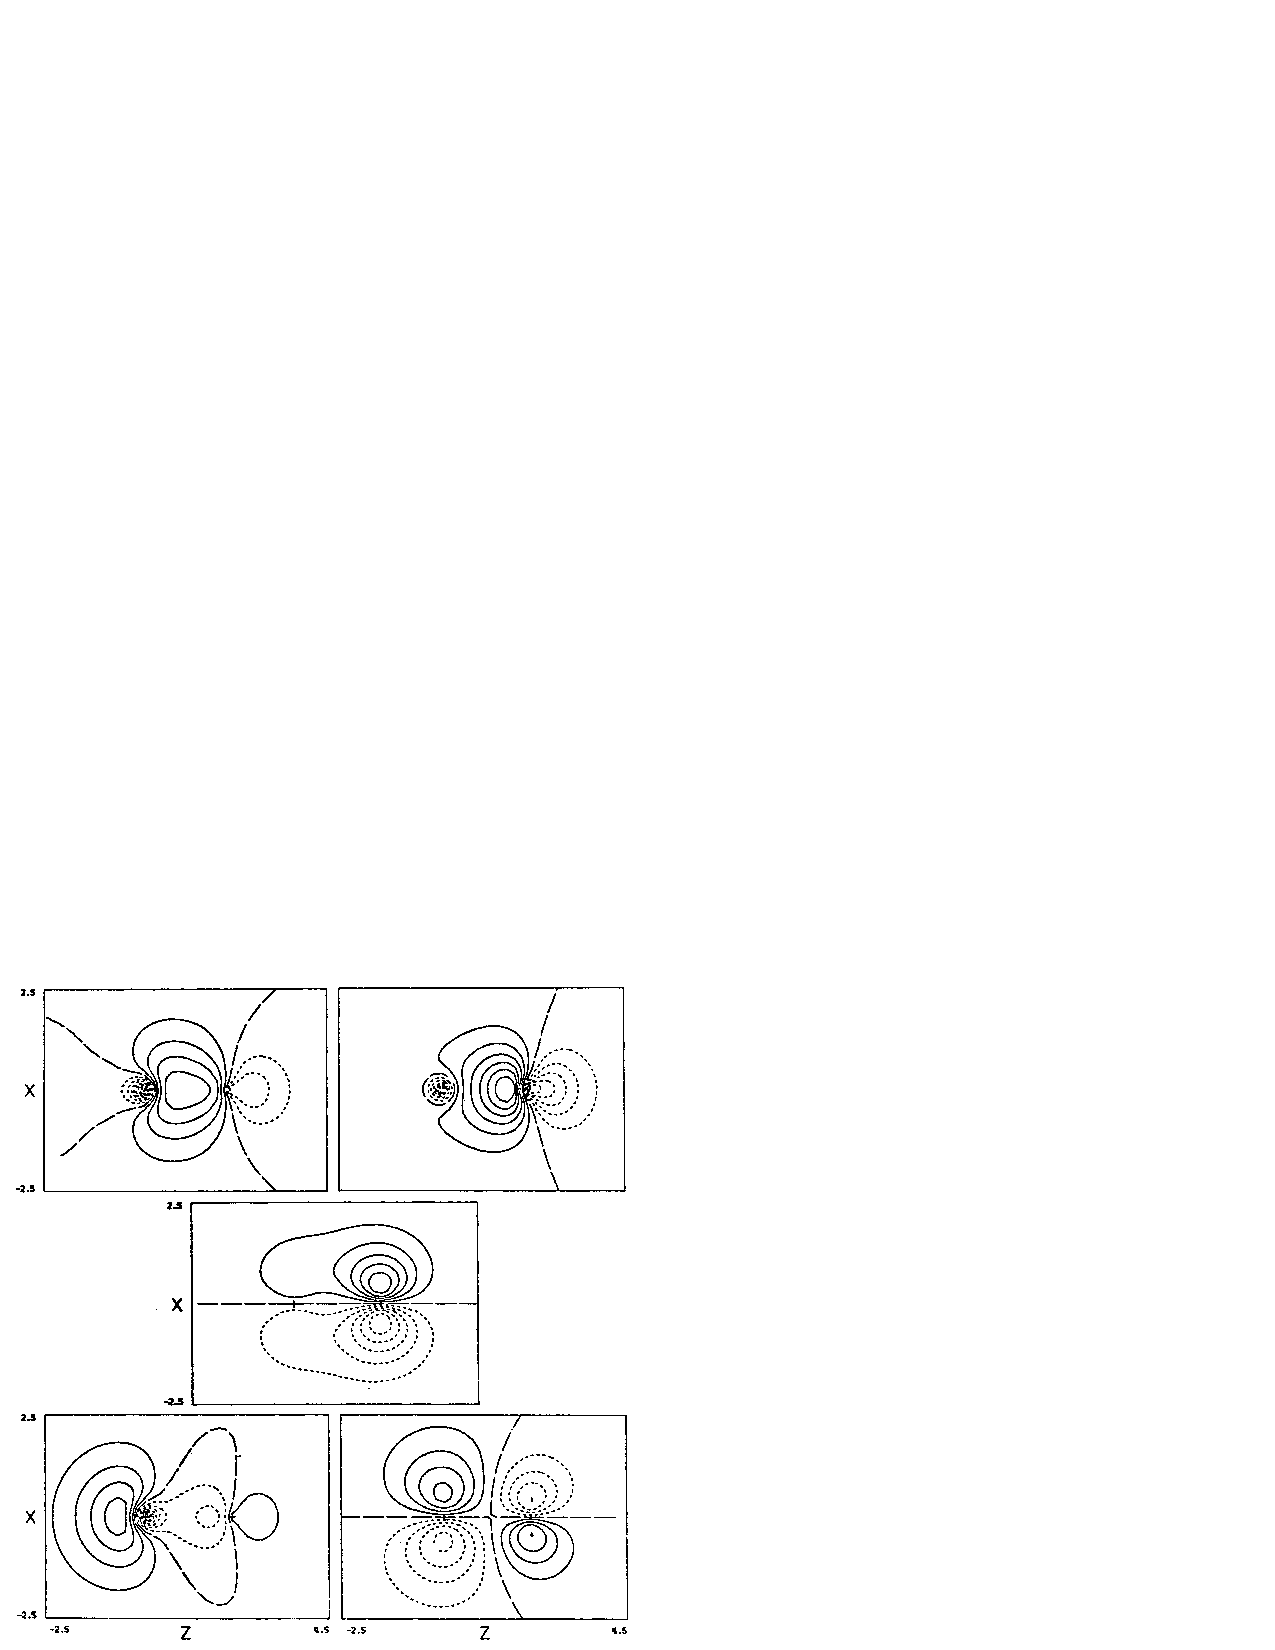
\includegraphics[scale=0.75]{fg13-4}
\caption{}
\label{chap13-fig4}
\end{figure}

There are three likely ways of ionizing an electron from the ground state 
of CO.  We can remove a C nonbonding orbital, leading to the 
${^2\Sigma}^+$ state
\begin{equation}
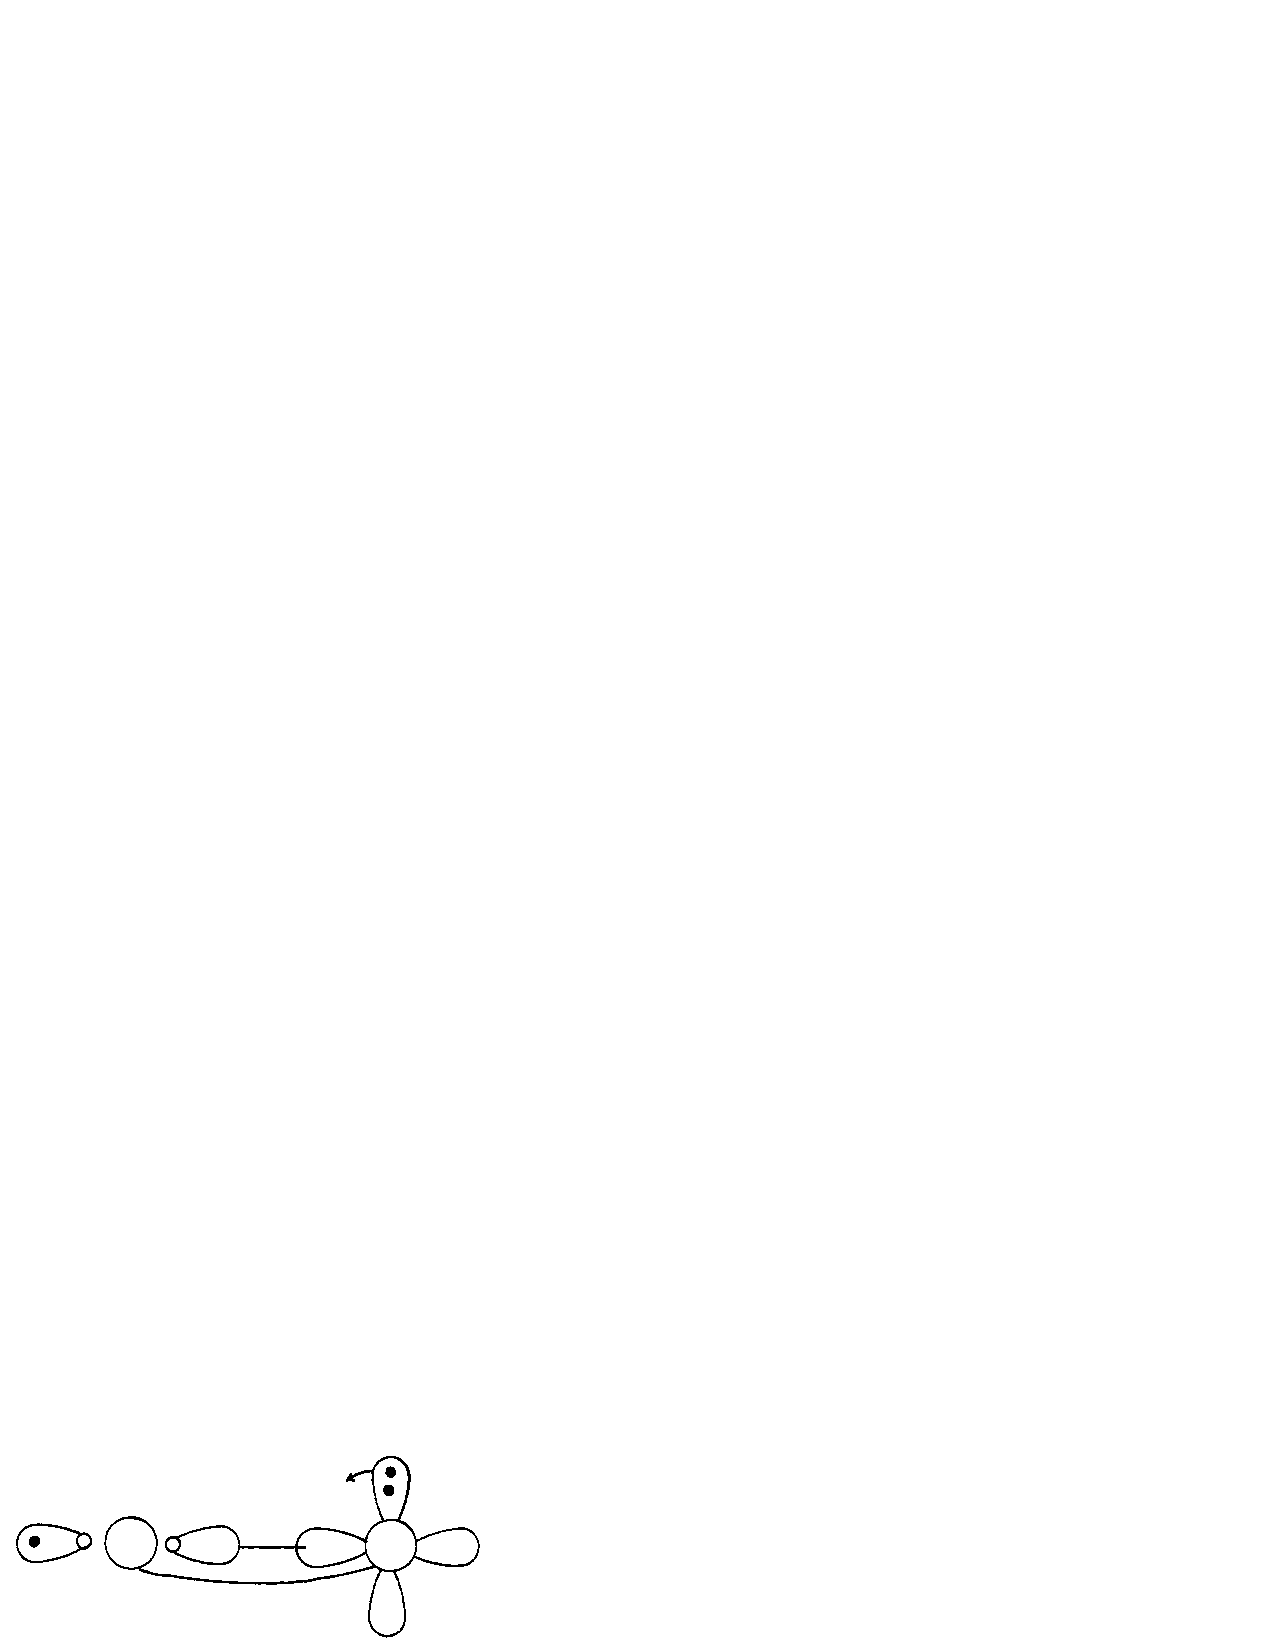
\includegraphics{fg13-4a}
\end{equation}
The two nonbonding orbitals of (\ref{chap13-eqno8}) are split away
from each other by their electron-electron repulsions, ionizing one
allows the other to rotate to the axis and get farther away from the
bonding pairs.  A second way is to remove a pi bonding orbital,
leading to a ${^2\Pi}$ state
\begin{equation}
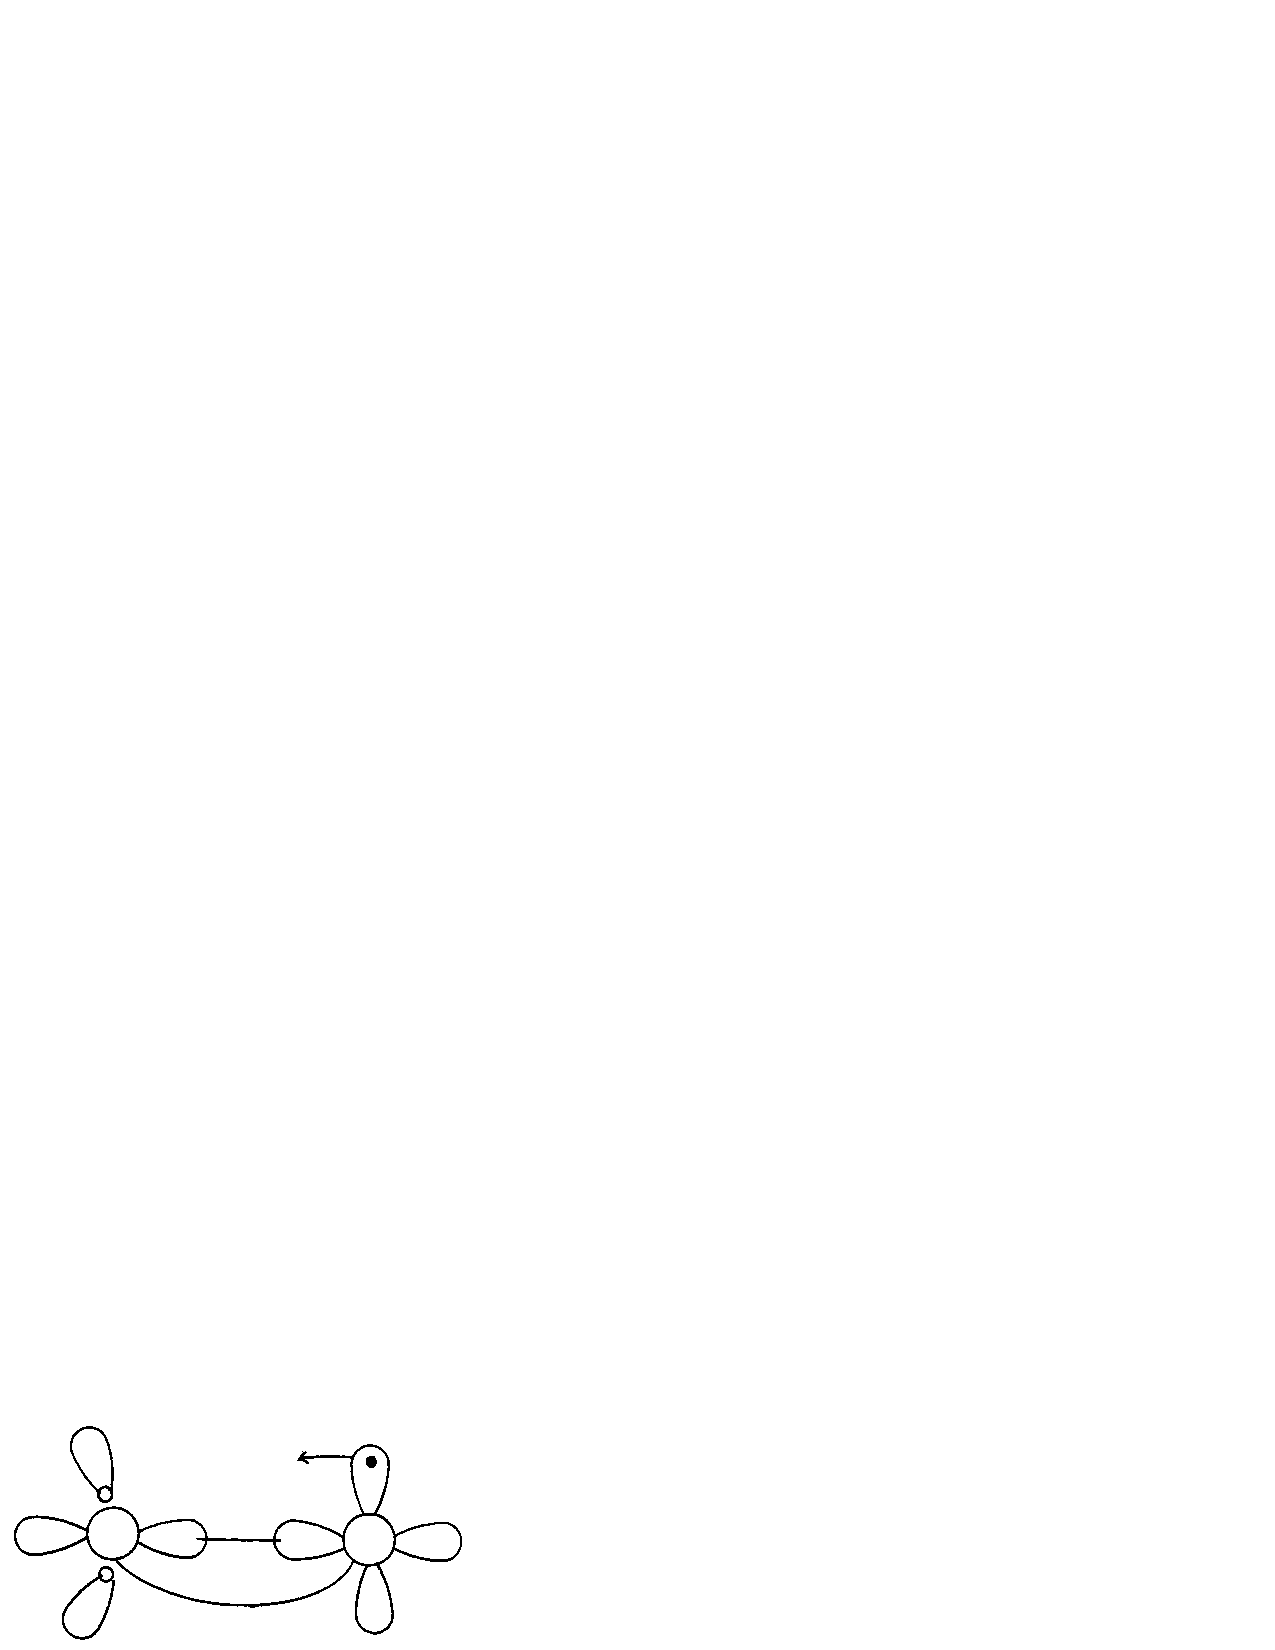
\includegraphics{fg13-4b}
\end{equation}
The third ionization is to remove an electron from the O2s orbital,
see the first row in Figure \ref{chap13-fig3},
\begin{equation}
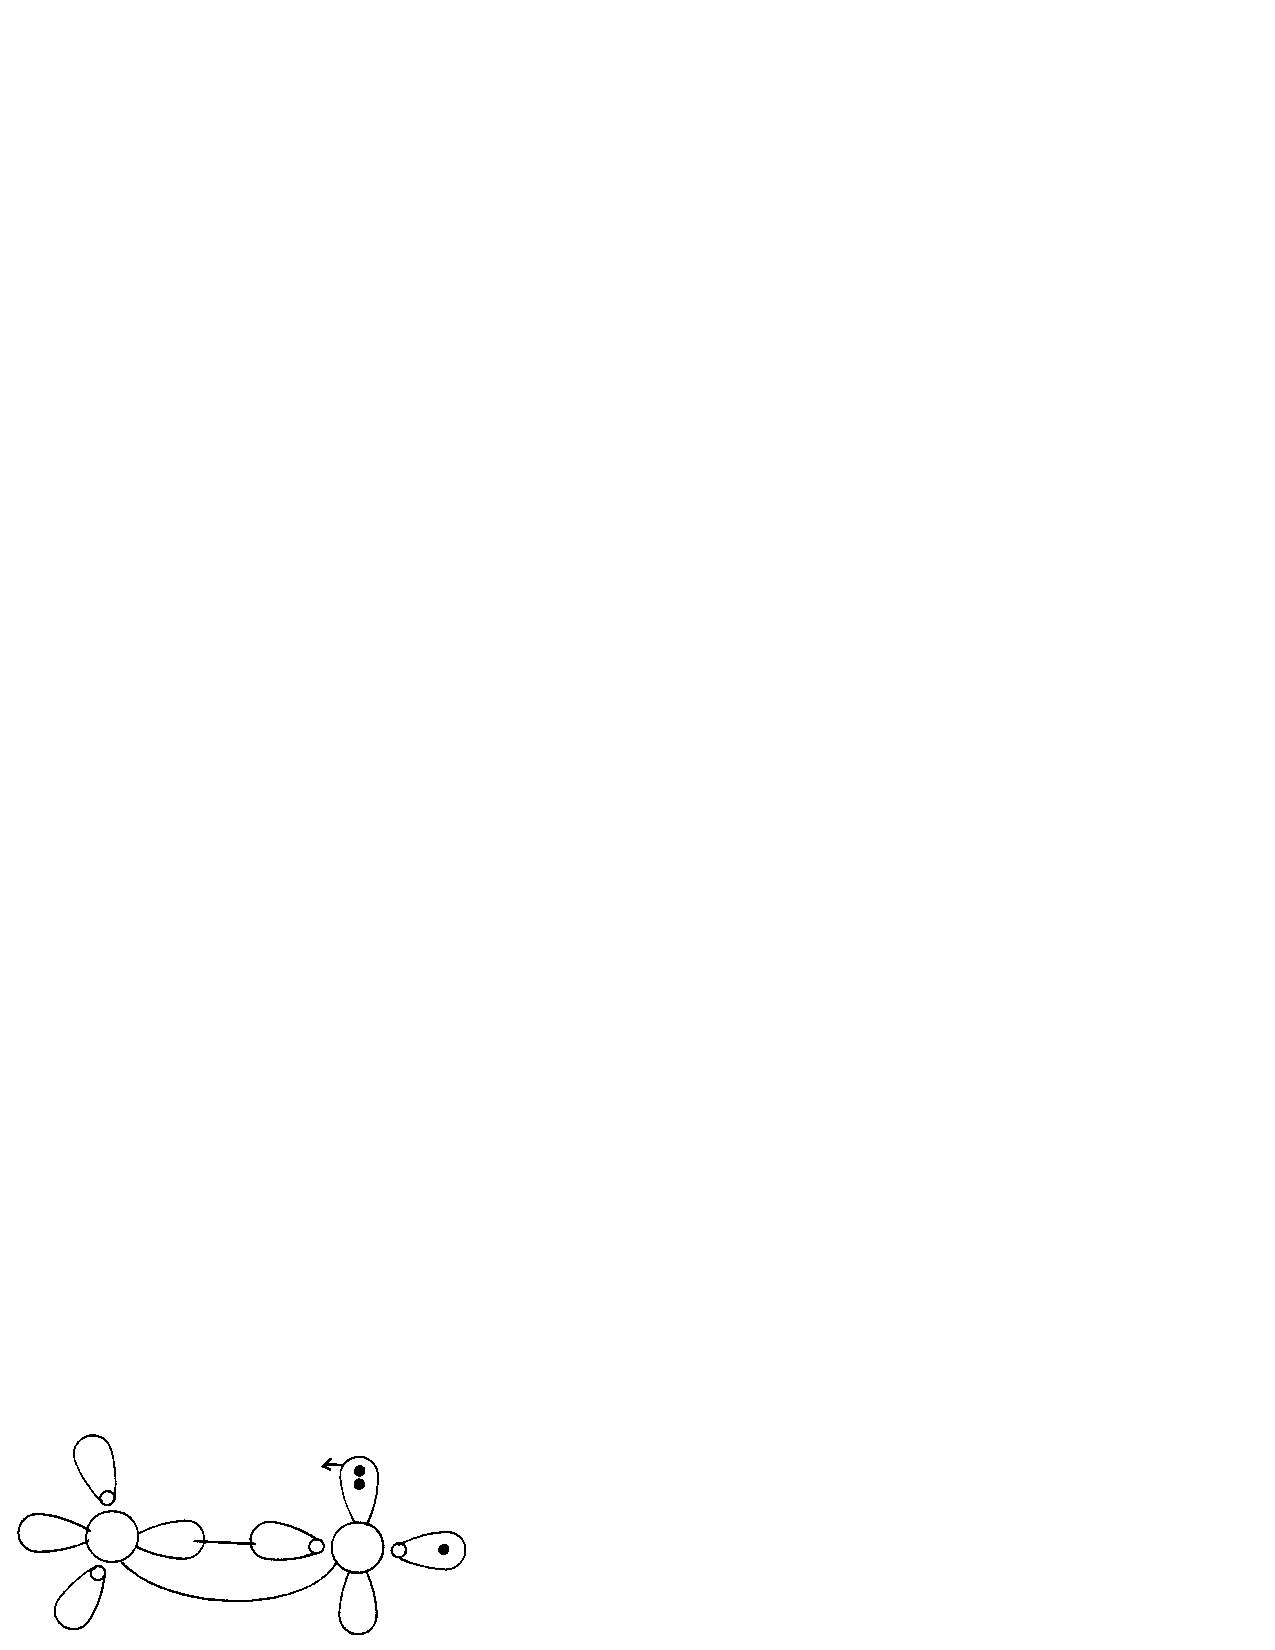
\includegraphics{fg13-4c}
\end{equation}
leading to another ${^2\Sigma}^+$ state. As shown in Tables
\ref{chap13-tab4a}--\ref{chap13-tab4b}, these are the lowest three
states of CO$^+$.

Note that removal of the C nonbonding orbital leads to a very slight 
decrease, .013 \AA, in $r_e$ and a slight increase, 45 cm$^{-1}$, in 
$\omega_e$, indicating the nonbonding character of
this orbital. The pi orbitals are involved in bonding and removing one 
leads to an increase, .115 \AA, in $r_e$ and a decrease, 608 cm$^{-1}$ , 
in $\omega_e$.

Removing the O nonbonding electron would be expected to also lead to small
changes in $r_e$ and $\omega_e$ except that removal of the O core electron 
should lead to large changes in the other sigma orbitals as they shift 
toward the O.  The result is an increase of 0.040 \AA\ in $r_e$ and a 
decreased of 435 cm$^{-1}$ in $\omega_e$.  One might view the loss of 
bonding here as due to partial removal of the bonding pair from the bond 
region.

Next, we will consider the dipole moments of the state of CO.  In the
ground state, we expect a large shift of sigma orbitals, from left to
right, O is much more electronegative than C.  The $\pi_y$ bond of
(\ref{chap13-eqno8}) would also be expected to be ionic toward the O
but the $\pi_x$ pair should be shifted toward the C. The generalized
valence bond orbitals average over these shifts. The net change, due
to the pi part of the system, is probably small.  However, the C
nonbonding lobe orbitals rotate behind the C, leading to a large shift
of electrons to the left. The net effect of the shift of electrons to
the right in ionic bonds and the shift to the left due to the C lobe
orbitals, should be a small dipole moment, in agreement with the
experimental results, $\mu = .11$ Debye, and sign C$^-$O$^+$.

In the ${^3\Pi}$ and ${^1\Pi}$ states, there is again a shift of
electrons to the O in the a bonding and O2s pairs, first two rows of
Figure \ref{chap13-fig5}. The bonding $\pi_y$ pair, third row, is
ionic toward the O but the O$\pi_y$ pair, fourth row, is back bonding
to the C and the C$\pi$ antibonding orbital, fifth row, is shifted to
the O. The net result in the pi electron would also seem to lead to
charge transfer to the 0. Thus, the ${^3\Pi}$ and ${^1\Pi}$ states of
CO should have large dipole moments with the sign C$^+$O$^-$.

\begin{figure}
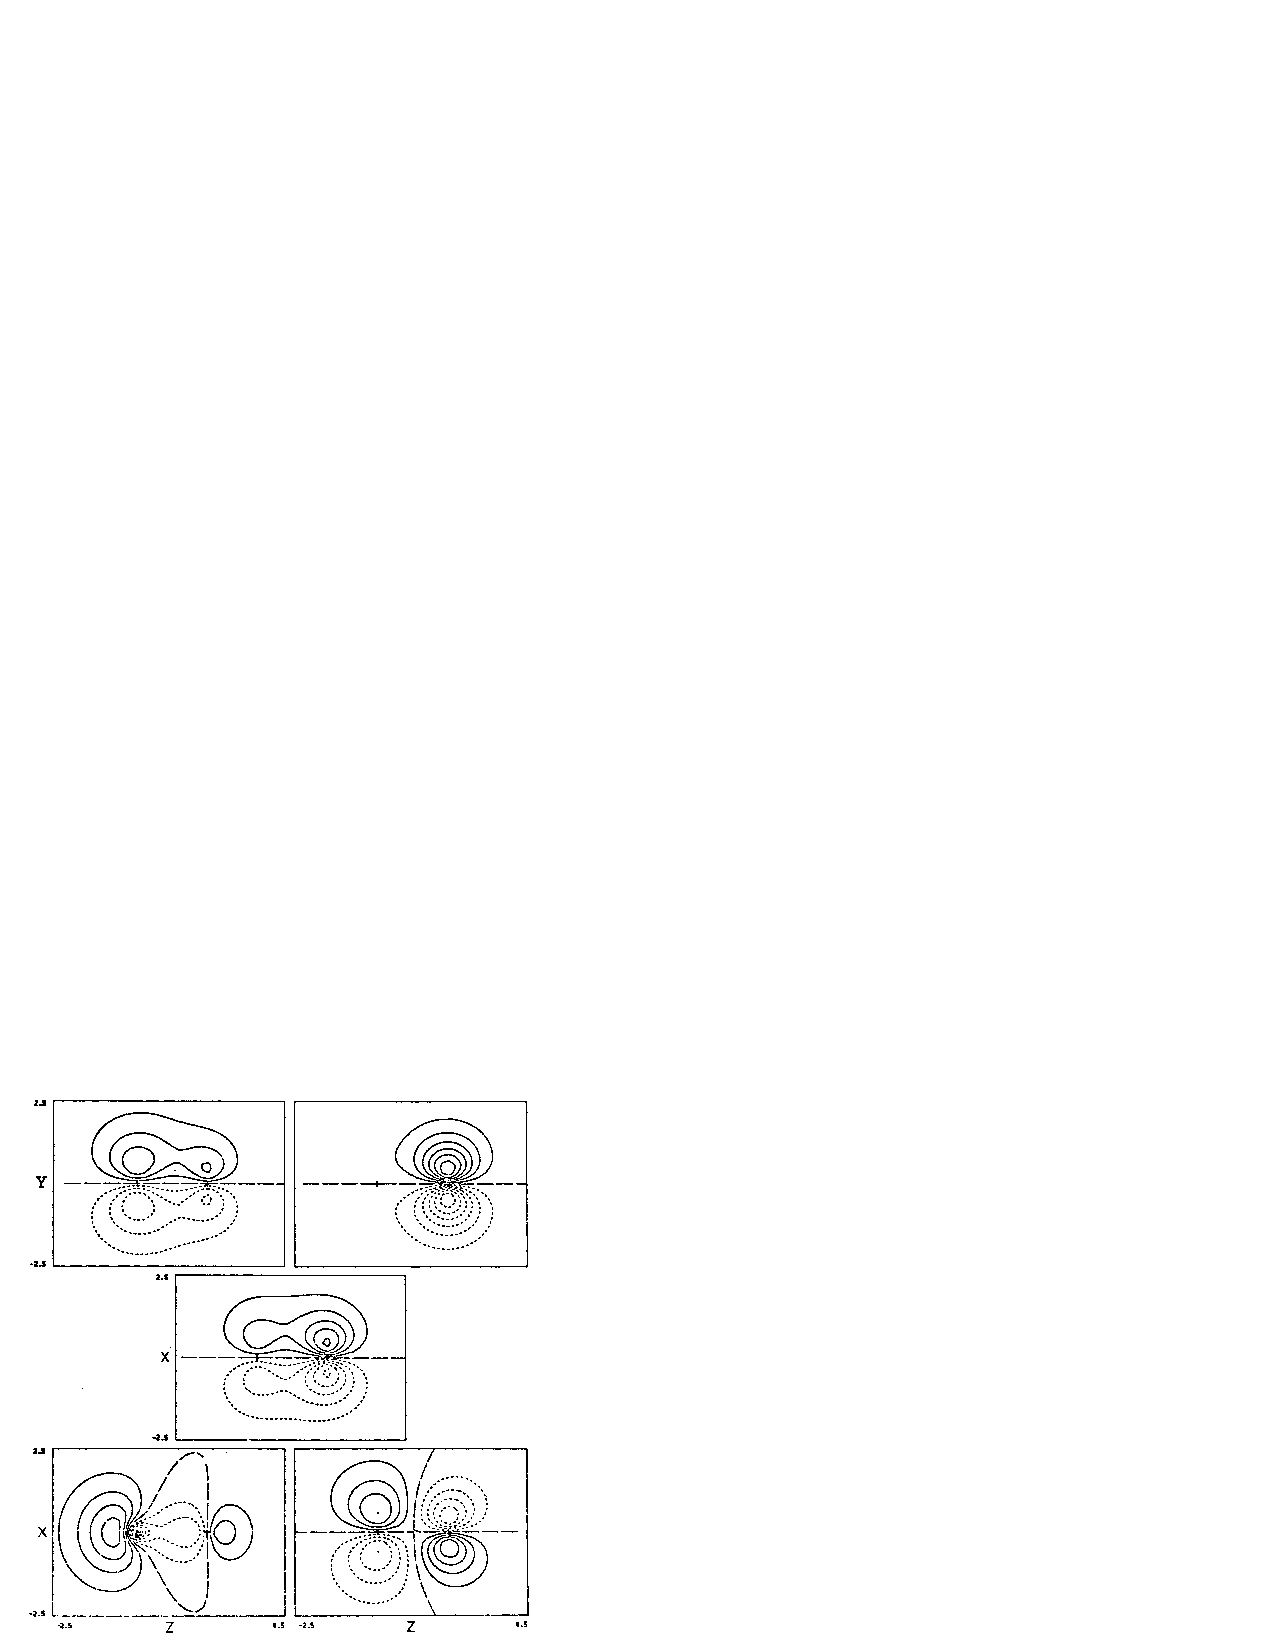
\includegraphics[scale=0.75]{fg13-5}
\caption{}
\label{chap13-fig5}
\end{figure}

Comparing the ${^3\Pi}$ and ${^1\Pi}$ states, they differ in the
exchange coupling between the unpaired orbitals, fourth row of Figure
\ref{chap13-fig4}, fifth row of Figure \ref{chap13-fig5}.  For the
${^3\Pi}$ state, this interaction favors having the sigma and pi
orbitals in the same region of space, leading to a sucking of the pi
orbital toward the C.  In the ${^1\Pi}$ state this interaction leads
to a pushing of the orbital away from the C.  The result is a larger
dipole moment C$^+$O$^-$ for the ${^1\Pi}$ state than for the
${^3\Pi}$ state.

\begin{table}
\caption{Generalized valence bond results for CO$^a$ 
where $R =$ 2.132 a$_0$.}
\label{chap13-tab5}
\begin{tabular}{cccccc}\\ \hline

& Energy &\multicolumn{3}{c}{Pair Information}&Dipole Moment\cr
& & Pair & $\Delta$E & $S_{ab}$ & (a.u.)\cr

$^1\Sigma^+$ & $-$112.0720 & b & .0086\cr
& & $\ell_c$ & .0093\cr
& & $\pi_y$ & .0308\cr
$^1\Sigma^+$ & $-$112.0857 & b & .0088 & .891 & $-$.2314\cr
& & $\pi_x$ & .0256 & .736\cr
& & $\pi_y$ & .0256 & .736\cr
$^3\Pi$ & $-$111.862 & b & .0062 & .9139\cr
& & $\pi_y$ & .0382 & .6655\cr
$^1\Pi$ & $-$111.7398 & b & .0054 & .9197 & .2965\cr
& & $\pi_y$ & .0304 & .7078\cr
\hline
\end{tabular}\\
$^a$MBS, SO, VB coupling.
\end{table}

The results of generalized valence bond calculation on CO, are
reported in Table \ref{chap13-tab5}.  In (\ref{chap13-eqno8}), the
O$\pi_x$ orbital is shown paired, however, this orbital becomes
bonding and should be allowed to split.  However, with both the lobe
pair and $\pi_x$ pair split the orbitals in these pairs become
overlapping.  The calculations reported here imposed strong
orthogonality and hence, cannot simultaneously allow both.  Thus, we
show in Table \ref{chap13-tab5} two separate calculations, the first
with the O$\pi_x$ orbital occupied and the second with the $\pi_x$
pair split but the C nonbonding orbital forced to be a sigma pair. The
latter restriction leads to a C orbital shifted too far to the left,
and hence, too negative a charge distribution.  Thus, the first
${^1\Sigma}^+$ state leads to a better description of the molecular
properties even though its energy is not as good.

\section{Molecules Formed from CO}

\subsection{HCO and H$_2$CO}

Starting from the ground state of CO
\begin{equation}
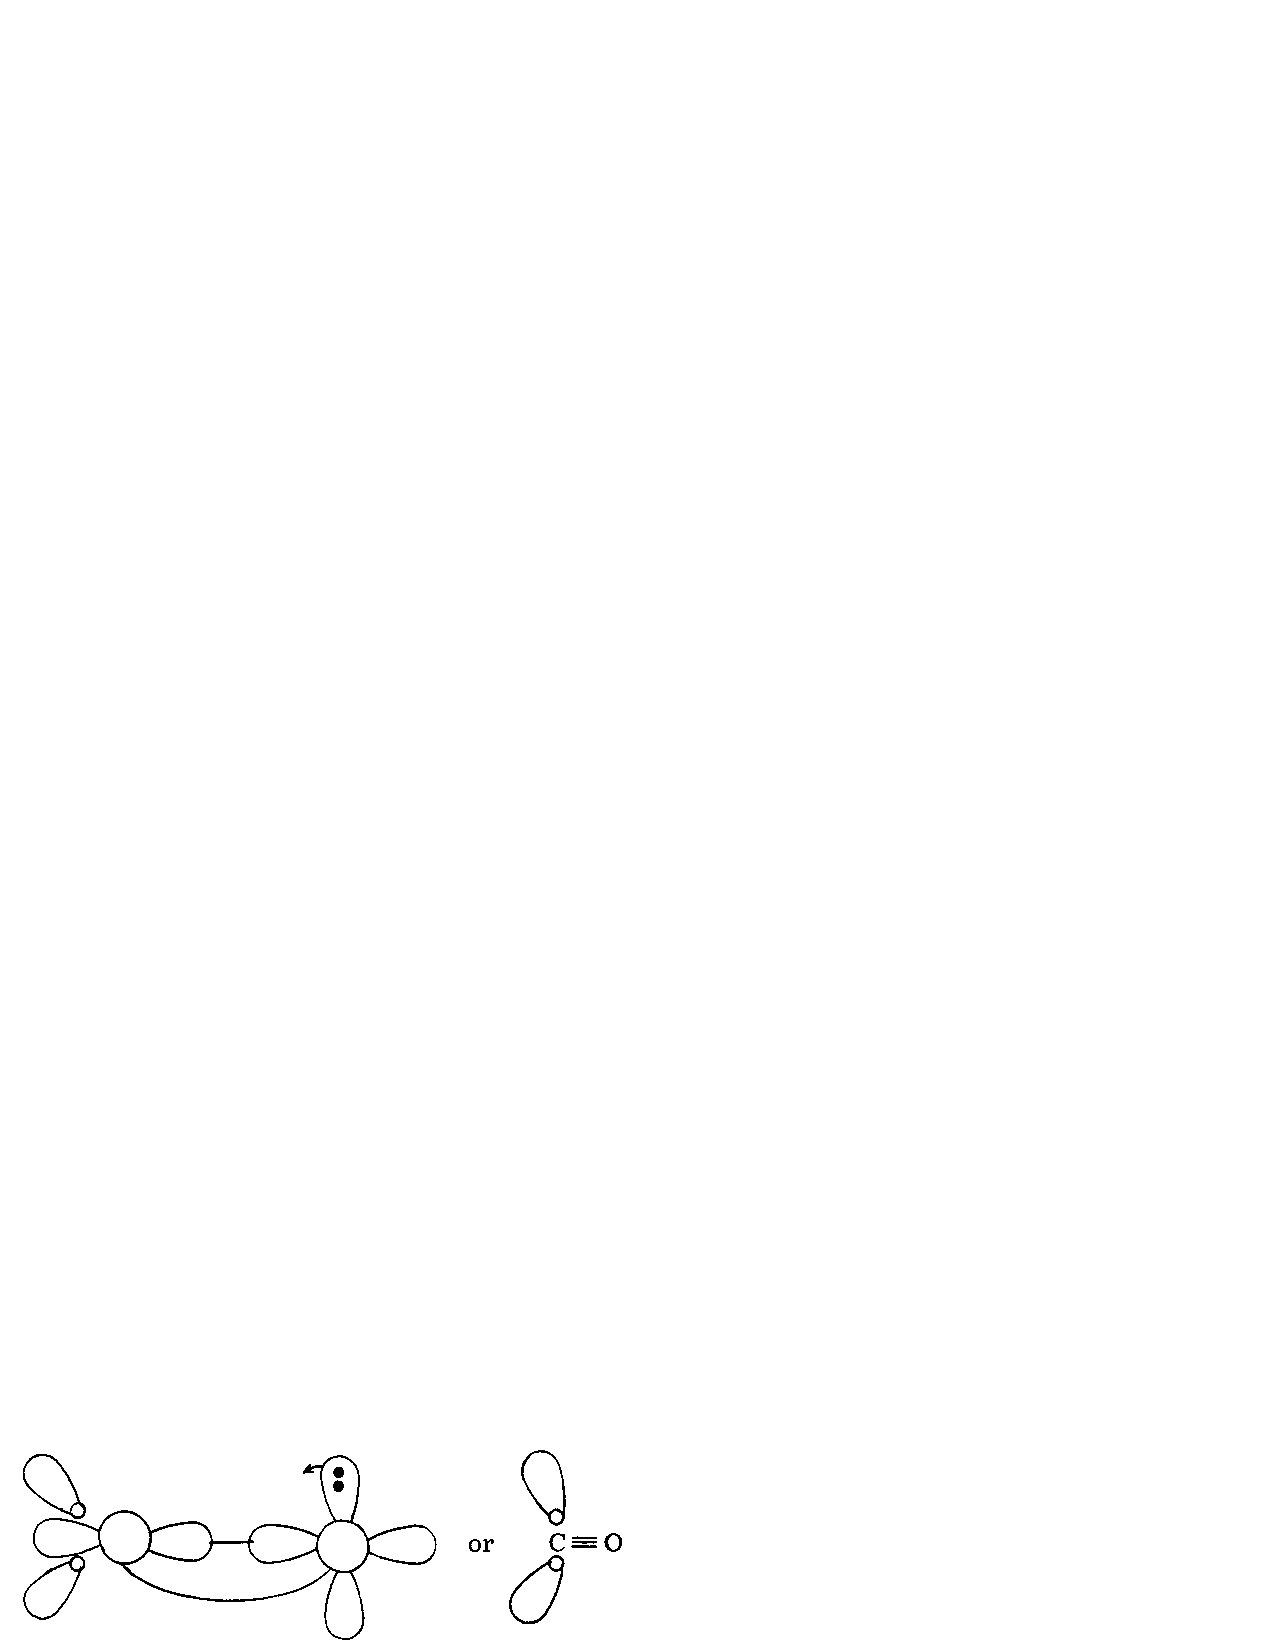
\includegraphics{fg13-5a}
\end{equation}
we can add an H to either lobe obtaining a bent HCO
\begin{equation}
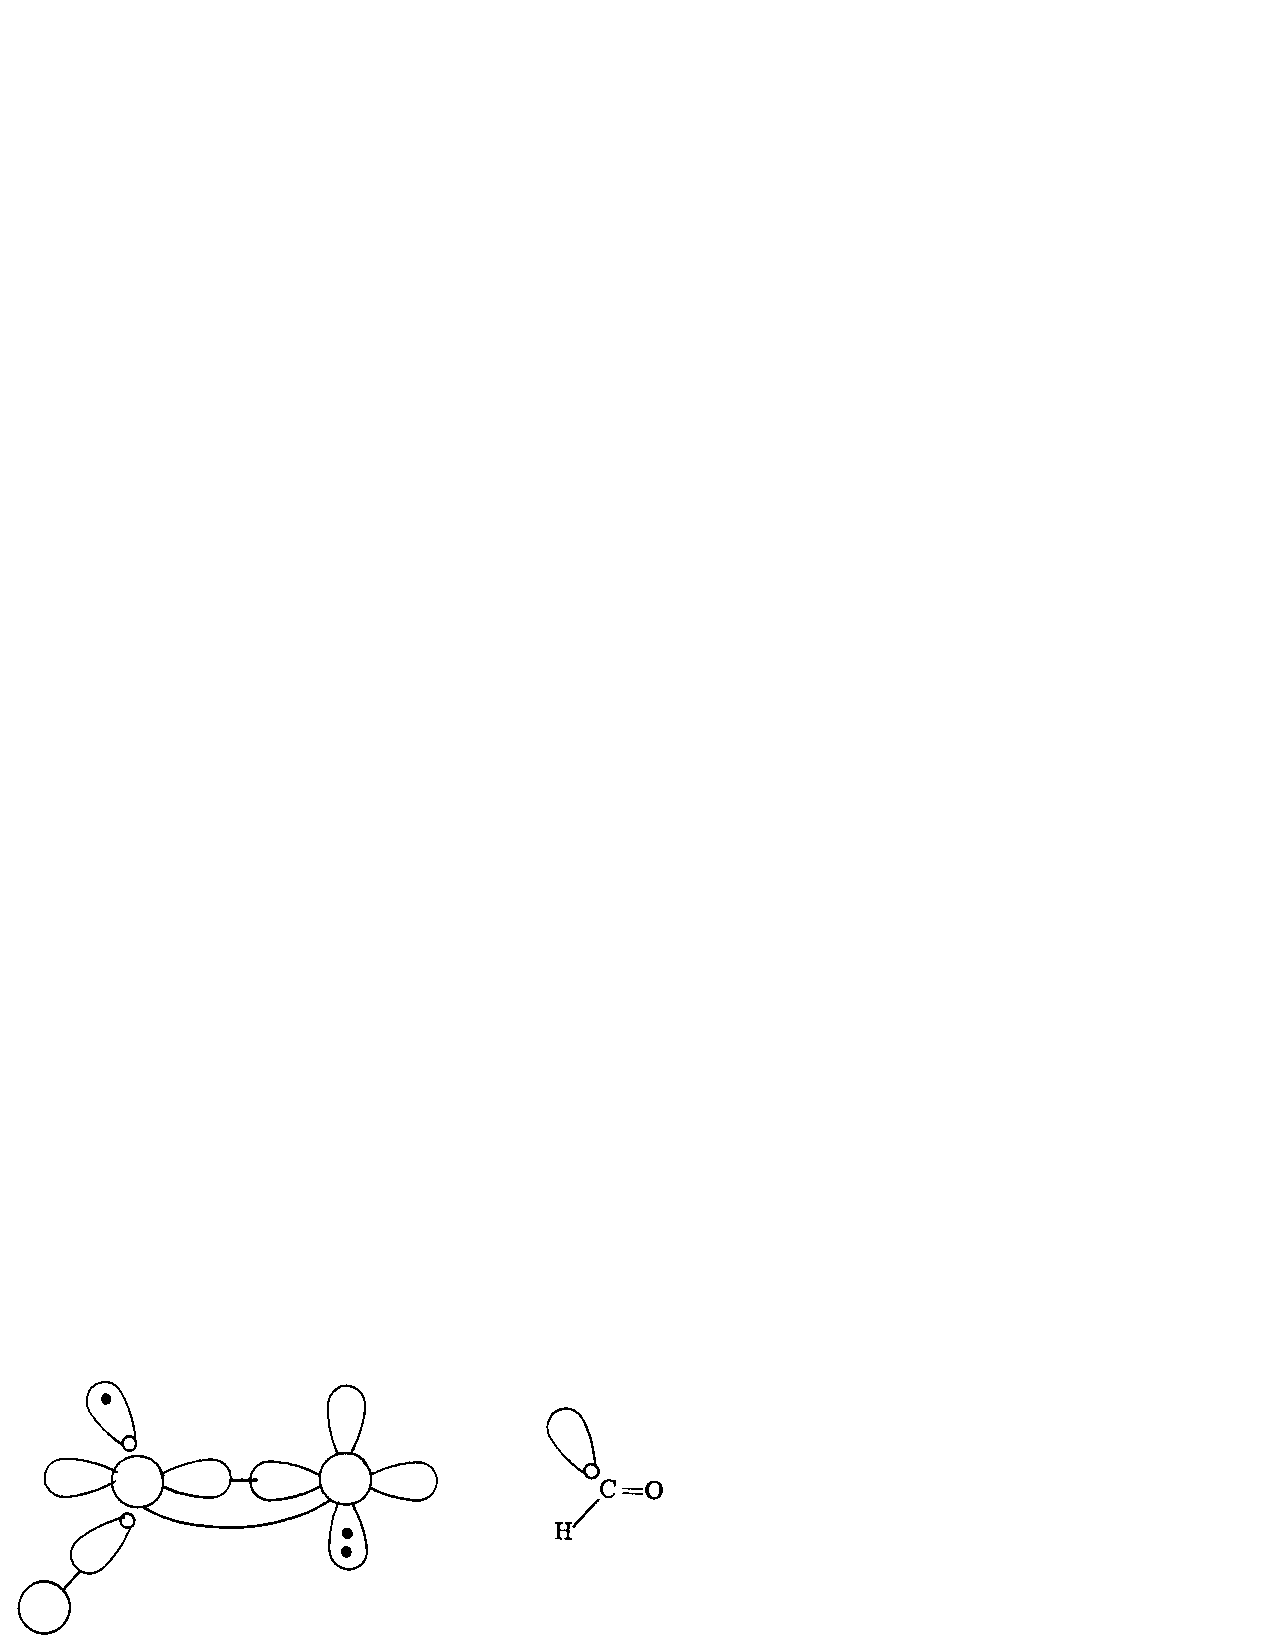
\includegraphics{fg13-5b}
\label{chap13-eqno10}
\end{equation}
The angle between the lobes of CO is about 85 degrees, so that for
large R the optimum HCO angle should be about 137 degrees.  Note that
there should be a small hump in the potential curve as the H is
brought up to the CO.  This small angle between the lobes occurs to
get these nonbonding orbitals out of the way of the CO sigma and
$\pi_x$ bonding pairs.  As we form a bond to the lobe orbital, we get
bad interactions between the new bond and the other lobe orbital,
leading to a decrease in the HCO bond angle.  In addition, having an
HC bonding pair in the xz plane makes it less favorable for the
O$\pi_x$ pair to delocalize into the C.  This would tend to weaken the
CO bond, larger $r_e$ and lower $\omega_e$, as observed, see Table
\ref{chap13-tab6}.

\begin{table}
\caption{The spectroscopic data on the states of HCO, 
third and fourth row, and the ground states of CO, first row, and H$_2$CO, 
last row.}
\label{chap13-tab6}
\begin{tabular}{ccccccccc}\\ \hline

& JP & $T_0$ & $r_{HC}$ & $r_{CO}$ & HCO & $\nu_{HC}$ & 
$\nu_{bond}$ & $\nu_{CO}$\cr
& (ov) & (cm$^{-1}$)\cr

X $^1\Sigma^+$ & 14.013 & -	& - & 1.128 & - & - & - & 2169.8\cr
X $^2A^{\prime}$ & 9.88 & .0 & (1.08) & 1.19$^8$ & 119.5$^{\circ}$ & 
(2700) & 1083.0 & 1820.2\cr
A $^2A^{\prime\prime}$ $^a$ & & 9294.$^0$ & 1.04$^4$ & 1.187 & 
180$^{\circ}$ & 3316.2 & 802.3 & 1812.4\cr
X $^1A_1$ & 10.88 & - & 1.102 & 1.210 & 119.5 & 2766.4 & 1500.6 & 
1746.1\cr
& & & & & & 2843.4 & 1167.\cr
\hline
\end{tabular}\\
$^a$($\pi$)C$_{\infty \nu}$.
\end{table}

The nonbonding orbital of (\ref{chap13-eqno10}) has nodal planes
running through the HC and CO bonds, leading to a shape as indicated
in Figure \ref{chap13-fig6}.

\begin{figure}
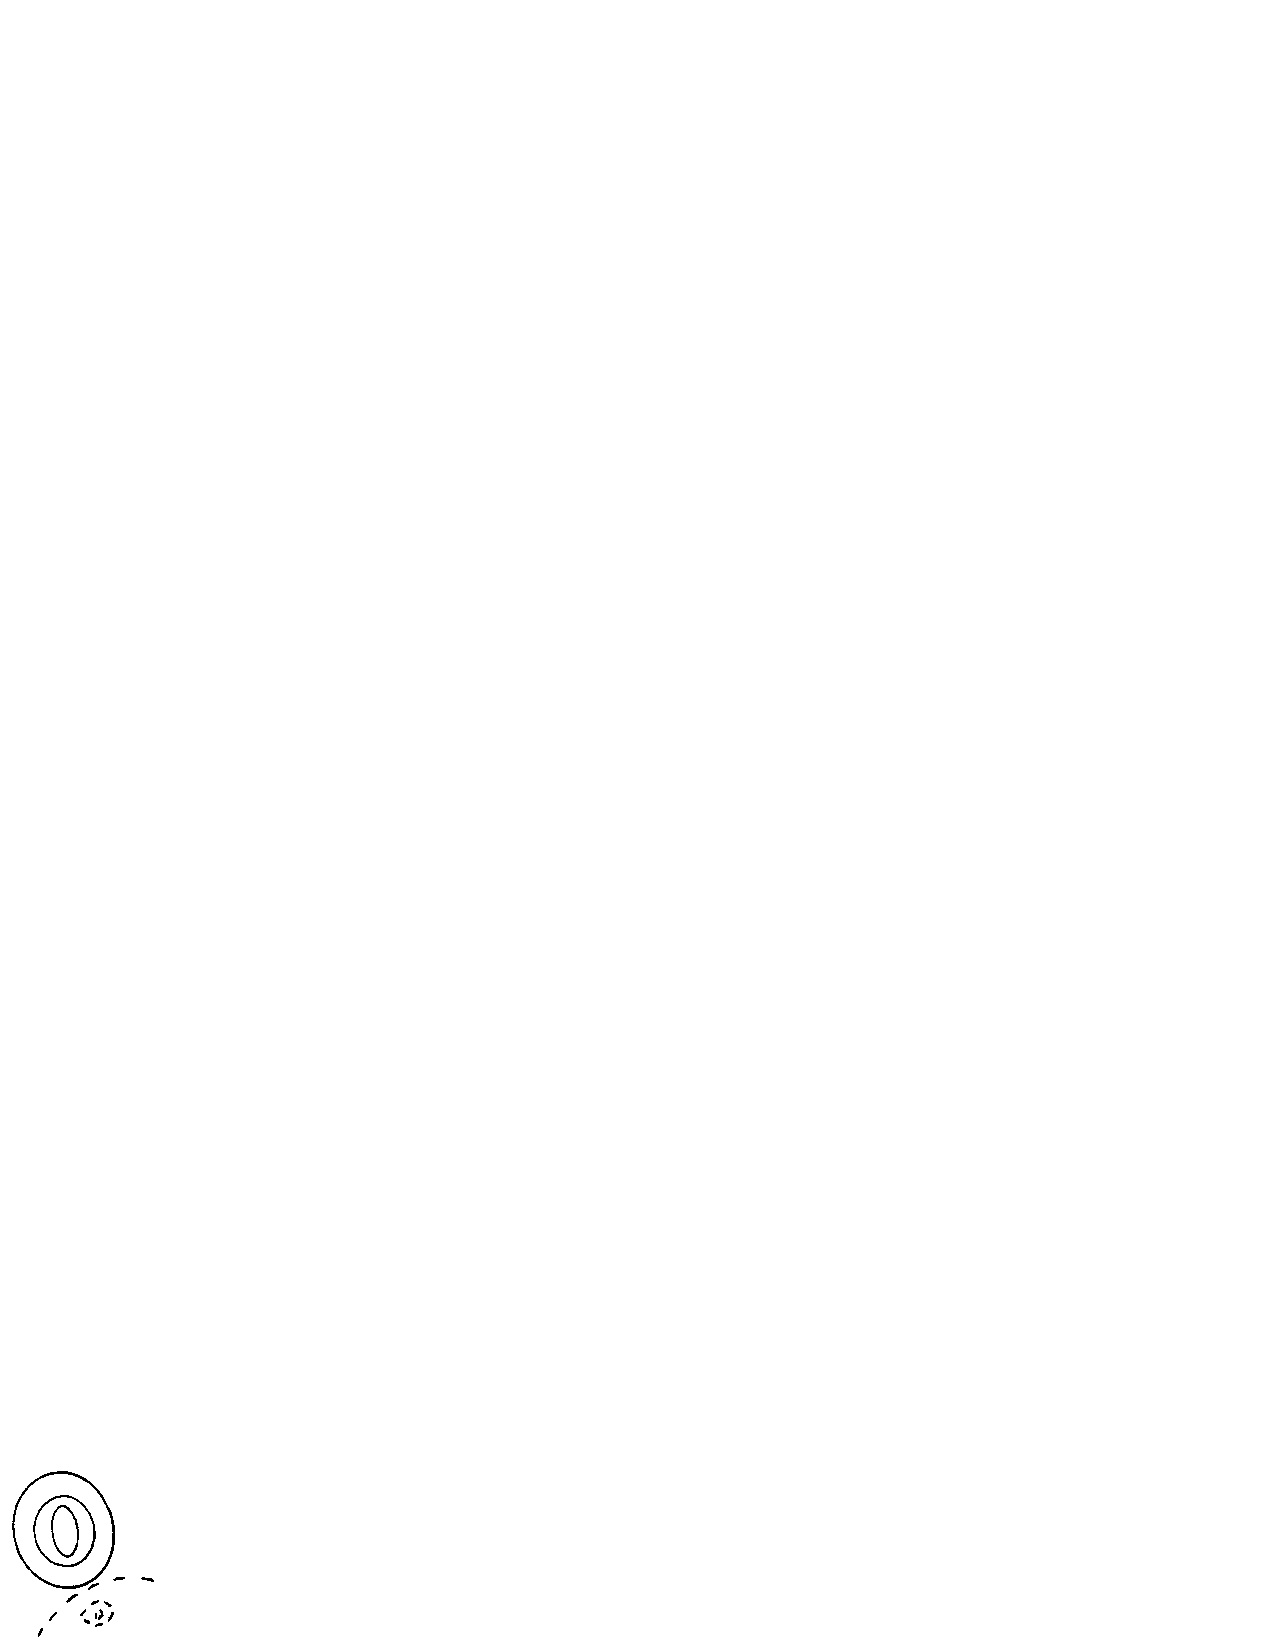
\includegraphics[scale=0.75]{fg13-6}
\caption{}
\label{chap13-fig6}
\end{figure}

As we straighten out the molecule, the nonbonding orbital becomes a pi 
orbital of the linear molecular
\begin{equation}
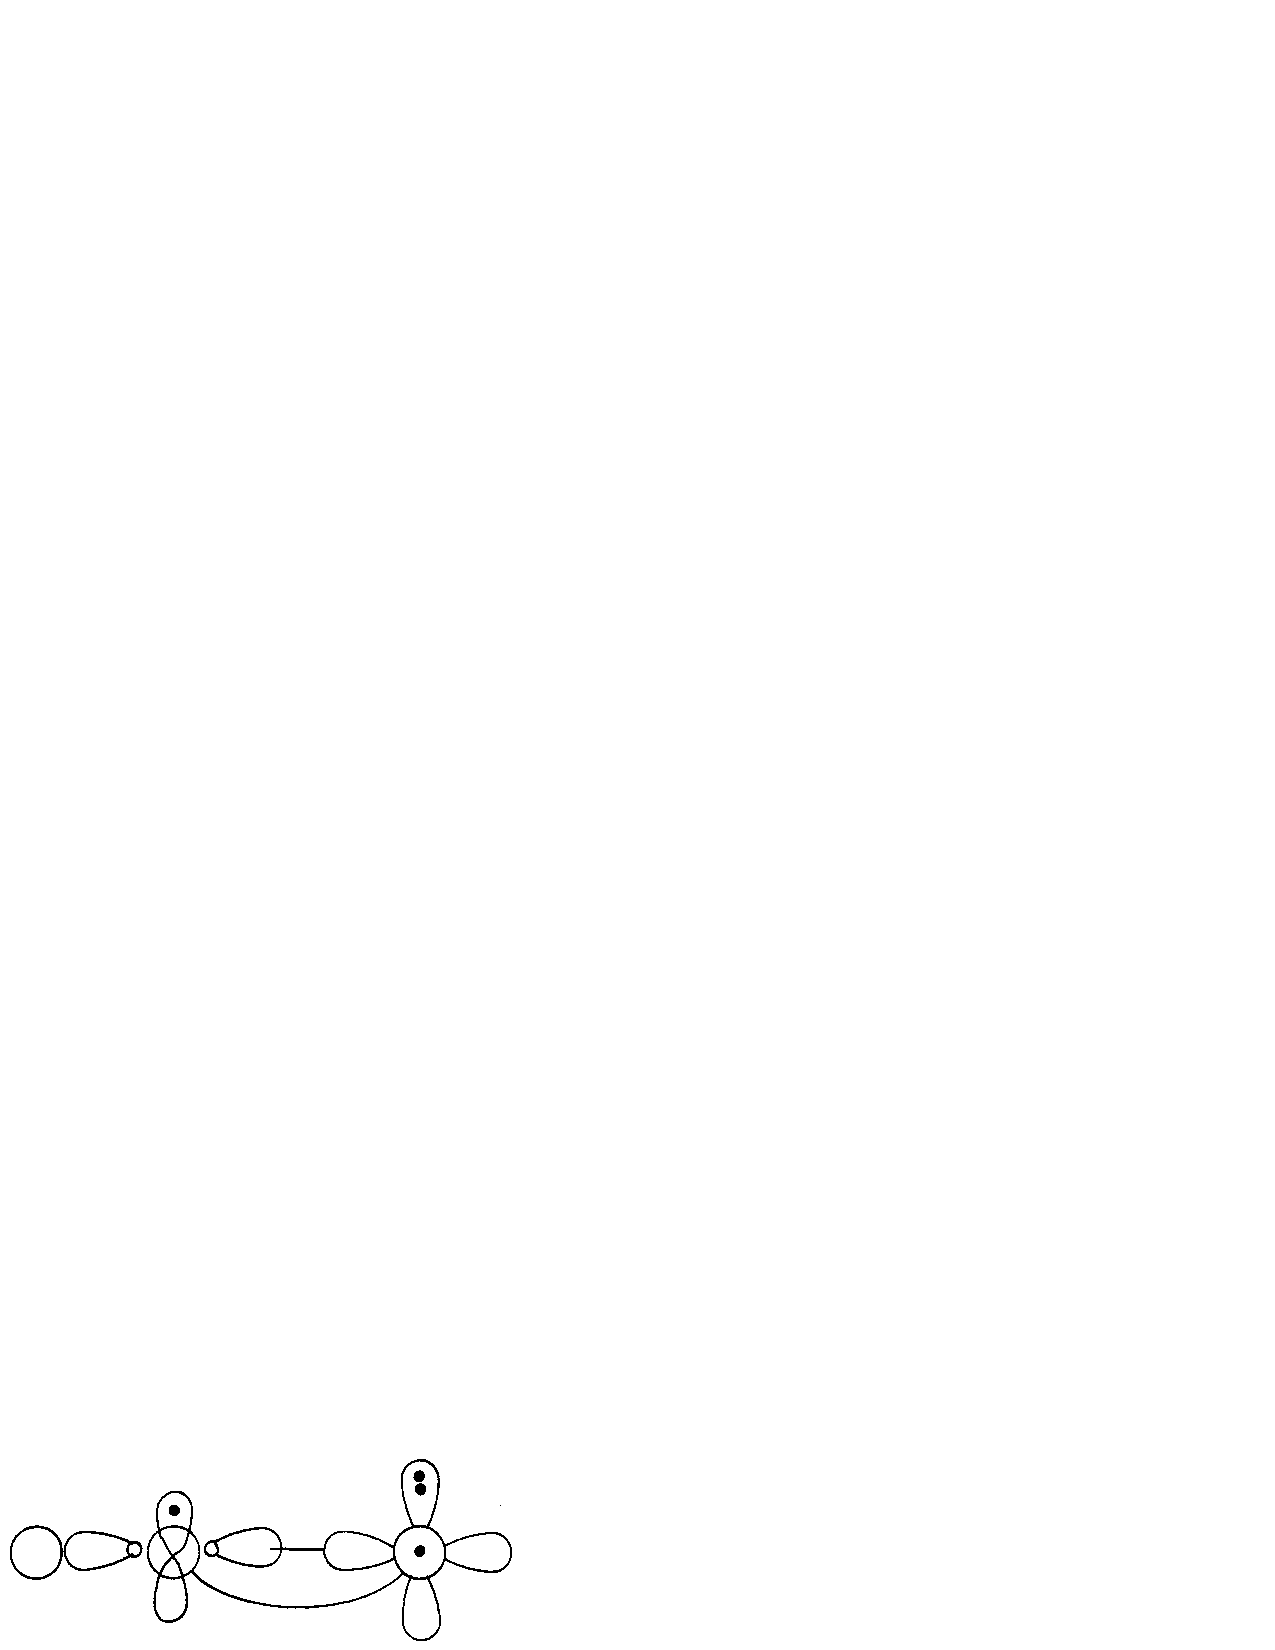
\includegraphics{fg13-6a}
\end{equation}
This is just one component of the ${^2\Pi}$ state of linear HCO.  The other 
has ${^2A}^{\prime \prime}$ symmetry upon bending
\begin{equation}
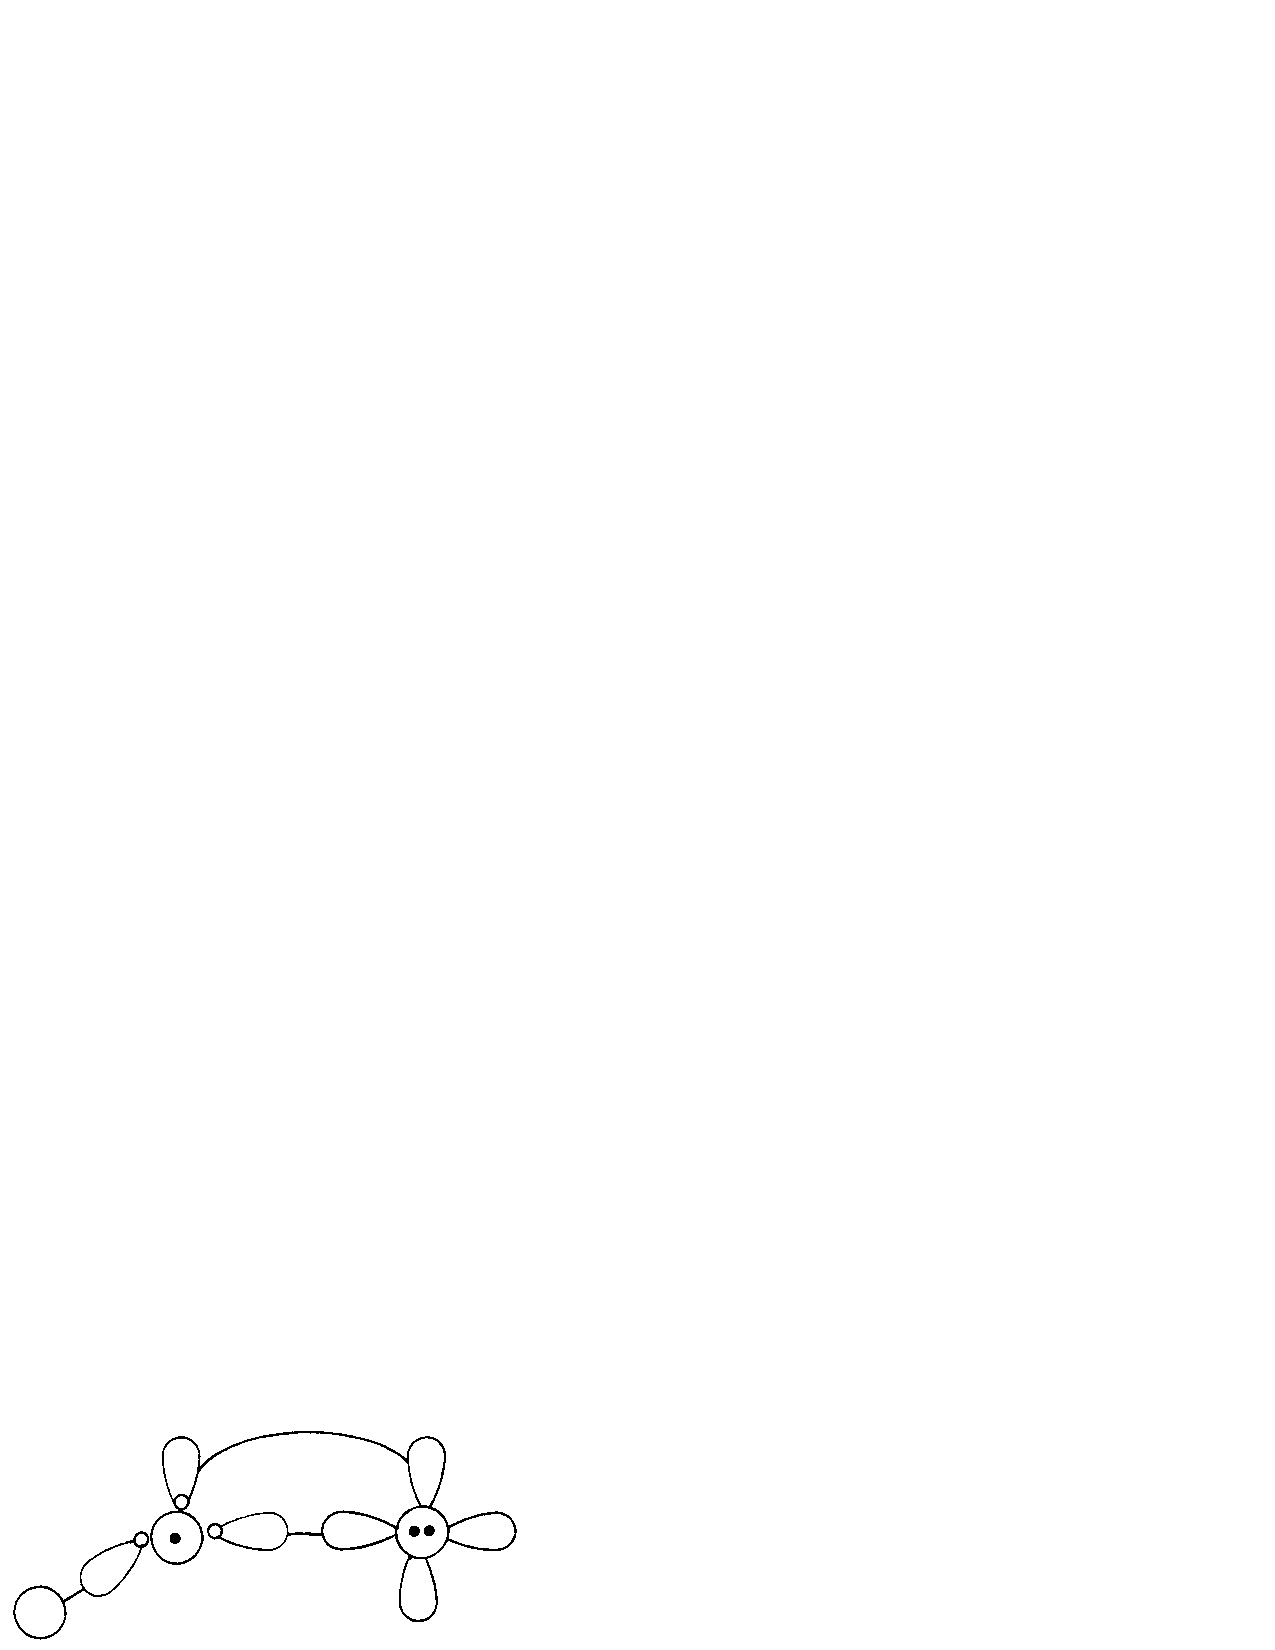
\includegraphics{fg13-6b}
\end{equation}
and, as would be expected, has a minimum for the linear geometry.

Starting with the ground state of HCO, (\ref{chap13-eqno10}) we expect
H$_2$CO, formaldehyde, to be strongly bound with the geometry,
\begin{equation}
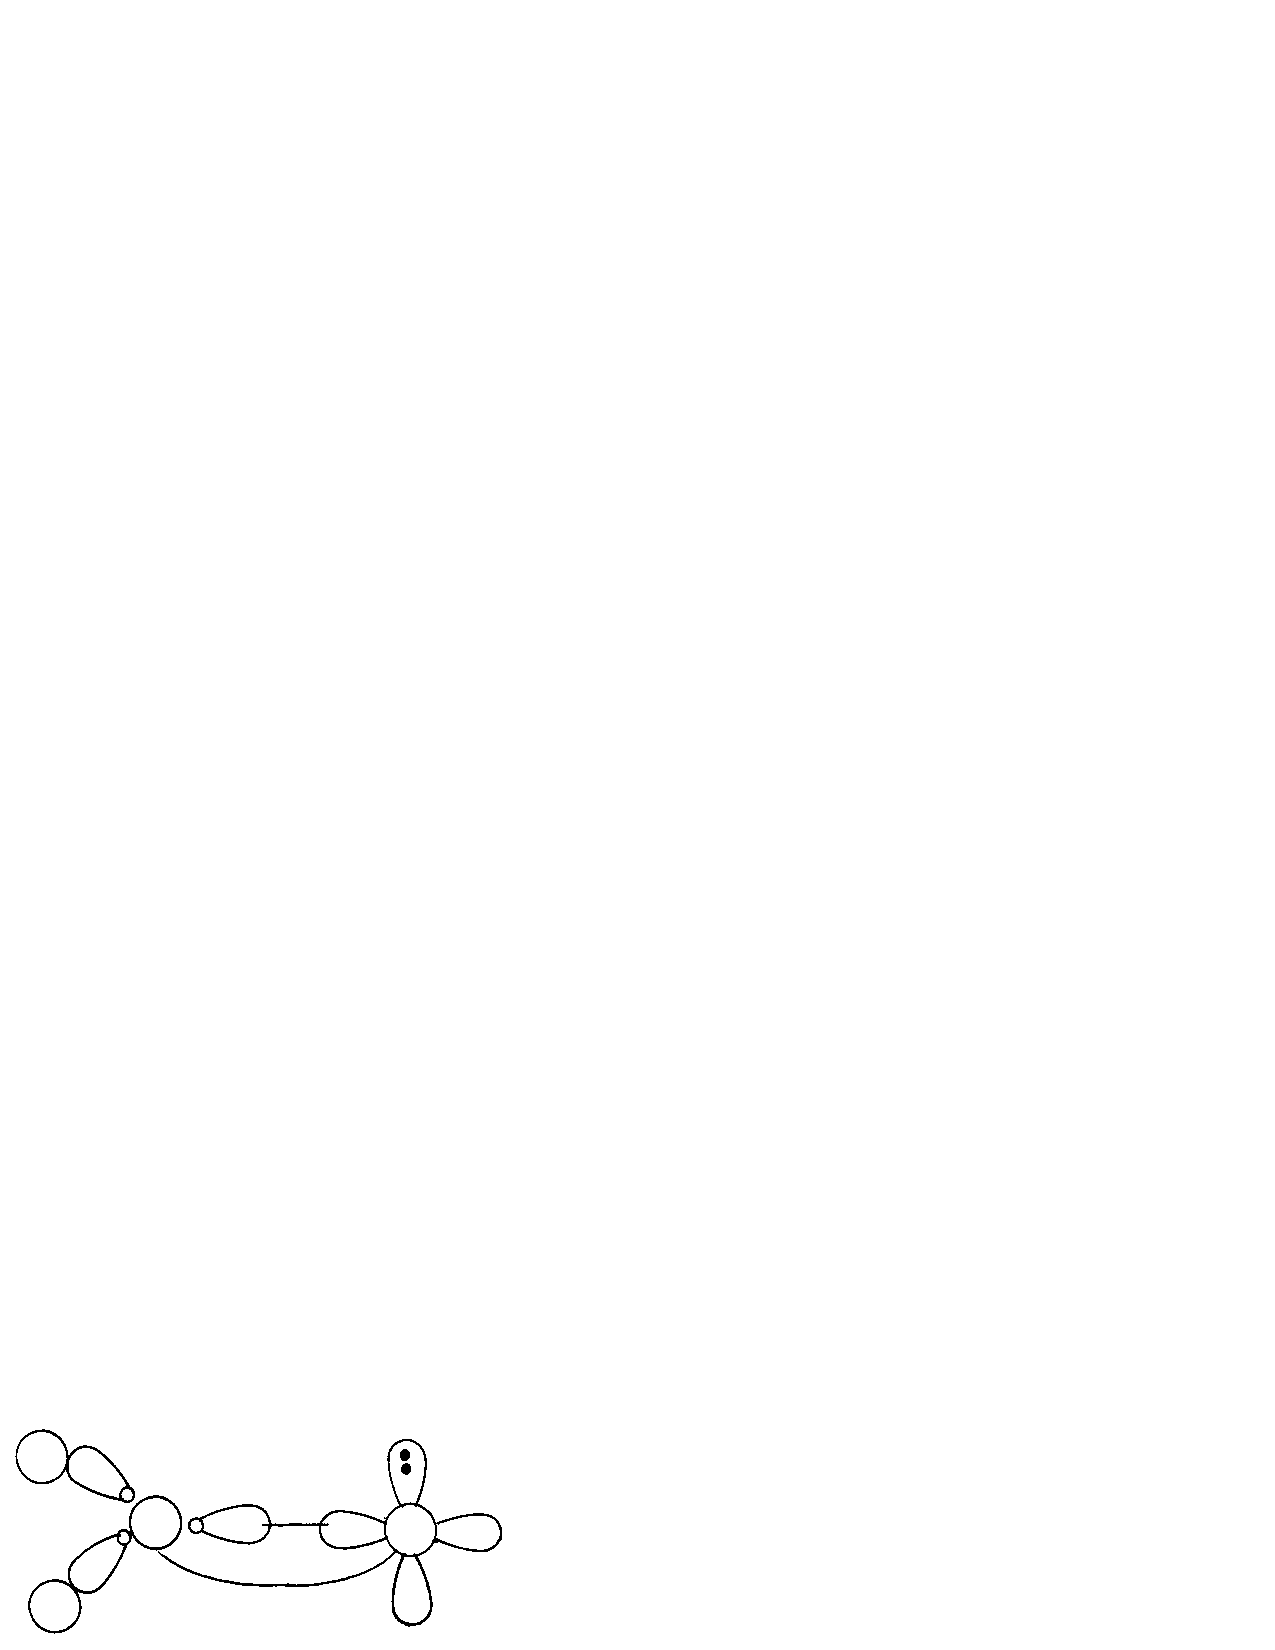
\includegraphics{fg13-6c}
\end{equation}
Now it is even less favorable for the O$\pi_x$ pair to delocalize onto the C, 
two bonds in the way, and we expect a slightly larger $r_e$ and a slightly 
lower $\omega_e$, as observed.

\subsection{CO$_2$}


Starting with the ground states of O and CO
\begin{equation}
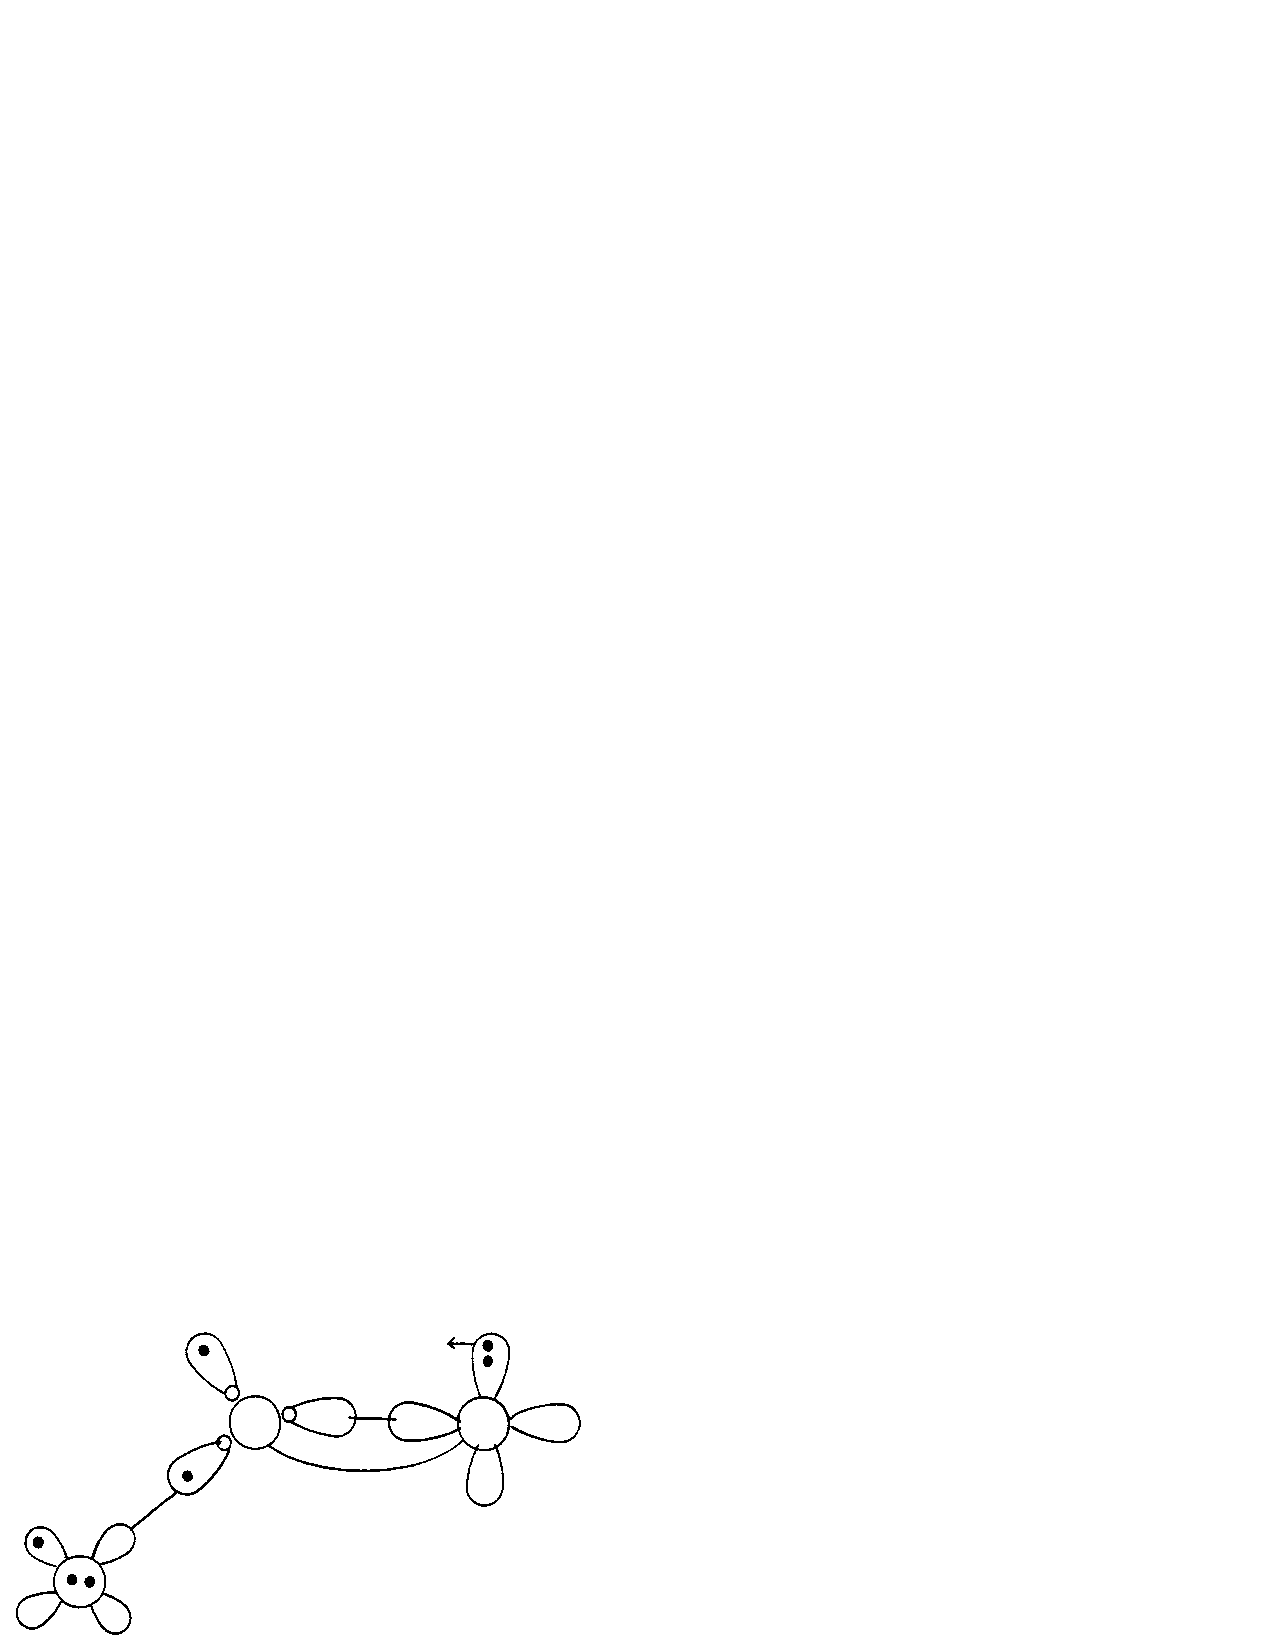
\includegraphics{fg13-6d}
\label{chap13-eqno11}
\end{equation}
we can form a bond as in (\ref{chap13-eqno11}).  However, for the
singlet state, we can also form a bond between the two unpaired
orbitals, leading to
\begin{equation}
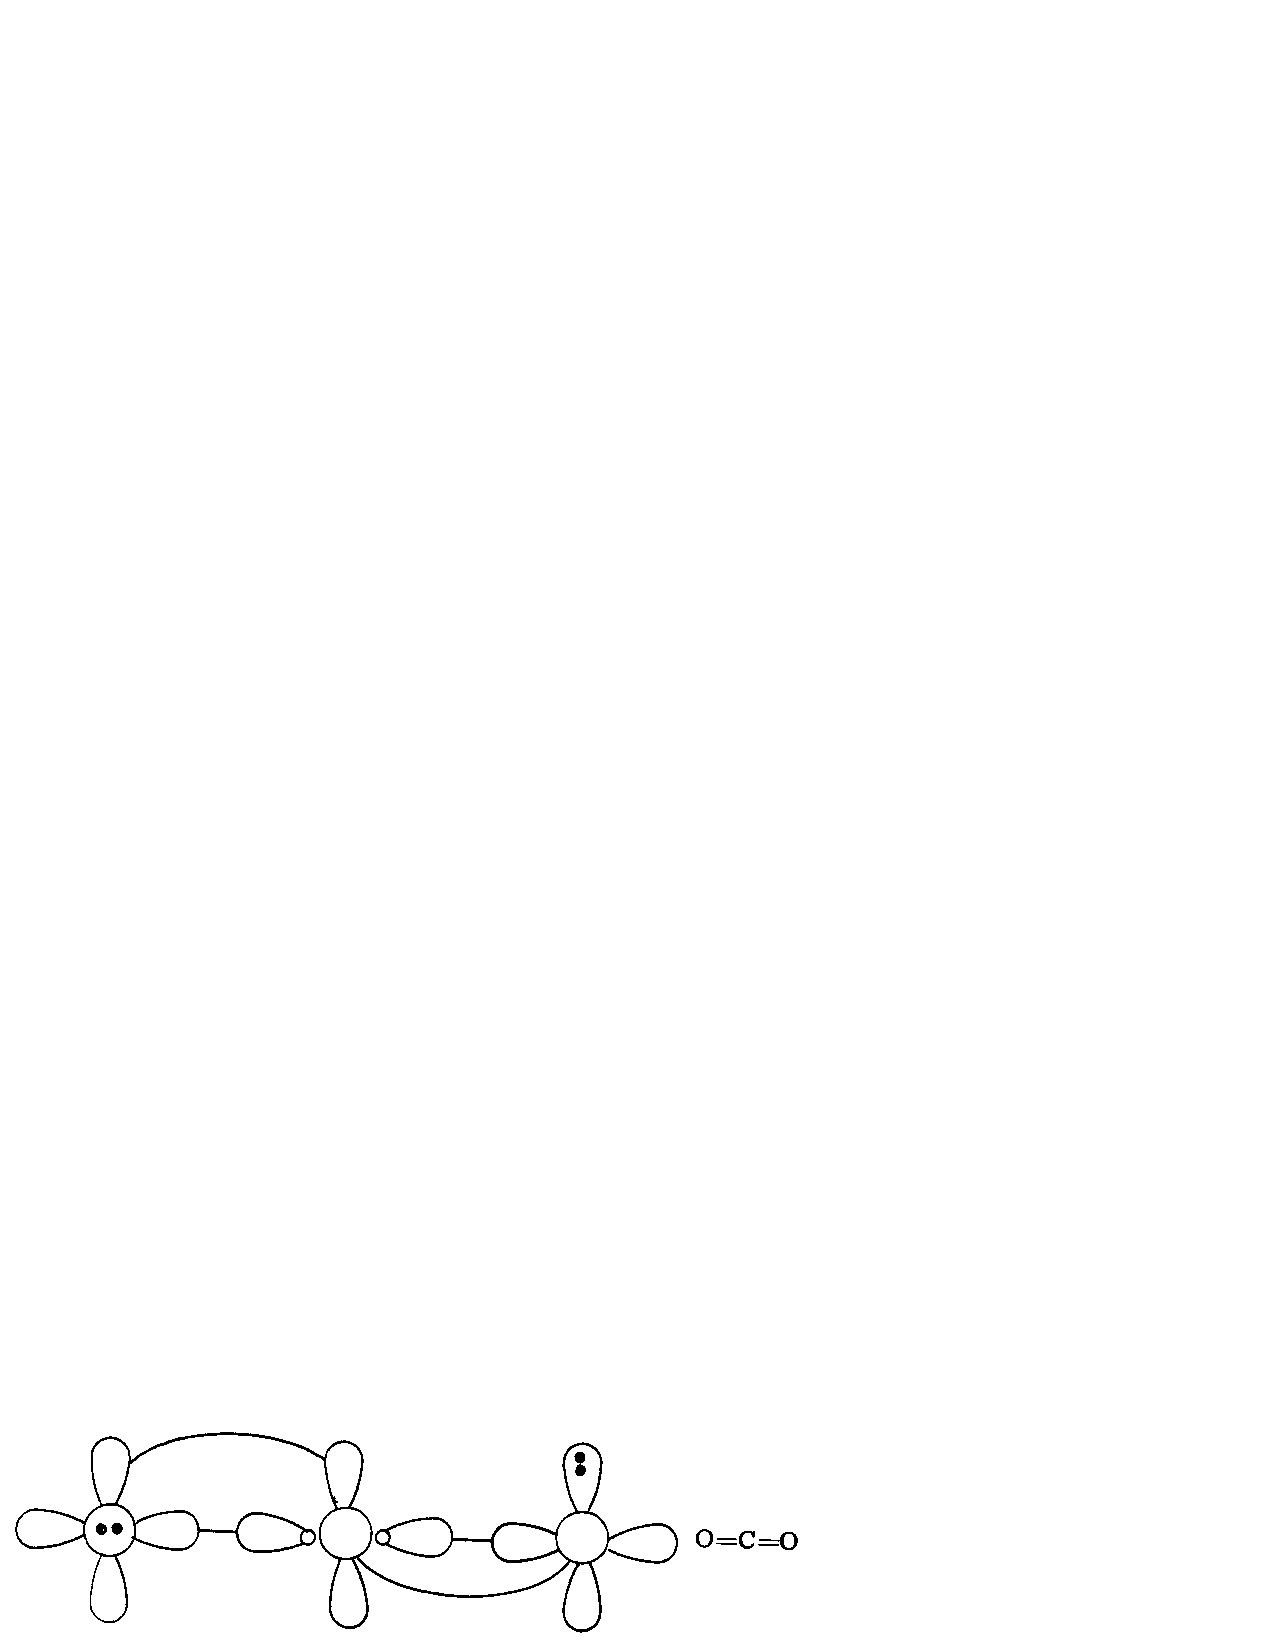
\includegraphics{fg13-6e}
\label{chap13-eqno12}
\end{equation}
linear CO$_2$ with two double bonds.  Actually the pi and sigma bonds
in (\ref{chap13-eqno12}) should be somewhat ionic leading to the
shifts indicated as
\begin{equation}
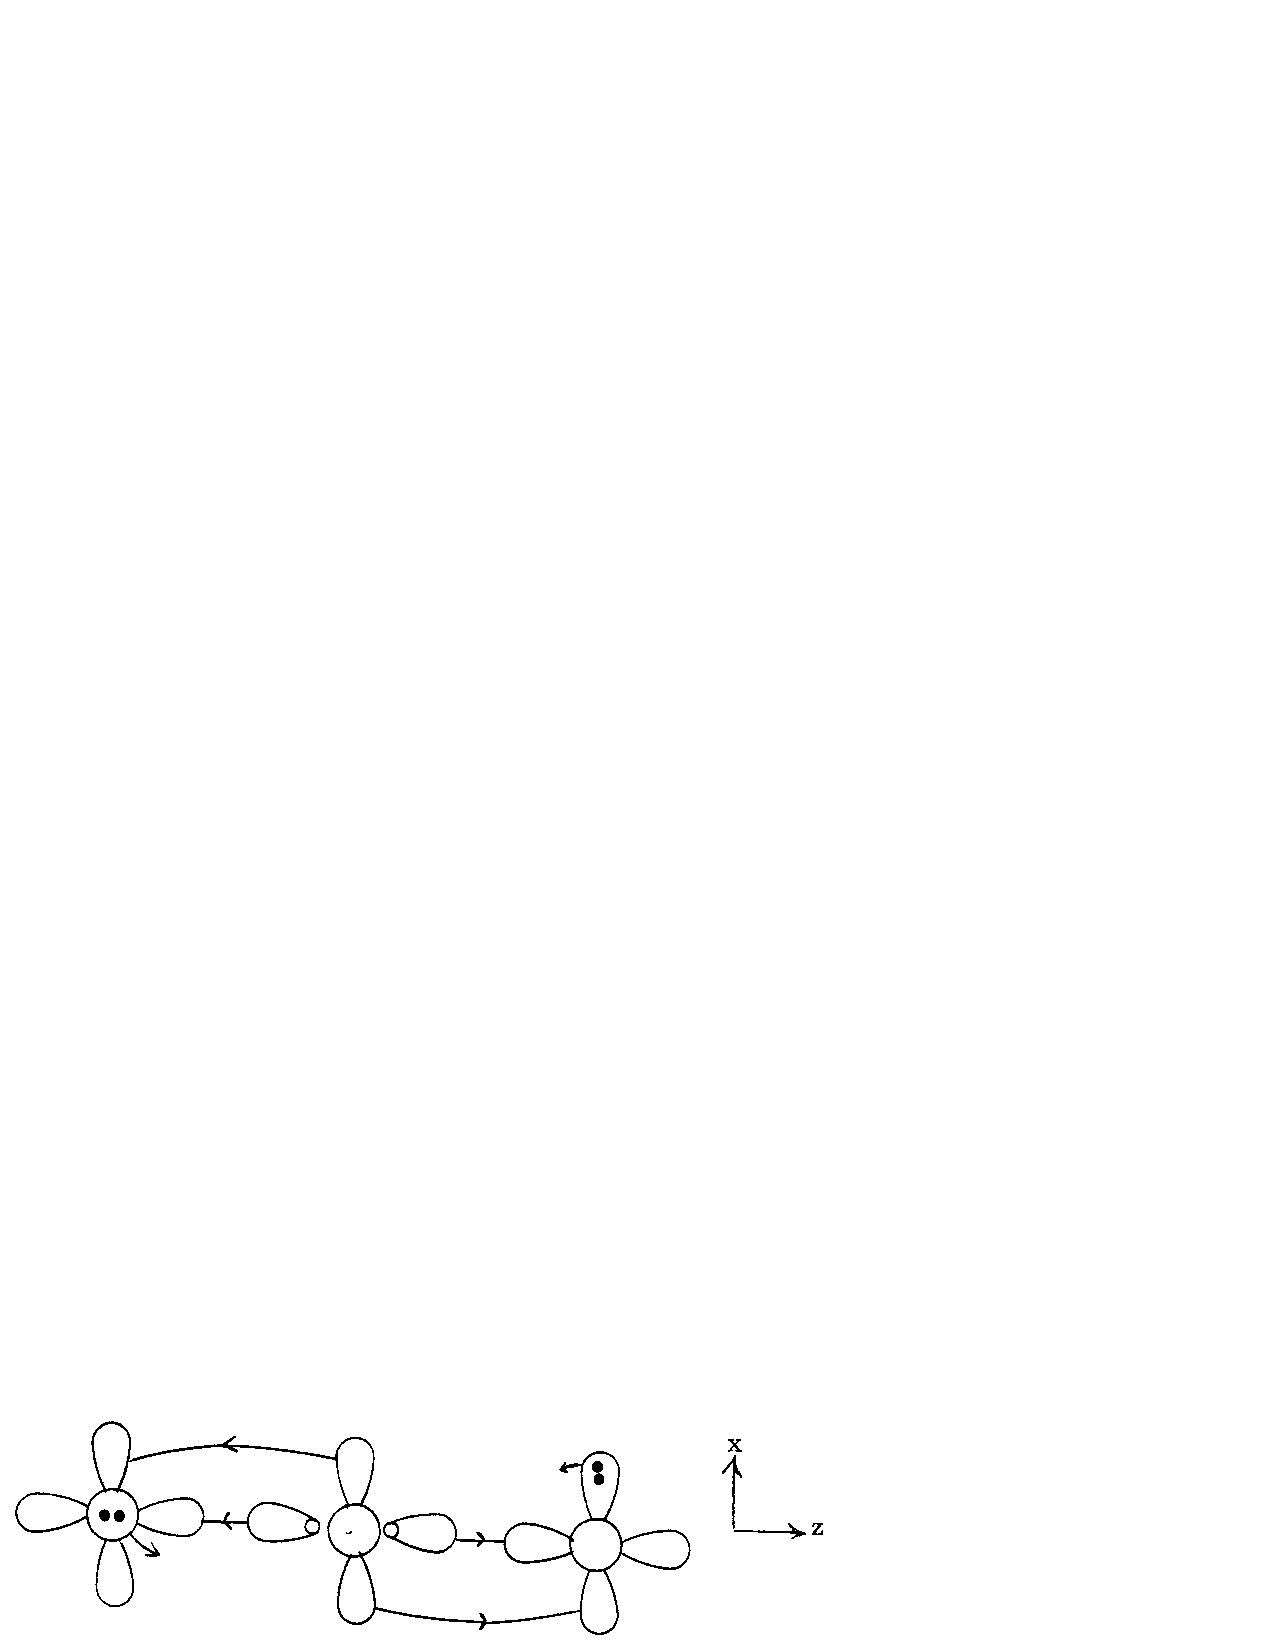
\includegraphics{fg13-6f}
\label{chap13-eqno13}
\end{equation}
by arrows.  Because of the shifts in the bonding orbitals it is
possible for the O$\pi_{xR}$ pairs to shift left, toward the central
C, and for the O$\pi_{yL}$ pair to shift right, toward the central
C. The result is four equivalent pi pairs and ${^1\Sigma}^+_g$
symmetry.  However, we will continue to show the bonding as in
(\ref{chap13-eqno12}) or (\ref{chap13-eqno13}), see Table
\ref{chap13-tab7}.

\begin{table}
\caption{Spectroscopic data for CO$_2$ and C$_3$O$_2$.}
\label{chap13-tab7}
\begin{tabular}{cccccccc}\\ \hline
& & $T_0$ & $r_{0C}$  & OCO & IP & $\nu_{CO}$ & $\nu_{bond}$\cr
& & (cm$^{-1}$) & (\AA) & & (eV)\cr

CO & X $^1\Sigma^+_g$ & 0 & 1.128 & - & 14.013 & 2169.8\cr
CO$)2$ & X $^1\Sigma^+_g$ & 0$^a$ & 1.1621 & 180$^{\circ}$ & 13.769 & 
1388 & 667\cr
& & & & & & 2349\cr
& A $^1B_2(^1\Delta_u)$ &46000$^b$ & 1.246 & 122 $\pm$ 2\cr
C$_3$O$_2$ & X $^1\Sigma^+_g$ & 0 & - & -\cr
& A & 30697 & - & 180$^{\circ}$\cr
\hline
\end{tabular}\\
$^a$D(O-CO) = 5.453 eV>
$^b$Next state at 71000 cm$^{-1}$.
\end{table}

The low-lying excited states of CO$_2$ are derived from
(\ref{chap13-eqno11}) and (\ref{chap13-eqno14})
\begin{equation}
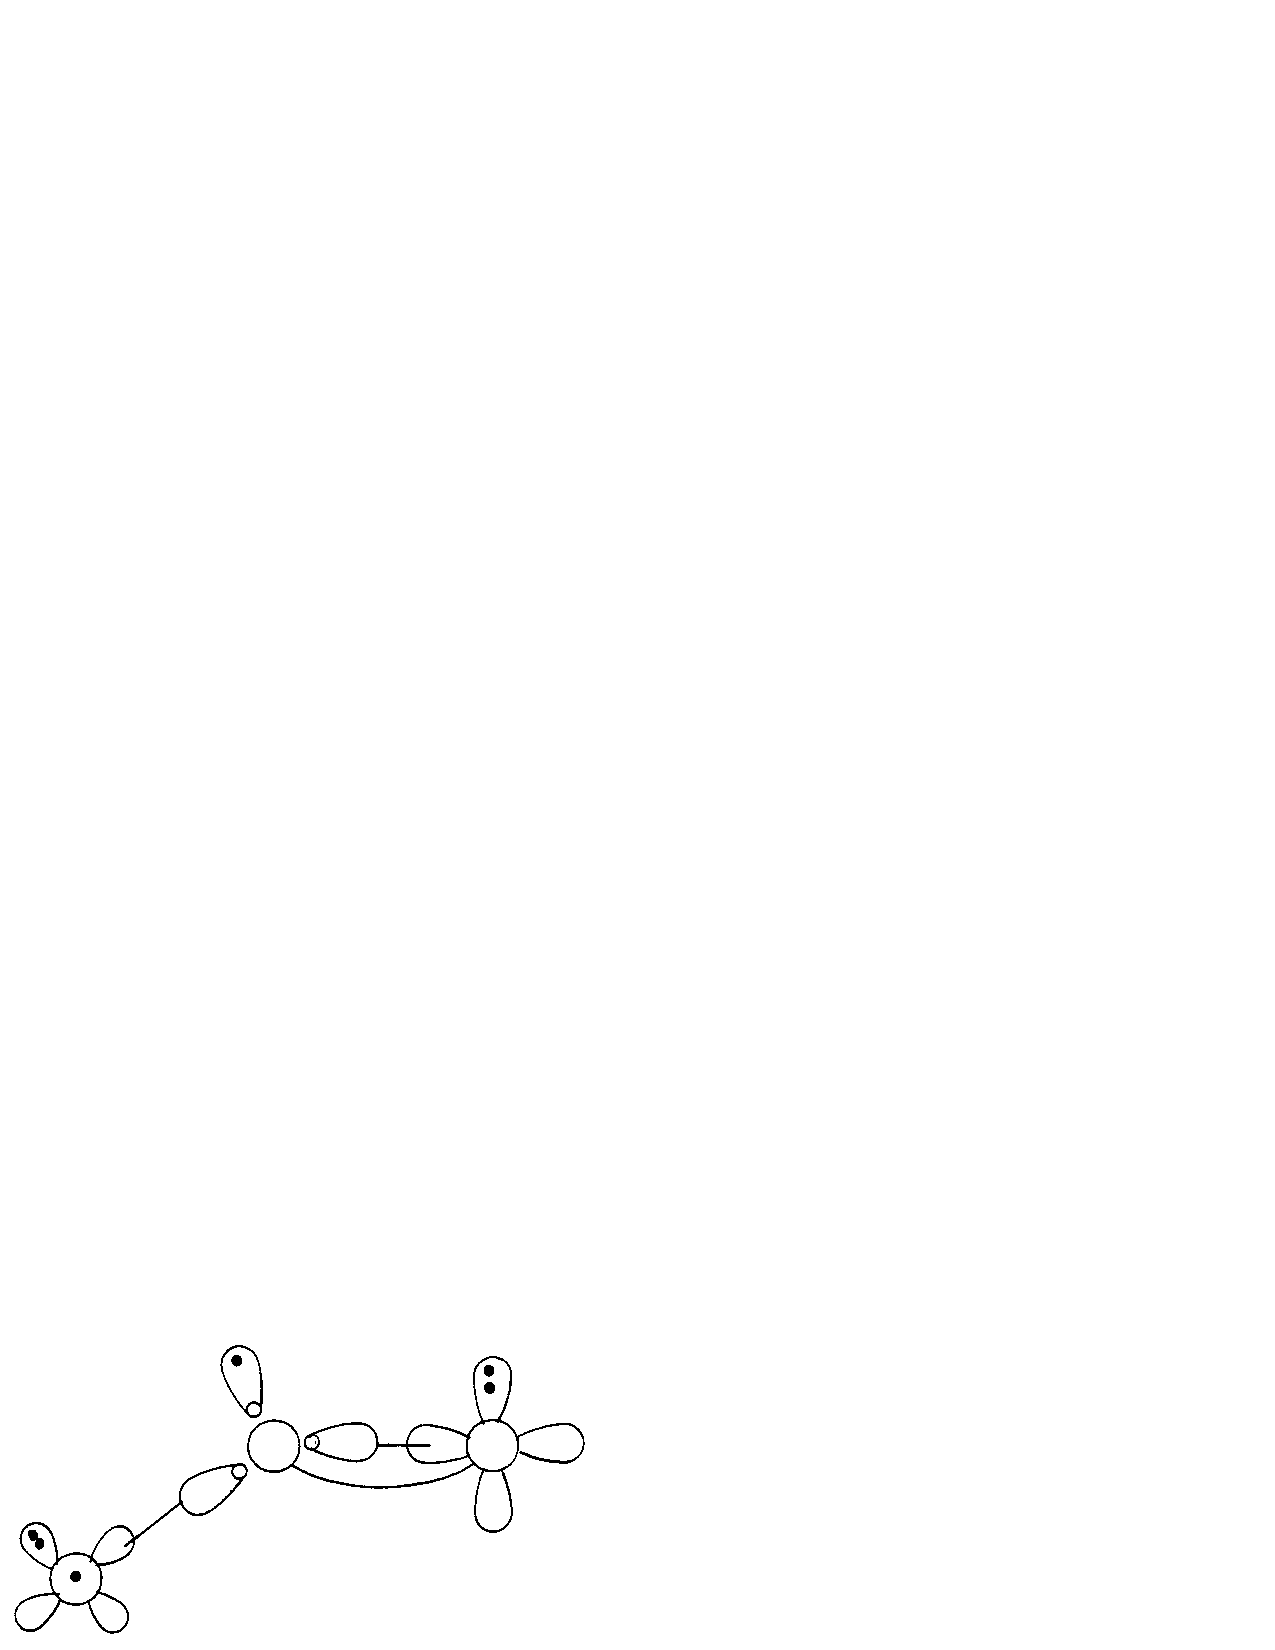
\includegraphics{fg13-6g}
\label{chap13-eqno14}
\end{equation}
Besides the ground state, (\ref{chap13-eqno11}) leads to ${^3B}_2$,
${^1B}_2$, and ${^3A}_1$ states, and (\ref{chap13-eqno14}) leads to
${^3A}_2$, ${^1A}_2$, ${^3B}_1$, and ${^1B}_1$ states.  Note that
(\ref{chap13-eqno11}) and (\ref{chap13-eqno12}) each represent two
configurations, one with the excitation on the left and one with it on
the right.  These seven states should all have bent geometries. Only
one has been found experimentally, see Table \ref{chap13-tab7}, but
recent calculation$^1$ show all seven to have vertical excitation
energies of 6 to 10 eV.

In (\ref{chap13-eqno11}), we can shift the Op$\pi$ to the carbon,
leading to
\begin{equation}
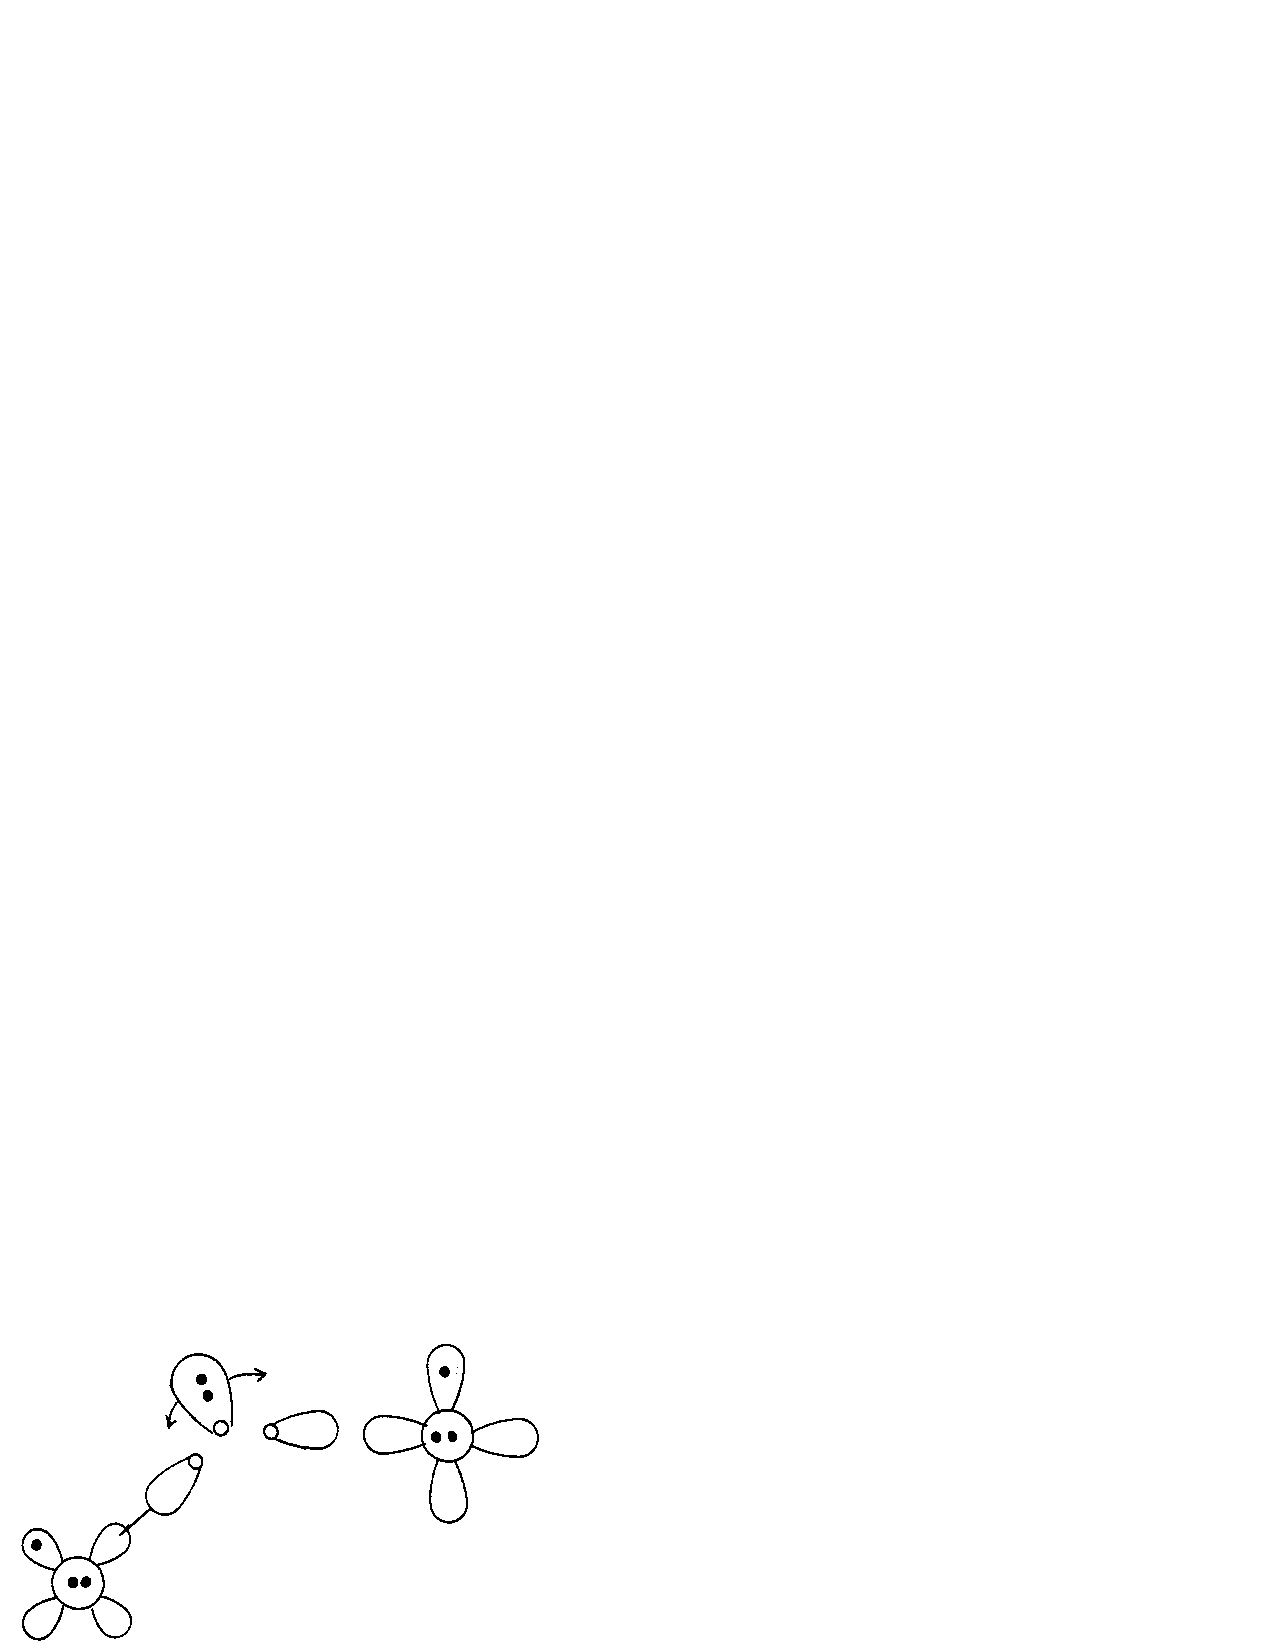
\includegraphics{fg13-6h}
\label{chap13-eqno15}
\end{equation}
Configuration (\ref{chap13-eqno15}) leads to a singlet state,
${^1A}_1$
\begin{equation}
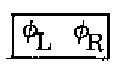
\includegraphics{fg13-6i-1}
\end{equation}
and a triplet state, ${^3B}_2$
\begin{equation}
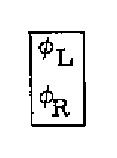
\includegraphics{fg13-6i-2}
\end{equation}
Since the orbitals are overlapping, the singlet state should be lower
with the ${^1A}_1 - {^3B}_2$ splitting energy depending upon the
$\langle \phi_{\ell} | \phi_r \rangle$ overlap.  The arrows in
(\ref{chap13-eqno15}) indicate that the nonbonding pair in the C
delocalized onto the neighboring Os. This leads to an increased
overlap between the $\phi_L$ and $\phi_R$ orbitals, since they each
must be orthogonal to the delocalized C pair.

As a result, the ${^1A}_1 {^3B}_2$ separation is 1.2 eV at 120
degrees.  However, from (\ref{chap13-eqno15}) we see that the $\phi_L$
and $\phi_R$ orbitals can overlap on the back side, leading to a sigma
bond and a small bond angle
\begin{equation}
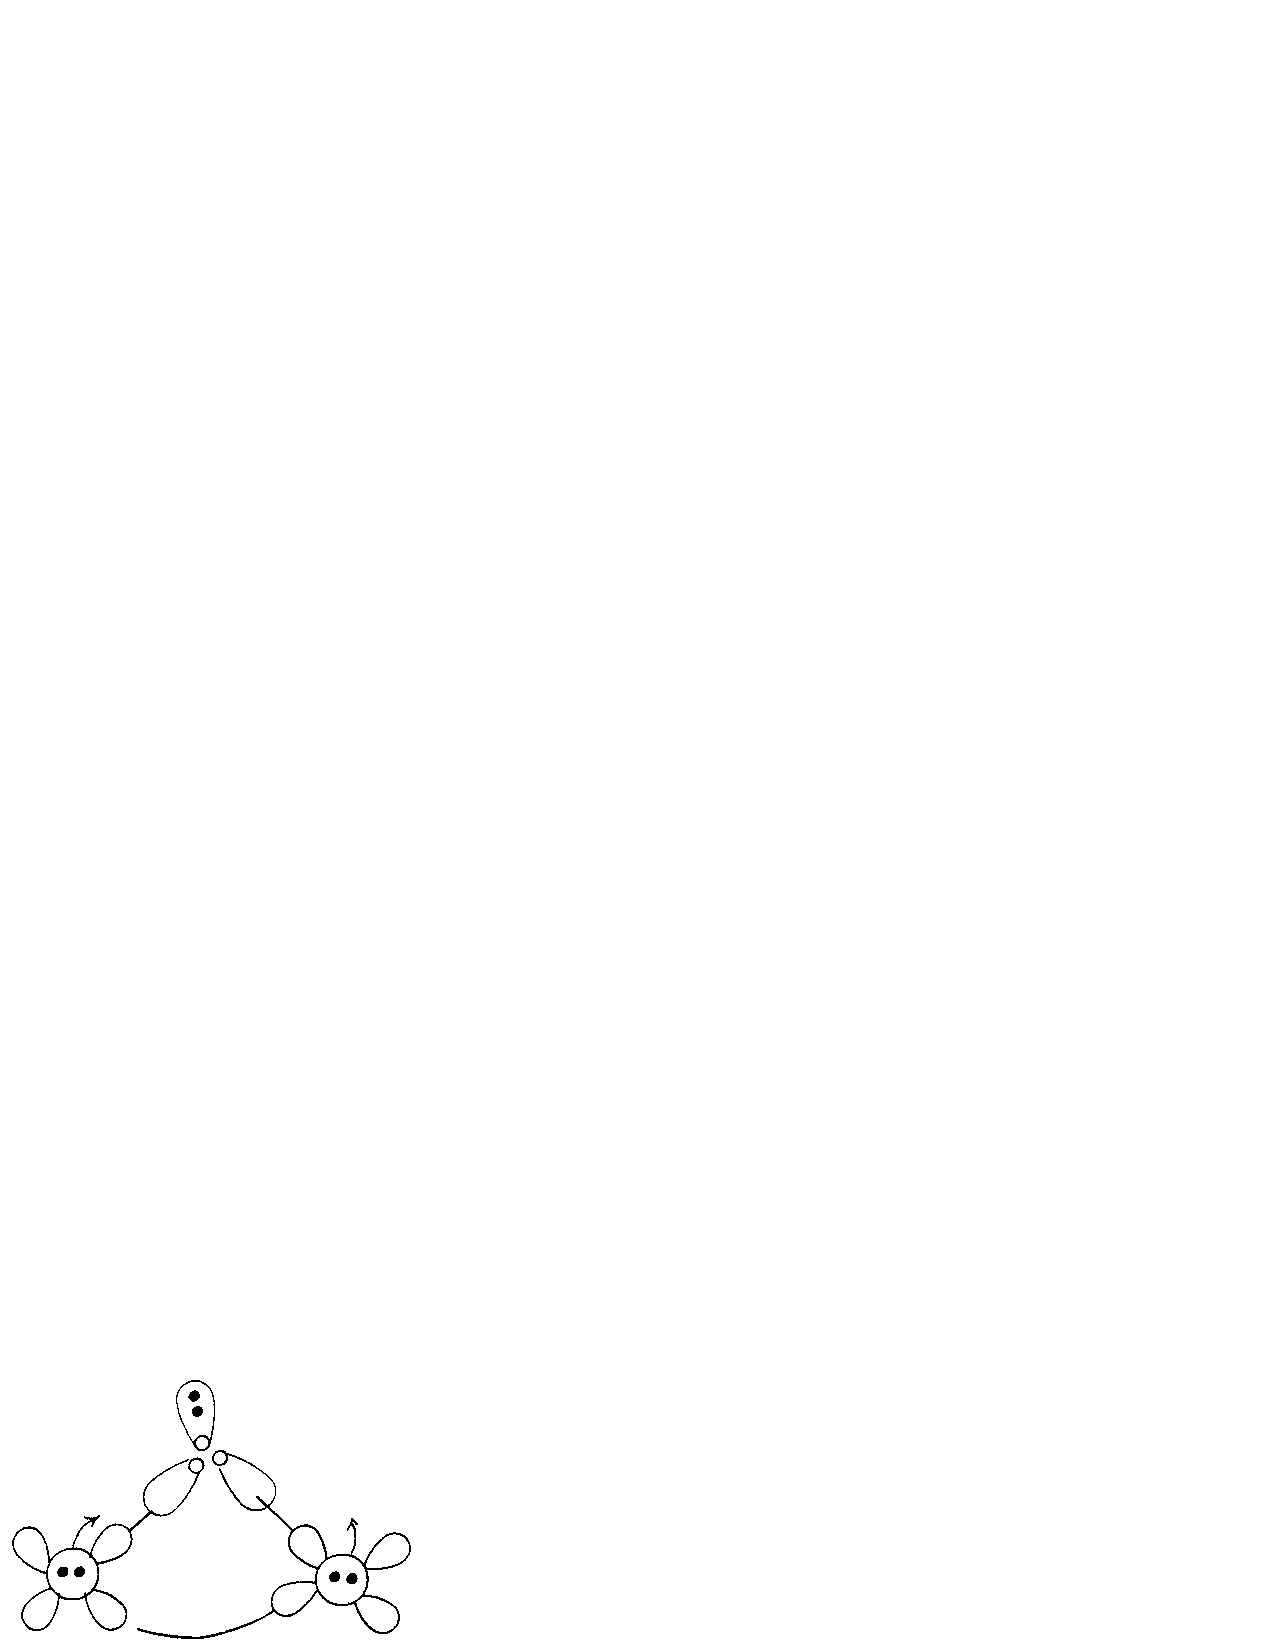
\includegraphics{fg13-6j}
\end{equation}
This state would be higher than the ground state (\ref{chap13-eqno12})
of CO$_2$, but might be lower than the bent molecule in
(\ref{chap13-eqno15}).  In this case, the ground potential curve for
CO$_2$ would have a double minimum.

\begin{figure}
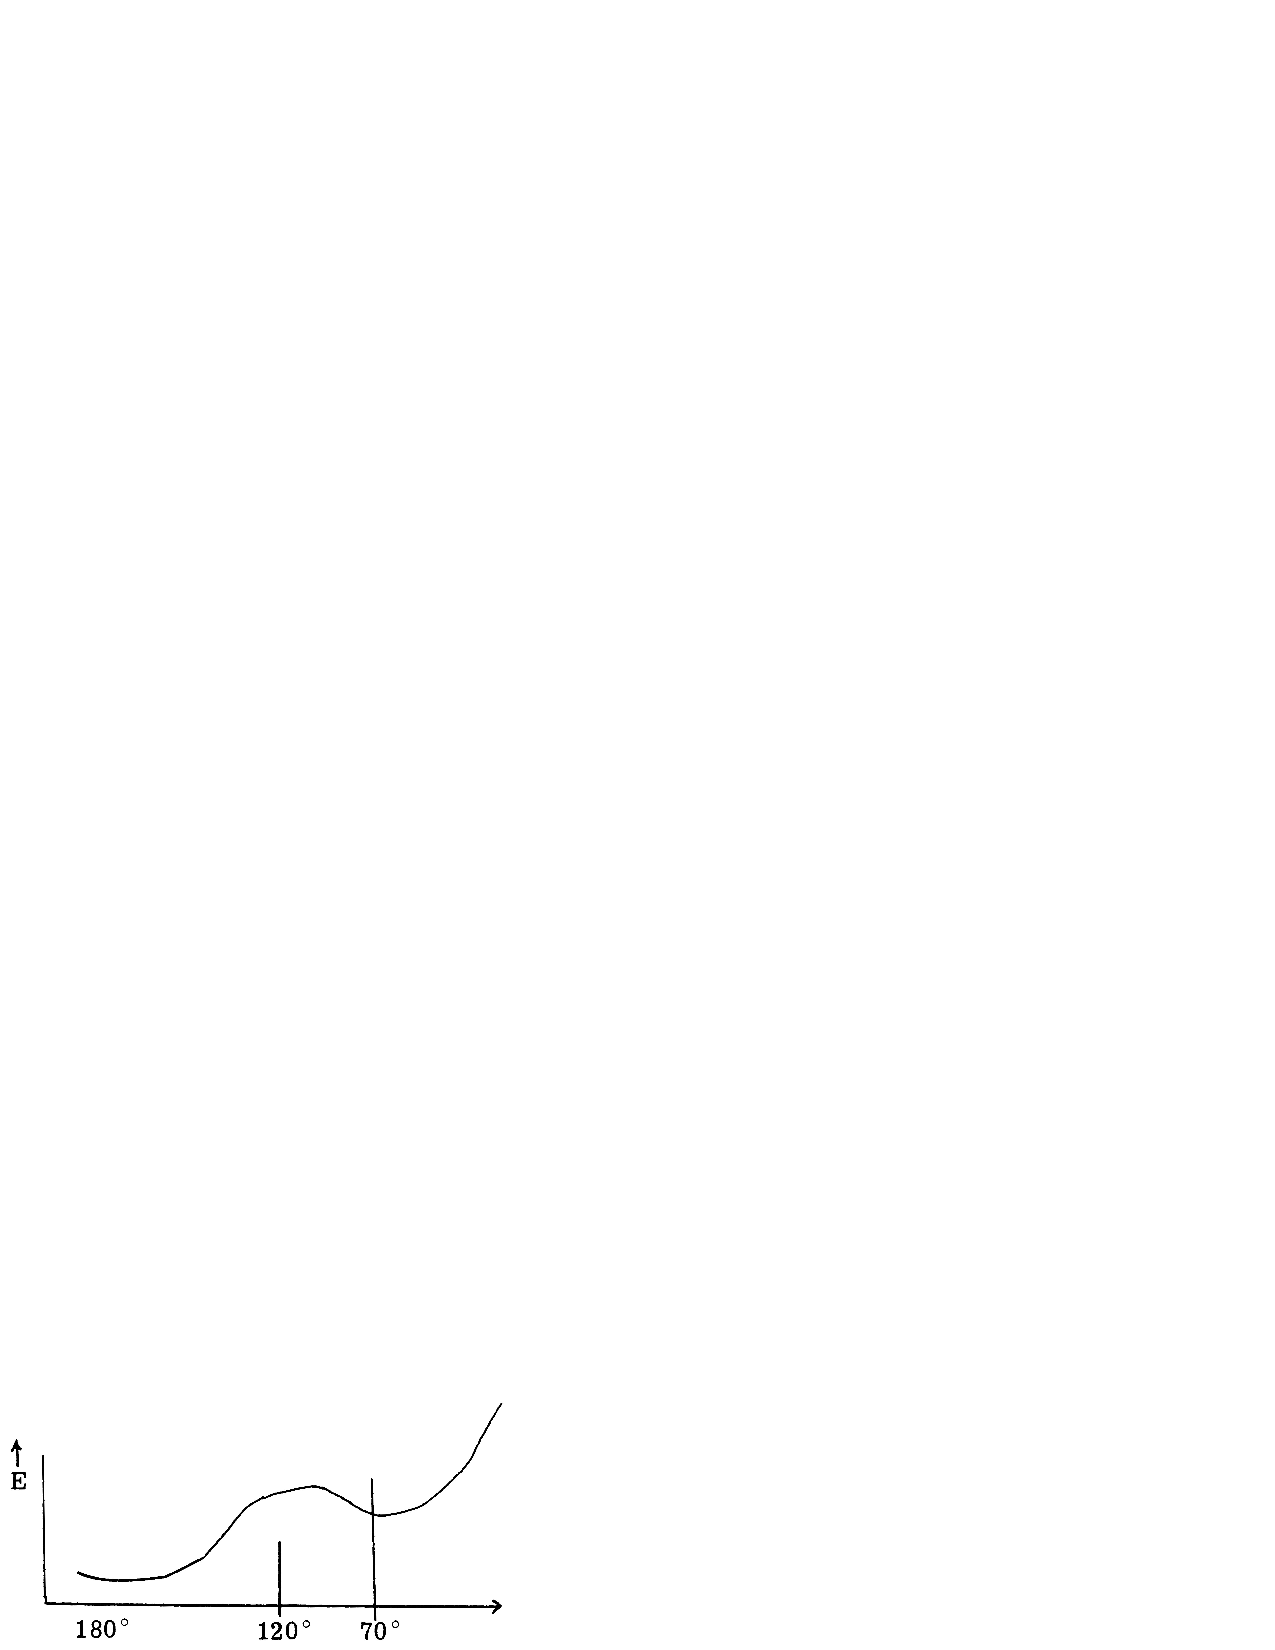
\includegraphics[scale=0.75]{fg13-7}
\caption{}
\label{chap13-fig7}
\end{figure}

\subsection{Carbon Suboxide}

Starting with (\ref{chap13-eqno12}), we might try building O = C = C =
O and O = C = C = C = O, etc.  For C$_2$O$_2$ we find the bonding to
be
\begin{equation}
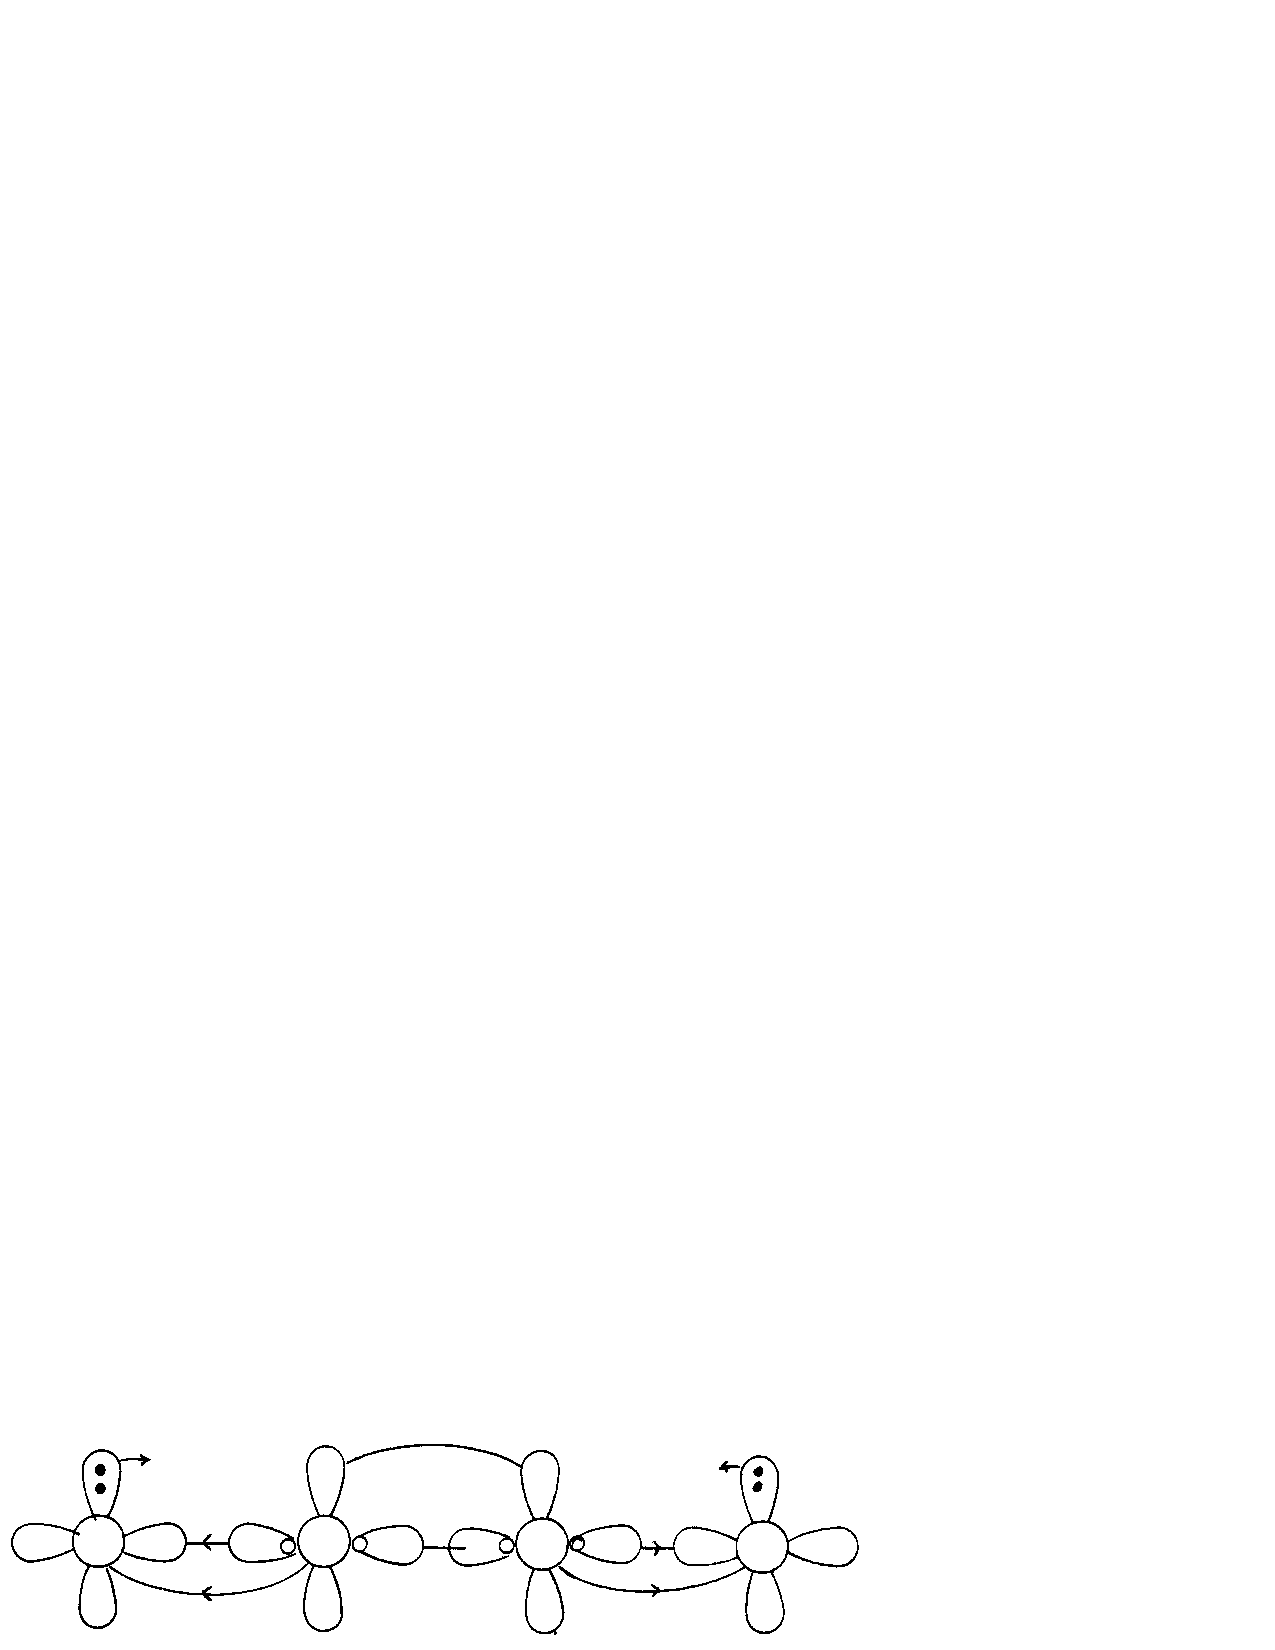
\includegraphics{fg13-7a}
\end{equation}
We have put in arrows to show the ionic character of the bonds. In the case 
of CO$_2$, the ionic character of the pi bonds leads to changes in concert 
with the delocalization of the O$\pi$ pairs.  However, this does not occur 
for C$_2$O$_4$.

On the other hand, for C$_3$O$_2$, carbon suboxide, the bonding is
\begin{equation}
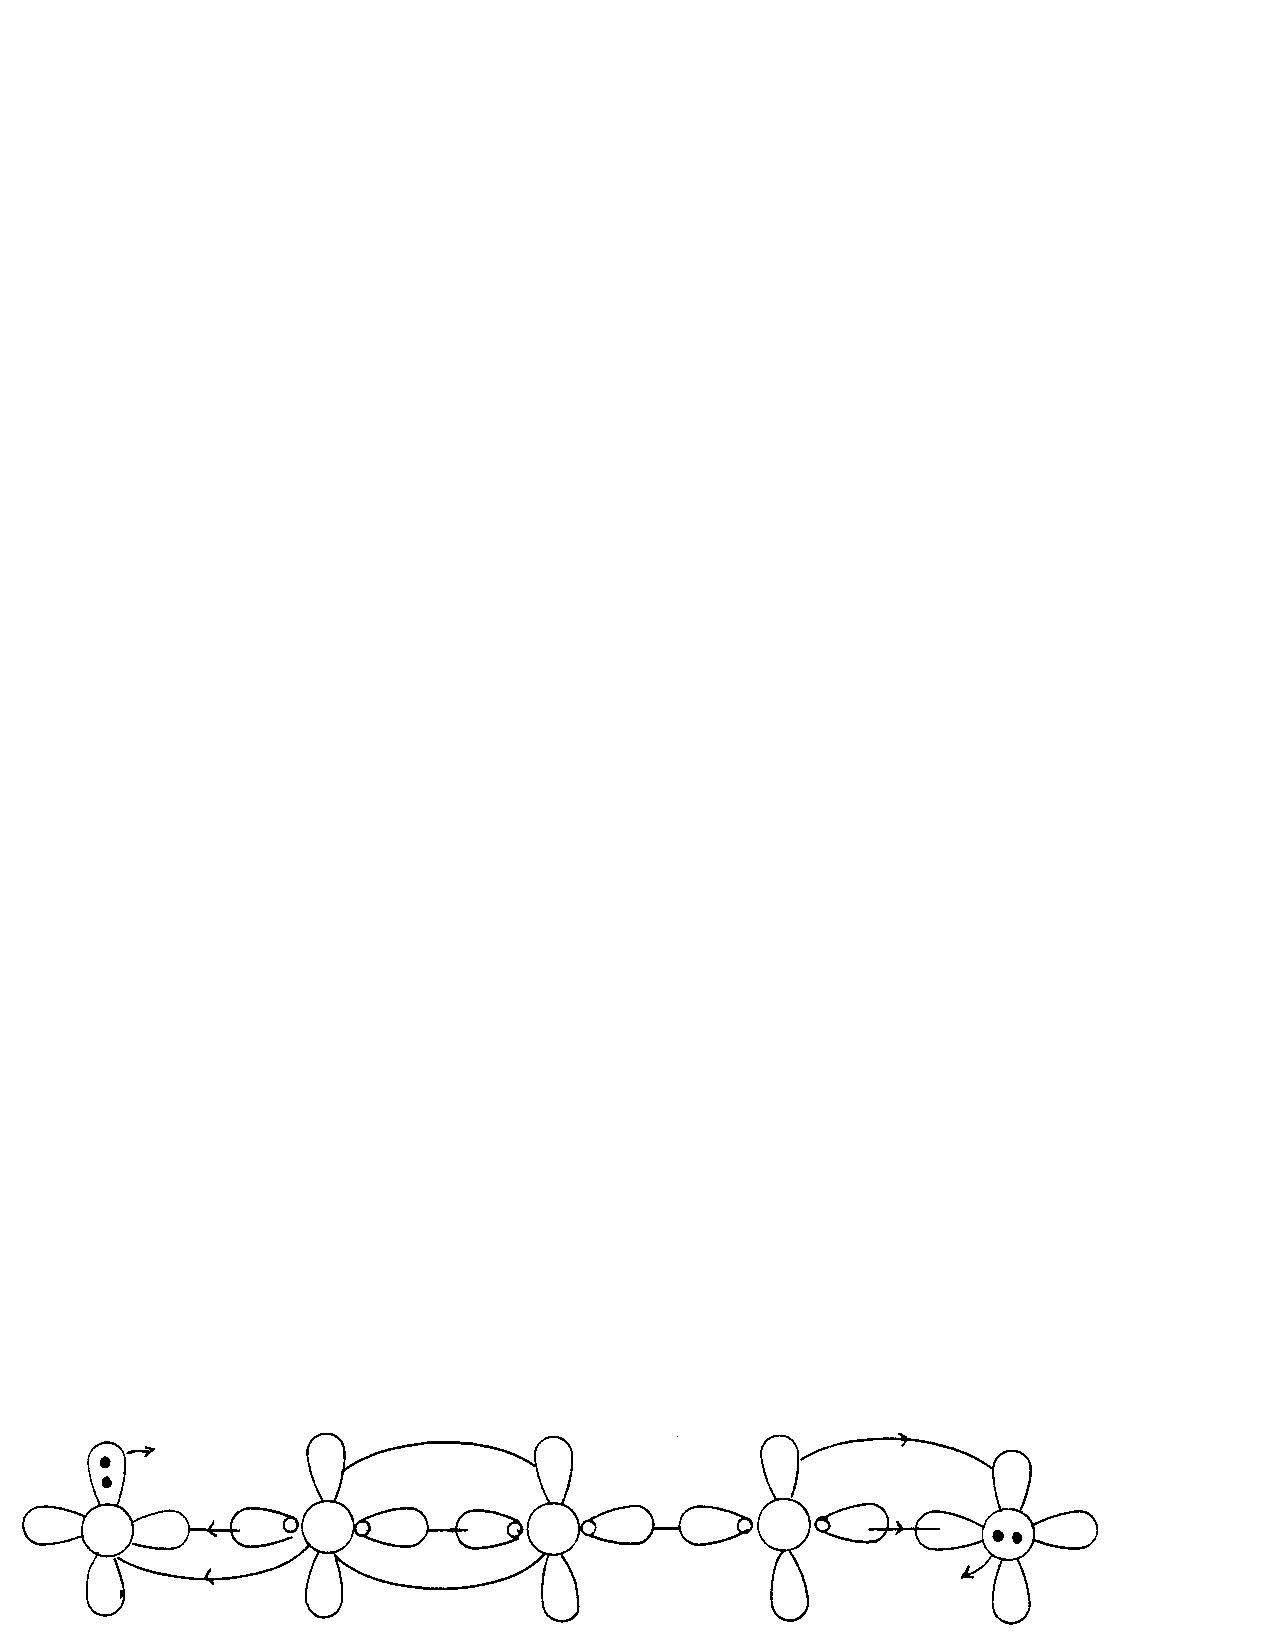
\includegraphics{fg13-7b}
\end{equation}
so that all $\pi_x$ pairs shift to the right, while all $\pi_y$ pairs shift to 
the left.  As a result, we expect stronger bonding for C$_3$O$_1$, and 
other even carbon chains.  This is in agreement
with C$_3$O$_2$ being a commonly observed species, while C$_2$O$_2$ is not known.

Dissociating C$_3$O$_2$ leads to CO + C$_2$O with the latter having the bonding
\begin{equation}
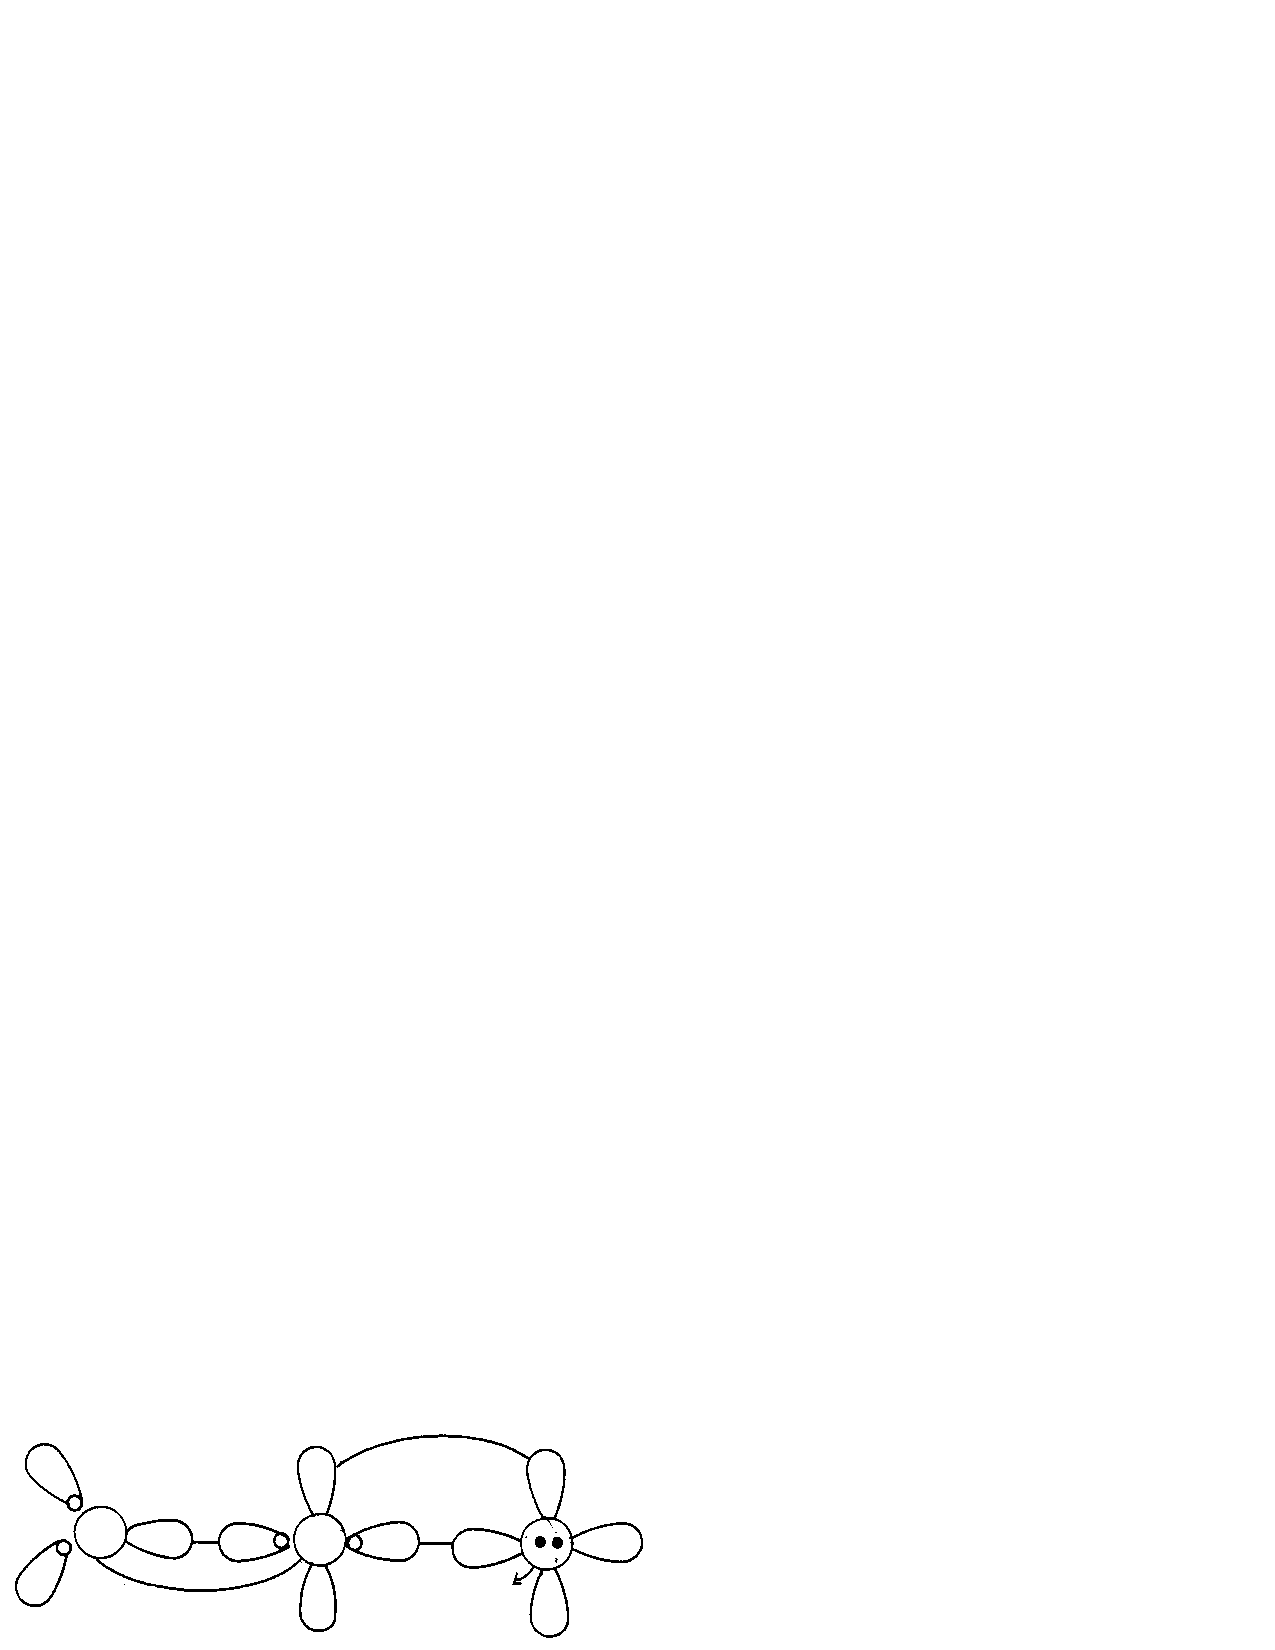
\includegraphics{fg13-7c}
\end{equation}
a ${^1\Sigma}^+_g$ state, or
\begin{equation}
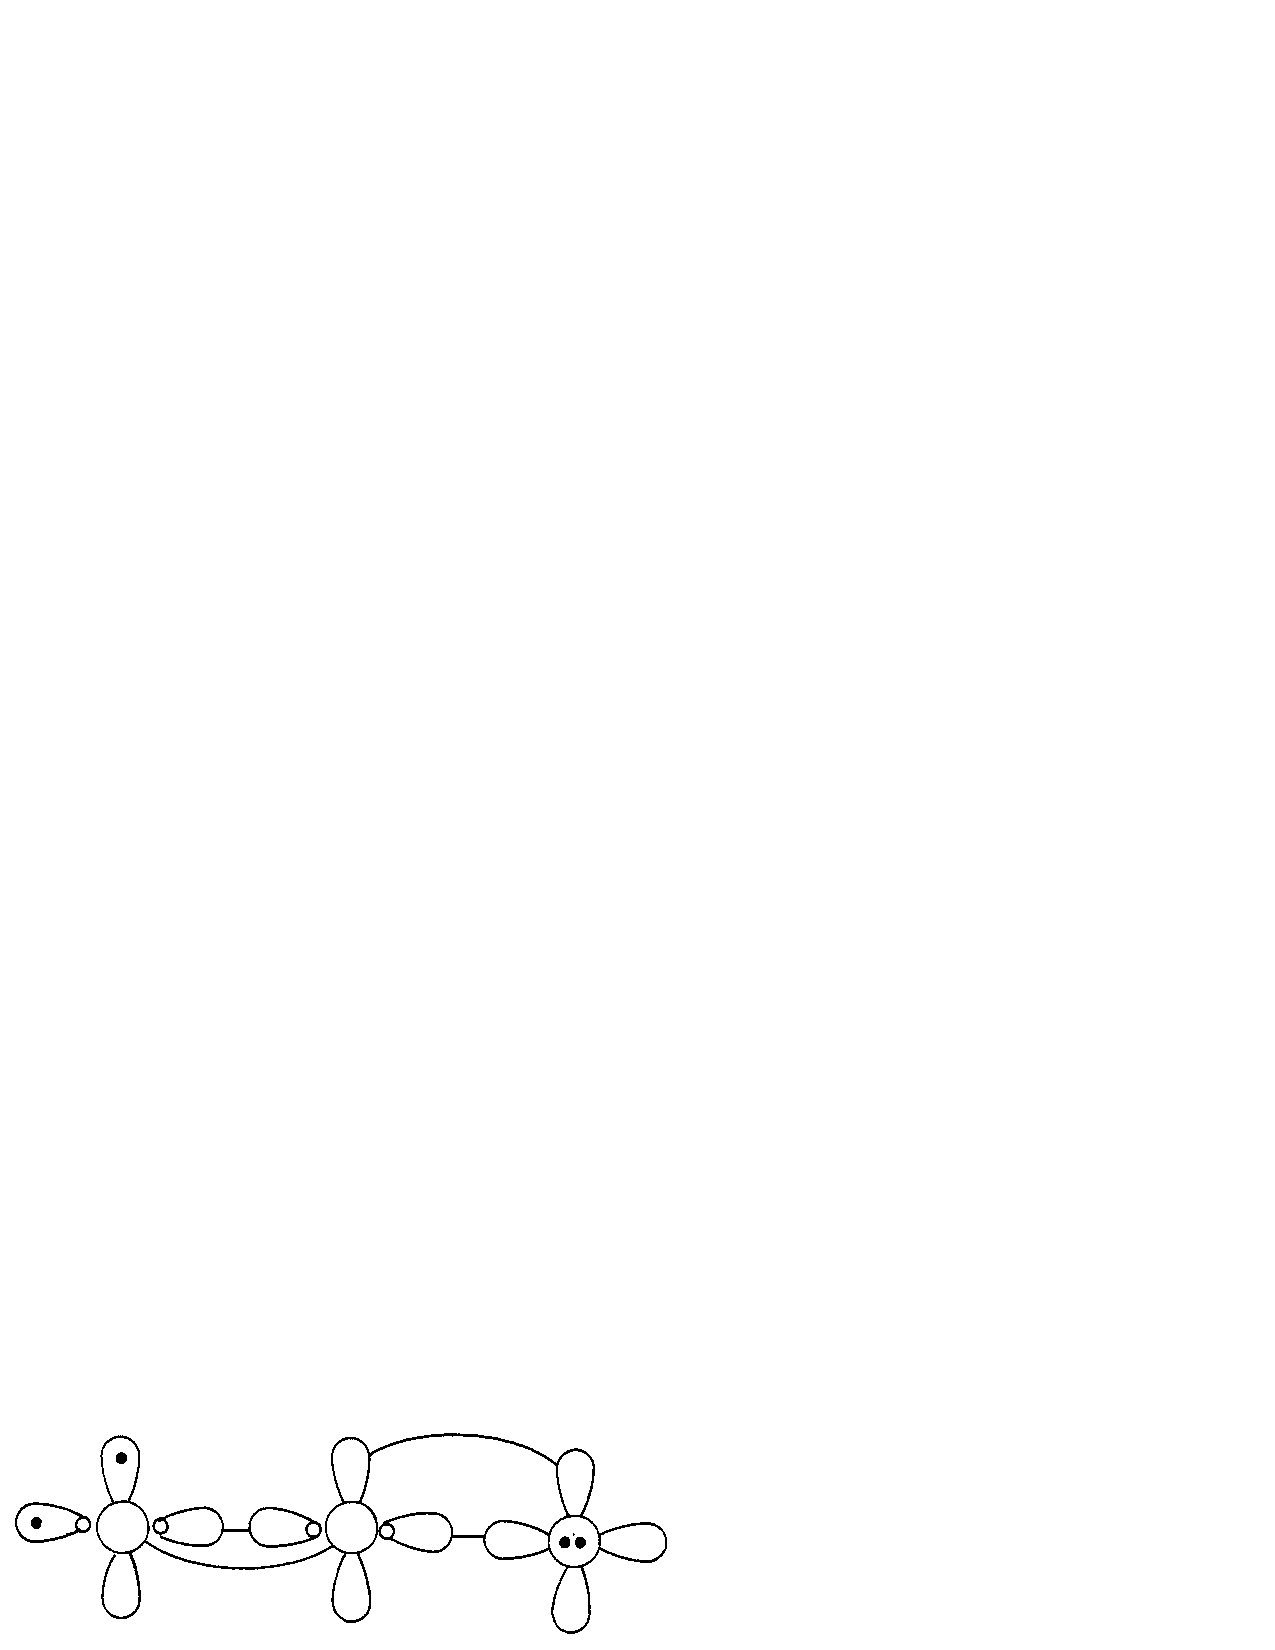
\includegraphics{fg13-7d}
\end{equation}
a${^3\Pi}$ or ${^1\Pi}$ state.

\section{NO}

Starting with the ground states of the atoms, we expect NO to have the 
bonding
\begin{equation}
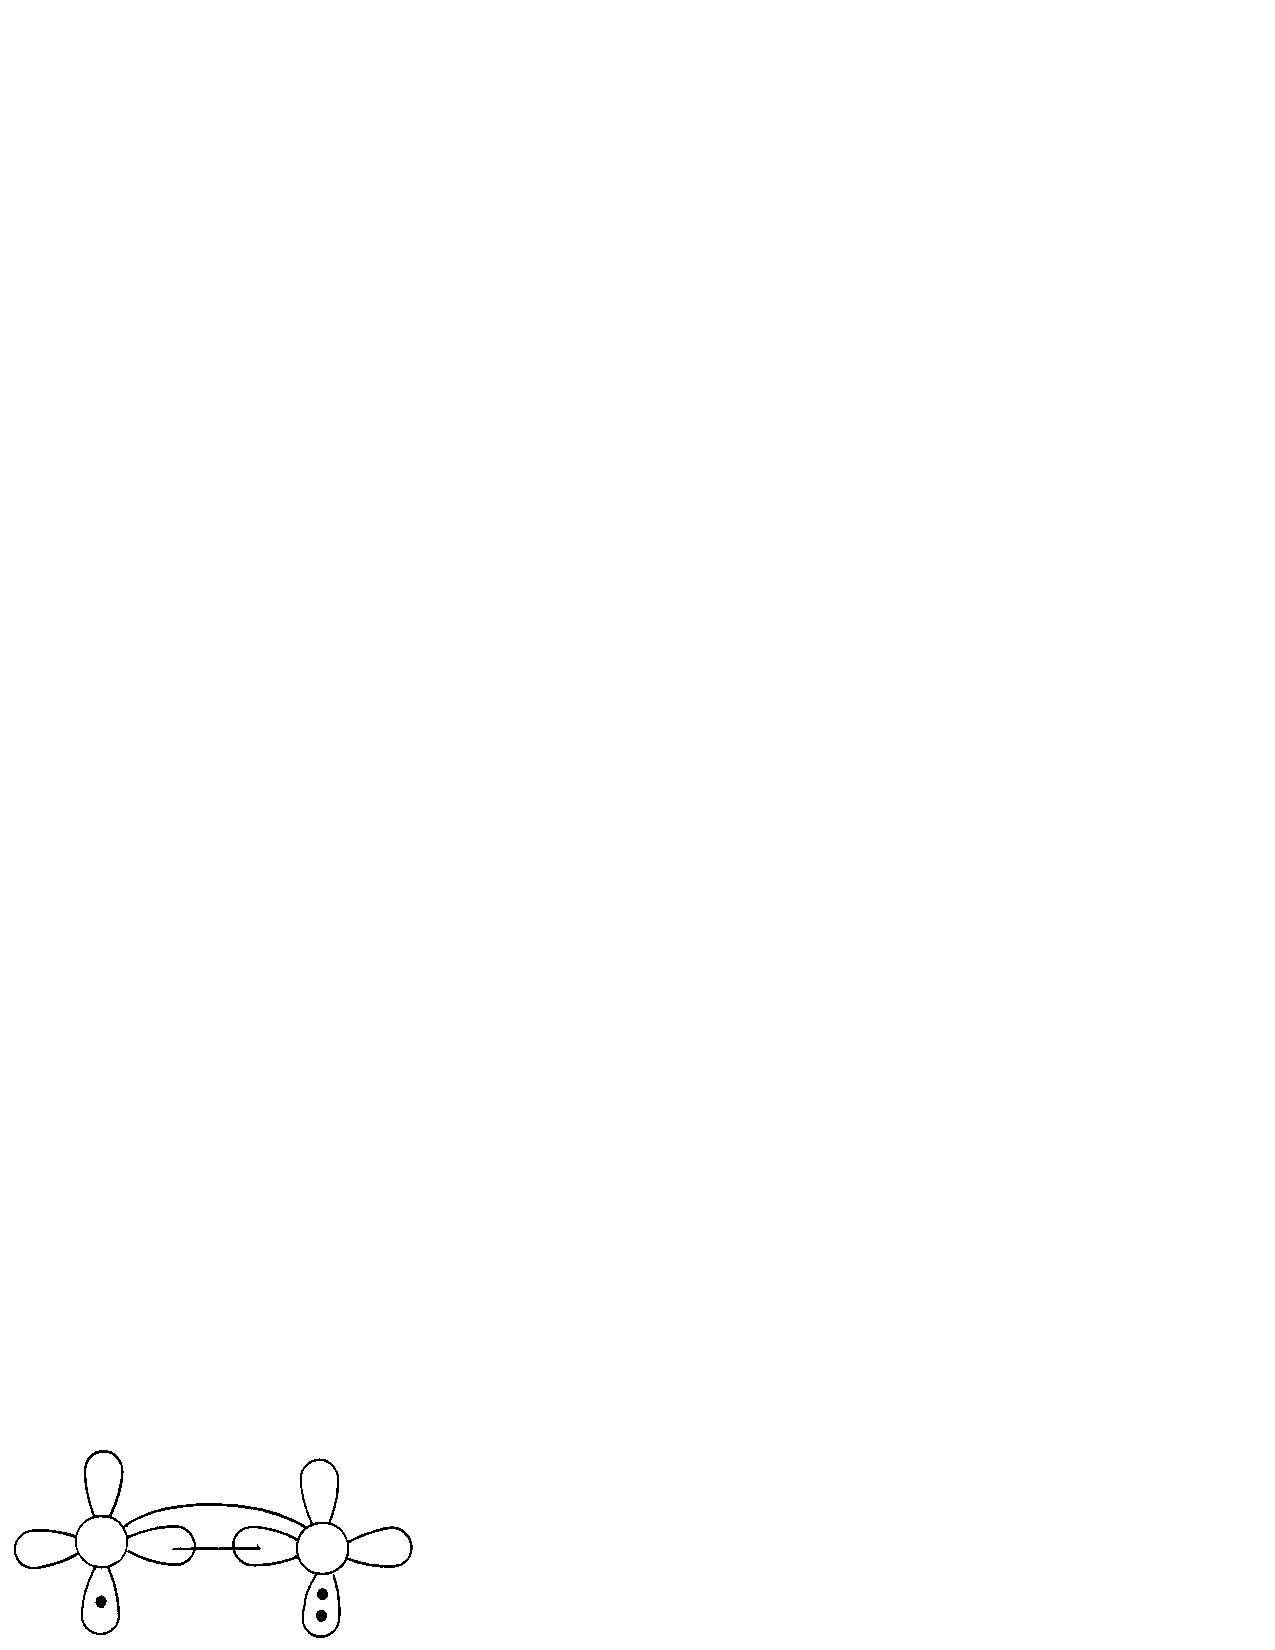
\includegraphics{fg13-7e}
\end{equation}
leading to a ${^2\Pi}$ state.  Just as in O$_2$, the $\pi_x$ orbital 
on the N here should be highly antibonding.  Removing it leads to 
NO$^+$
\begin{equation}
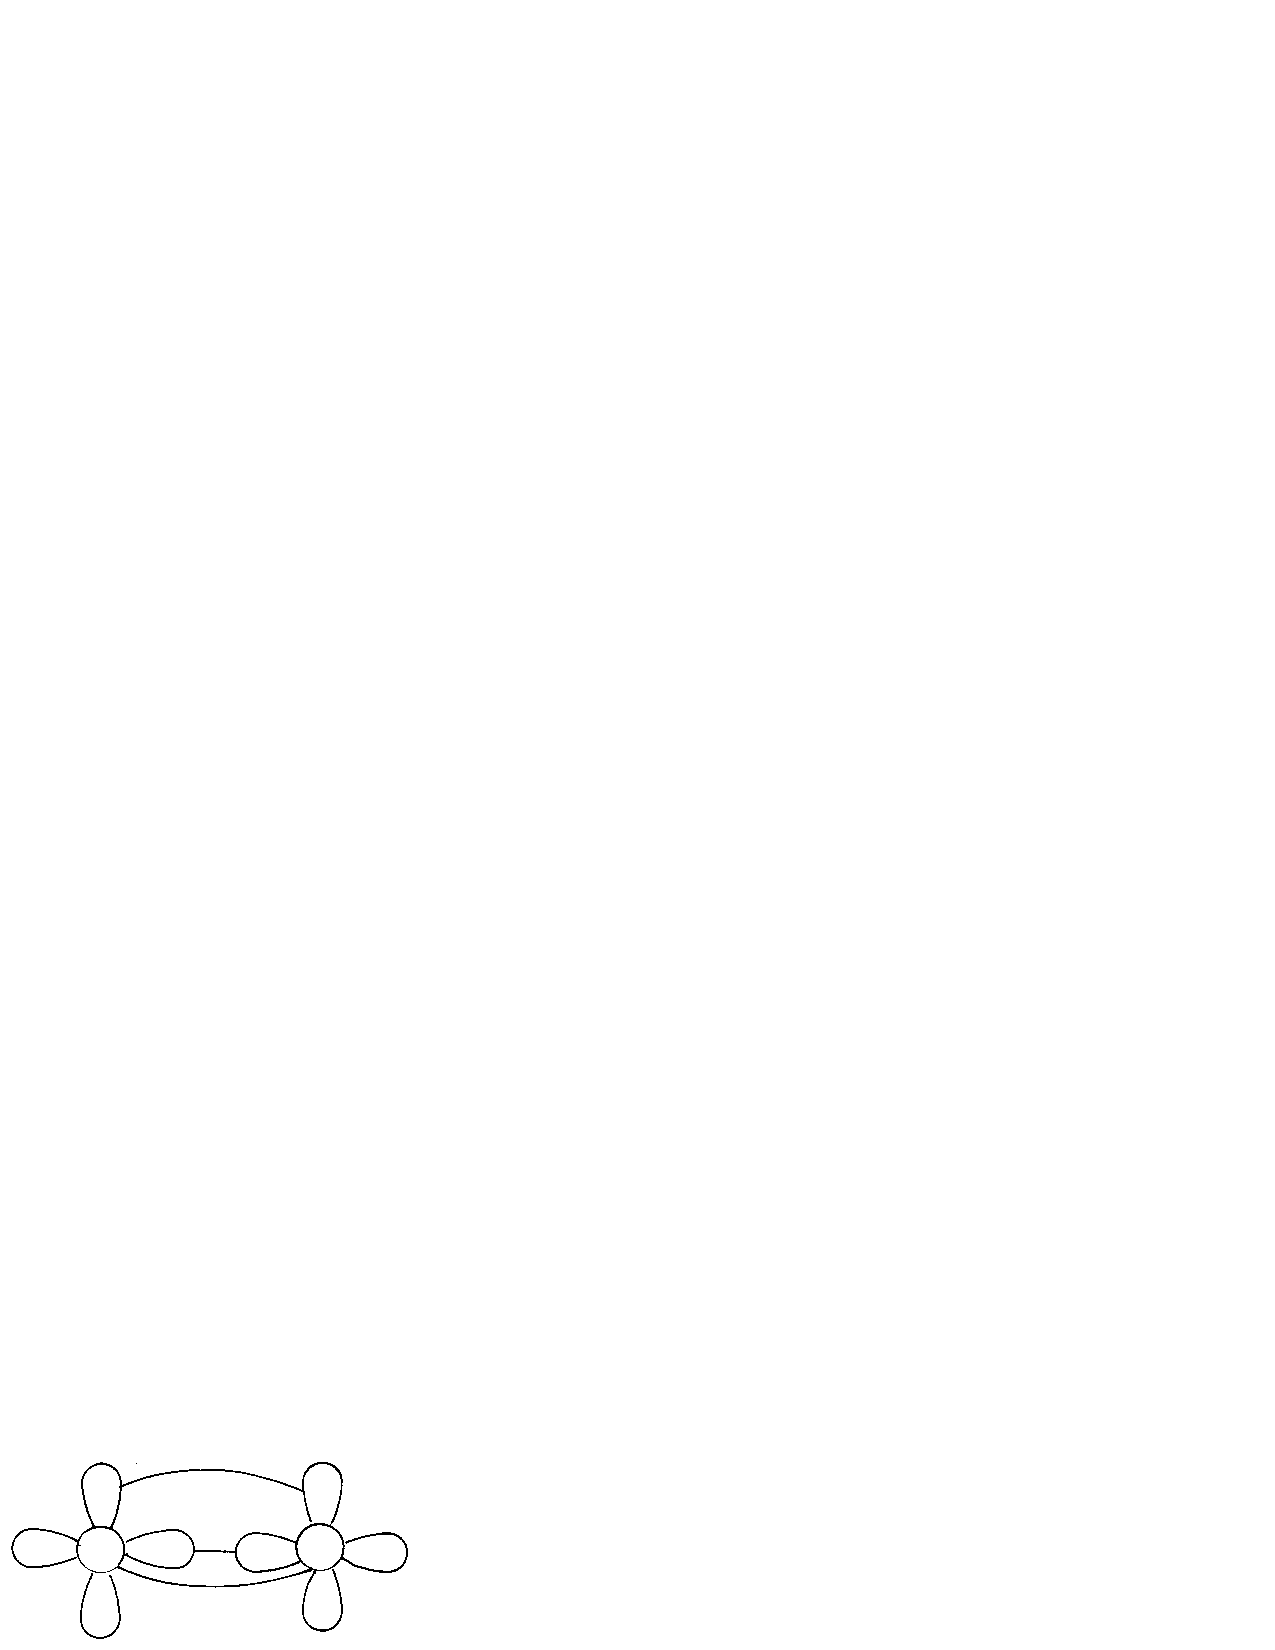
\includegraphics{fg13-7f}
\end{equation}
which should have a very strong bond.  Thus, the Rydberg states of NO should 
have shorter bond lengths than the ground state.

Other states of NO can be obtained from N($^2$P)
\begin{equation}
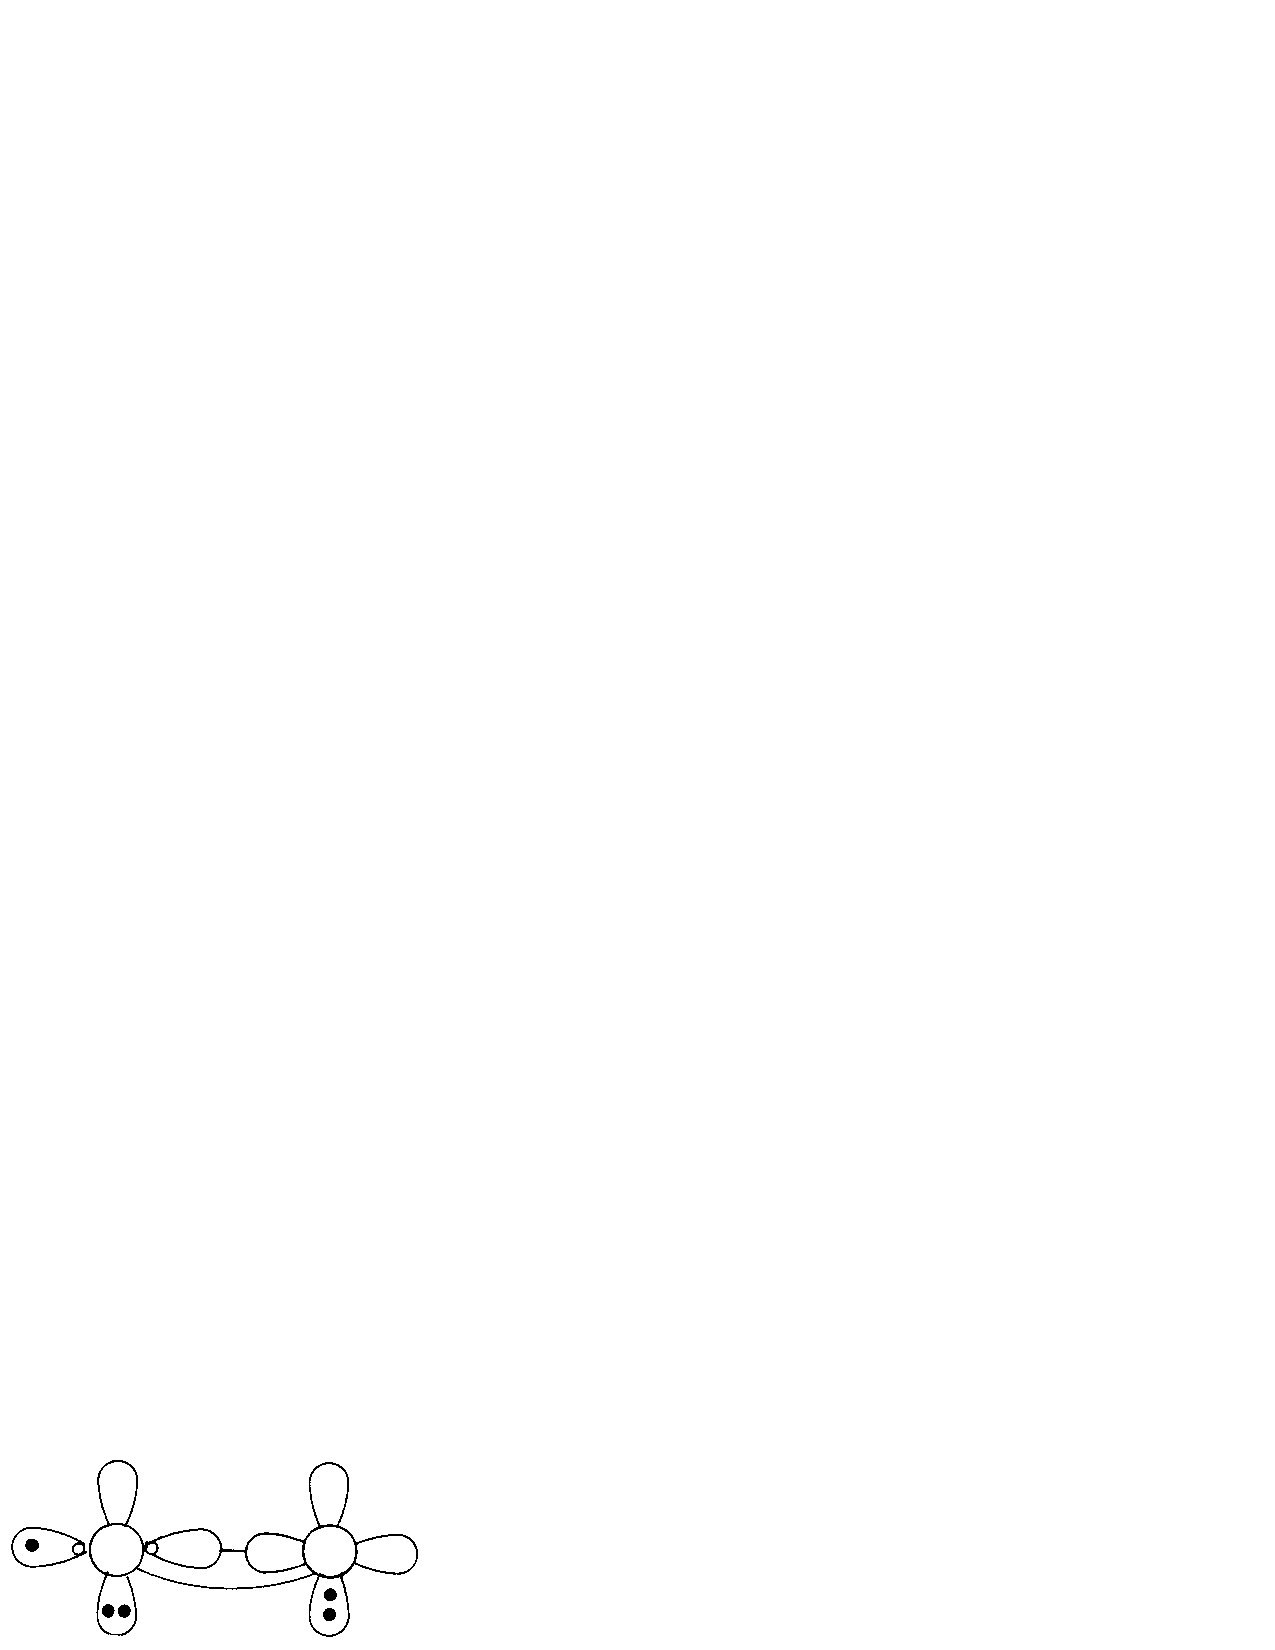
\includegraphics{fg13-7g}
\label{chap13-eqno16}
\end{equation}
leading to $^2\Delta$ and $^2\Sigma^+$ states, and
\begin{equation}
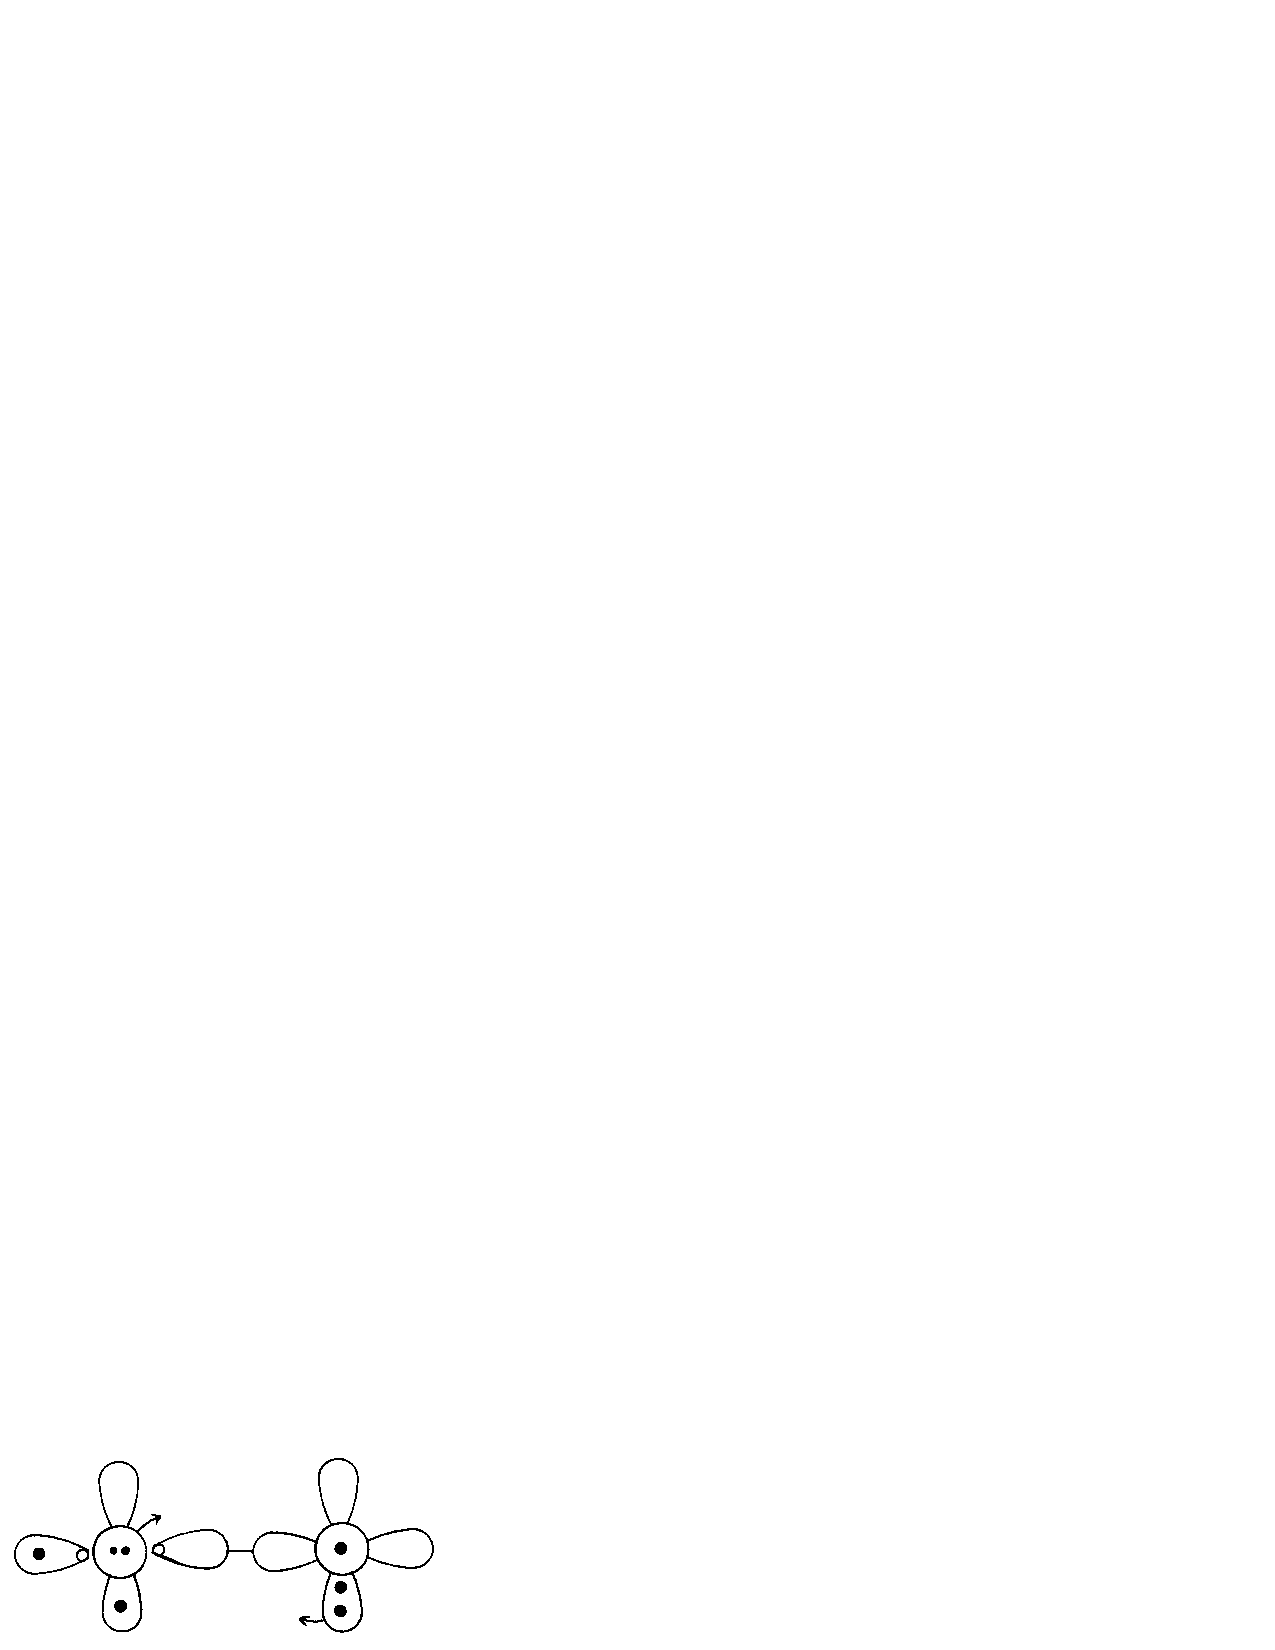
\includegraphics{fg13-7h}
\label{chap13-eqno17}
\end{equation}
leading to $^4\Sigma^-$ and $^2\Sigma^-$, and the other component of 
$^2\Delta$.  States can also be made from O($^1$S)
\begin{equation}
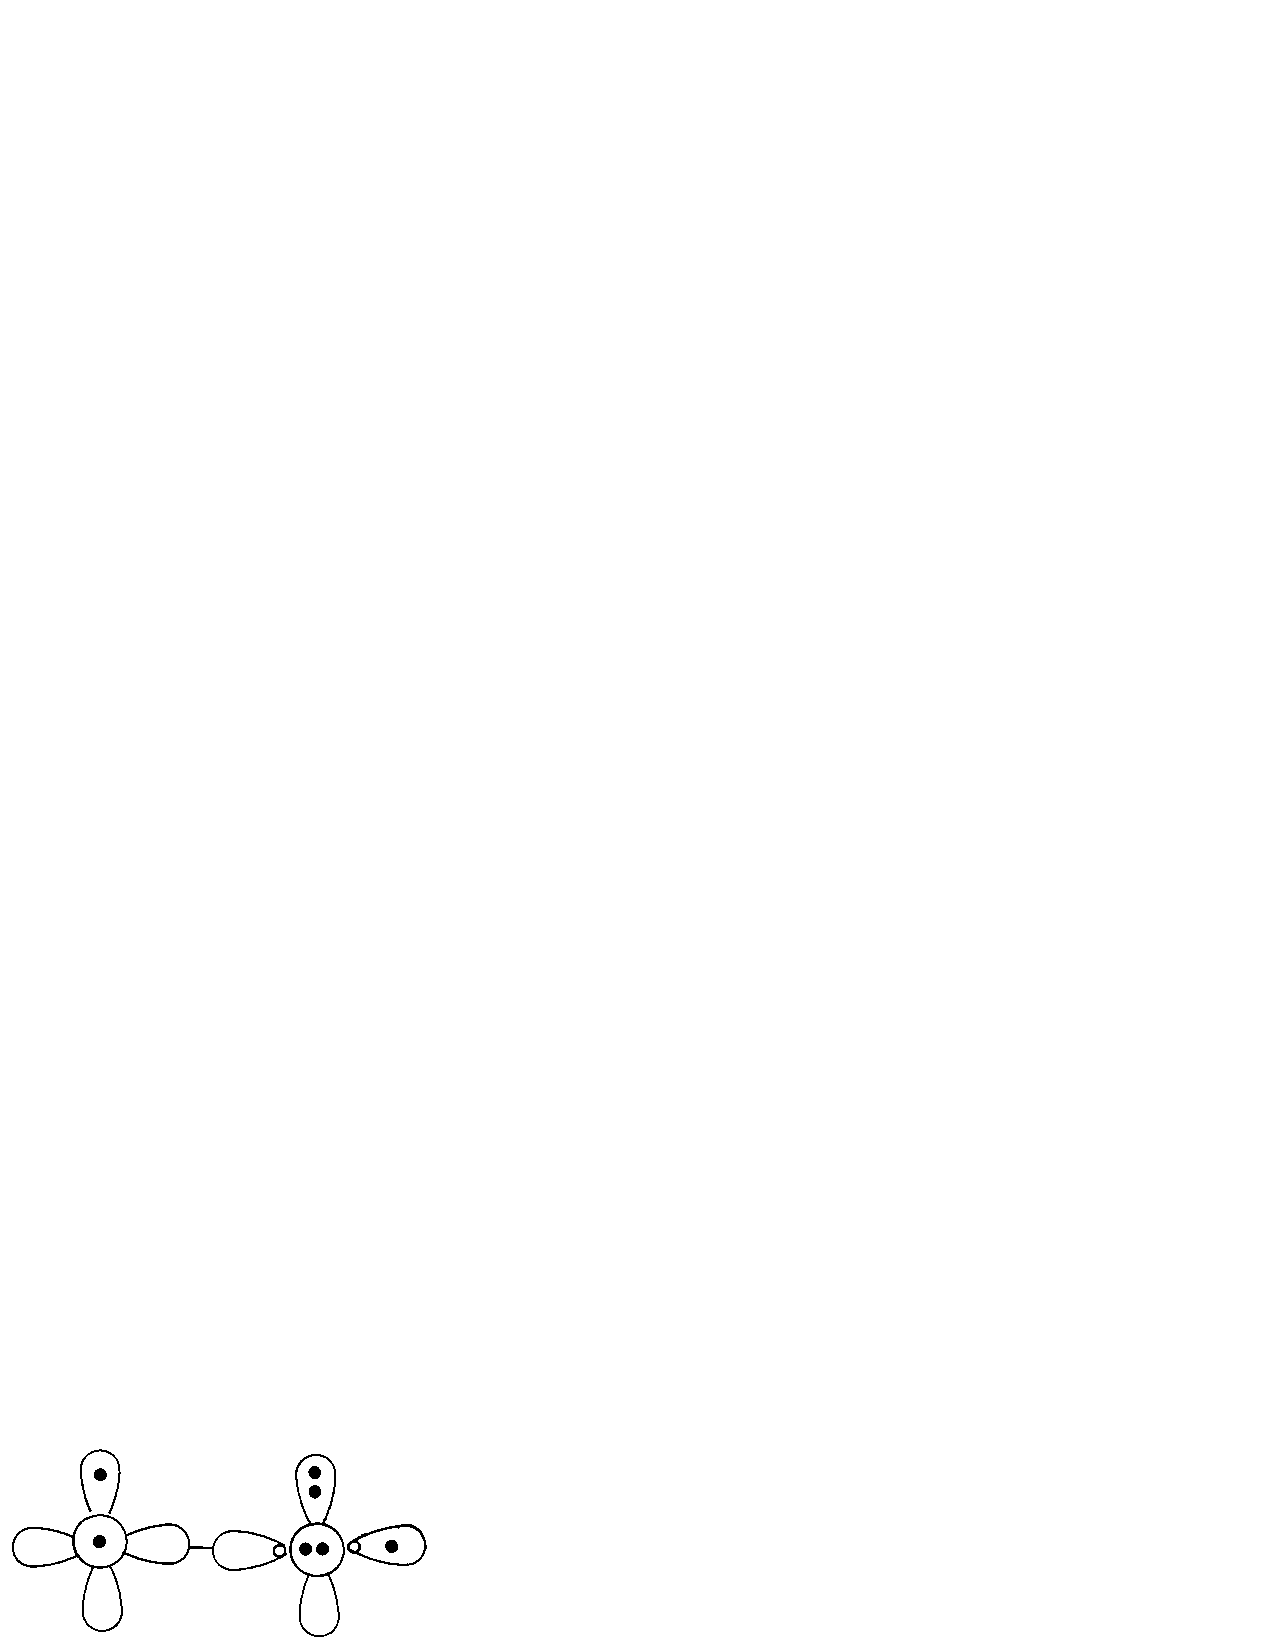
\includegraphics{fg13-7i}
\label{chap13-eqno18}
\end{equation}
leading to $^4\Sigma^-$ and $^2\Sigma^-$.  There is only fragmentary
evidence for most of these states.  Table \ref{chap13-tab8} contains
spectroscopic data on these states, and Figure \ref{chap13-fig7}
contains an energy level diagram.

\begin{table}
\caption{Spectroscopic data for NO.}
\label{chap13-tab8}
\begin{tabular}{ccccc}\\ \hline
& & $T_e$ & $r_e$ & $\omega_e$\cr
& & (cm$^{-1}$) & (\AA) & (cm$^{-1}$)\cr

NO & X $^2\Pi_{12}$ & 121 & 1.1508 & 1904.03\cr
& $^2\Pi_{32}$ & 121 & & 1903.68\cr
& B $^2\Pi_{12}$ & 45919.5 & 1.449$^a$ & 1036.9\cr
& $^2\Pi_{32}$ & 60364.2 & 1.302 & 1217.4\cr
& G $^2\Sigma$ & 0 & 1.3426 & 1085.5\cr
& Rydberg & & 1.1067 & 2377\cr
NO$^+$ & X $^1\Sigma$ & 0 & 1.0619 & 2377.1\cr
& A $^1\Pi$ & 73469.6 & 1.1926 & 1608.9\cr
\hline
\end{tabular}\\
$^a$ Note the large change in $r_e$ for what are presumably two spin-orbital
components of the same $^2\Pi$ state.
\end{table}

\subsection{HNO}

Adding an H to NO, leads to
\begin{equation}
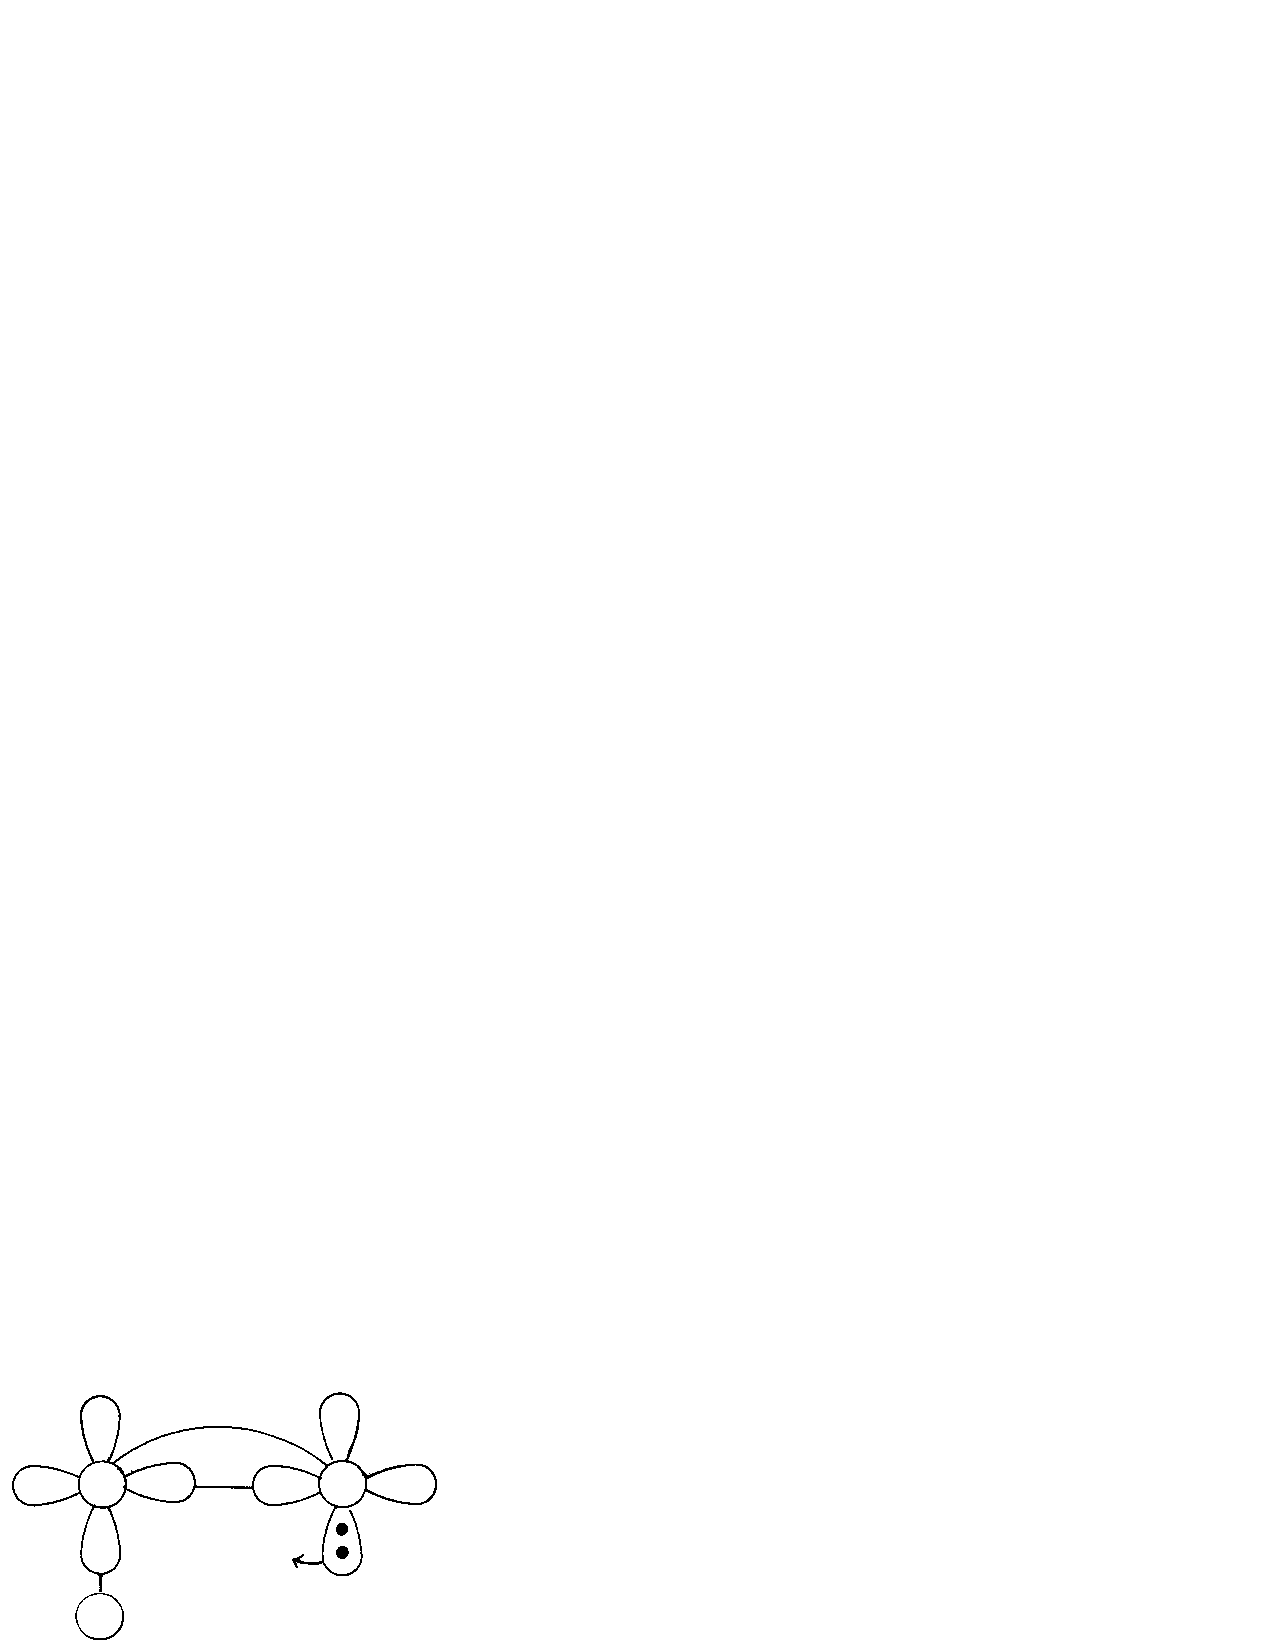
\includegraphics{fg13-7j}
\end{equation}

Because of the overlapping between orbitals in the HN and NO bonds,
the bond angle should increase.  In addition, the interaction with the
O$\pi_x$ pair leads to a further increase.  The result is a bond angle
of 108 degrees.  See Table \ref{chap13-tab9} for data for HNO.

\begin{table}
\caption{Spectroscopic data for HNO.}
\label{chap13-tab9}
\begin{tabular}{ccccccccc}\\ \hline
& & $T_0$ & $r_{HN}$ & $r_{NO}$ & & $\nu_{HN}$ & $\nu_{bond}$ & 
$\nu_{NO}$\cr
& & (cm$^{-1}$) \cr

HNO & (X) $^1A^{\prime}$ & & 1.003 & 1.212 & 108.6 & 3596 & 1562 & 
1110\cr
& $^1A^{\prime \prime}$ & 13154.4 & 1.036 & 1.241 & 116.3 & 2854 & 
1420 & 981\cr
NO & X $^2\Pi$ & & & 1.151 & & & & 1904\cr
\hline
\end{tabular}\\
$^a$D(H-NO) $\leq$ 2.11 eV. 
\end{table}

Because of the bad interaction between the O$\pi_x$ pair and the HN bond, we
might consider
\begin{equation}
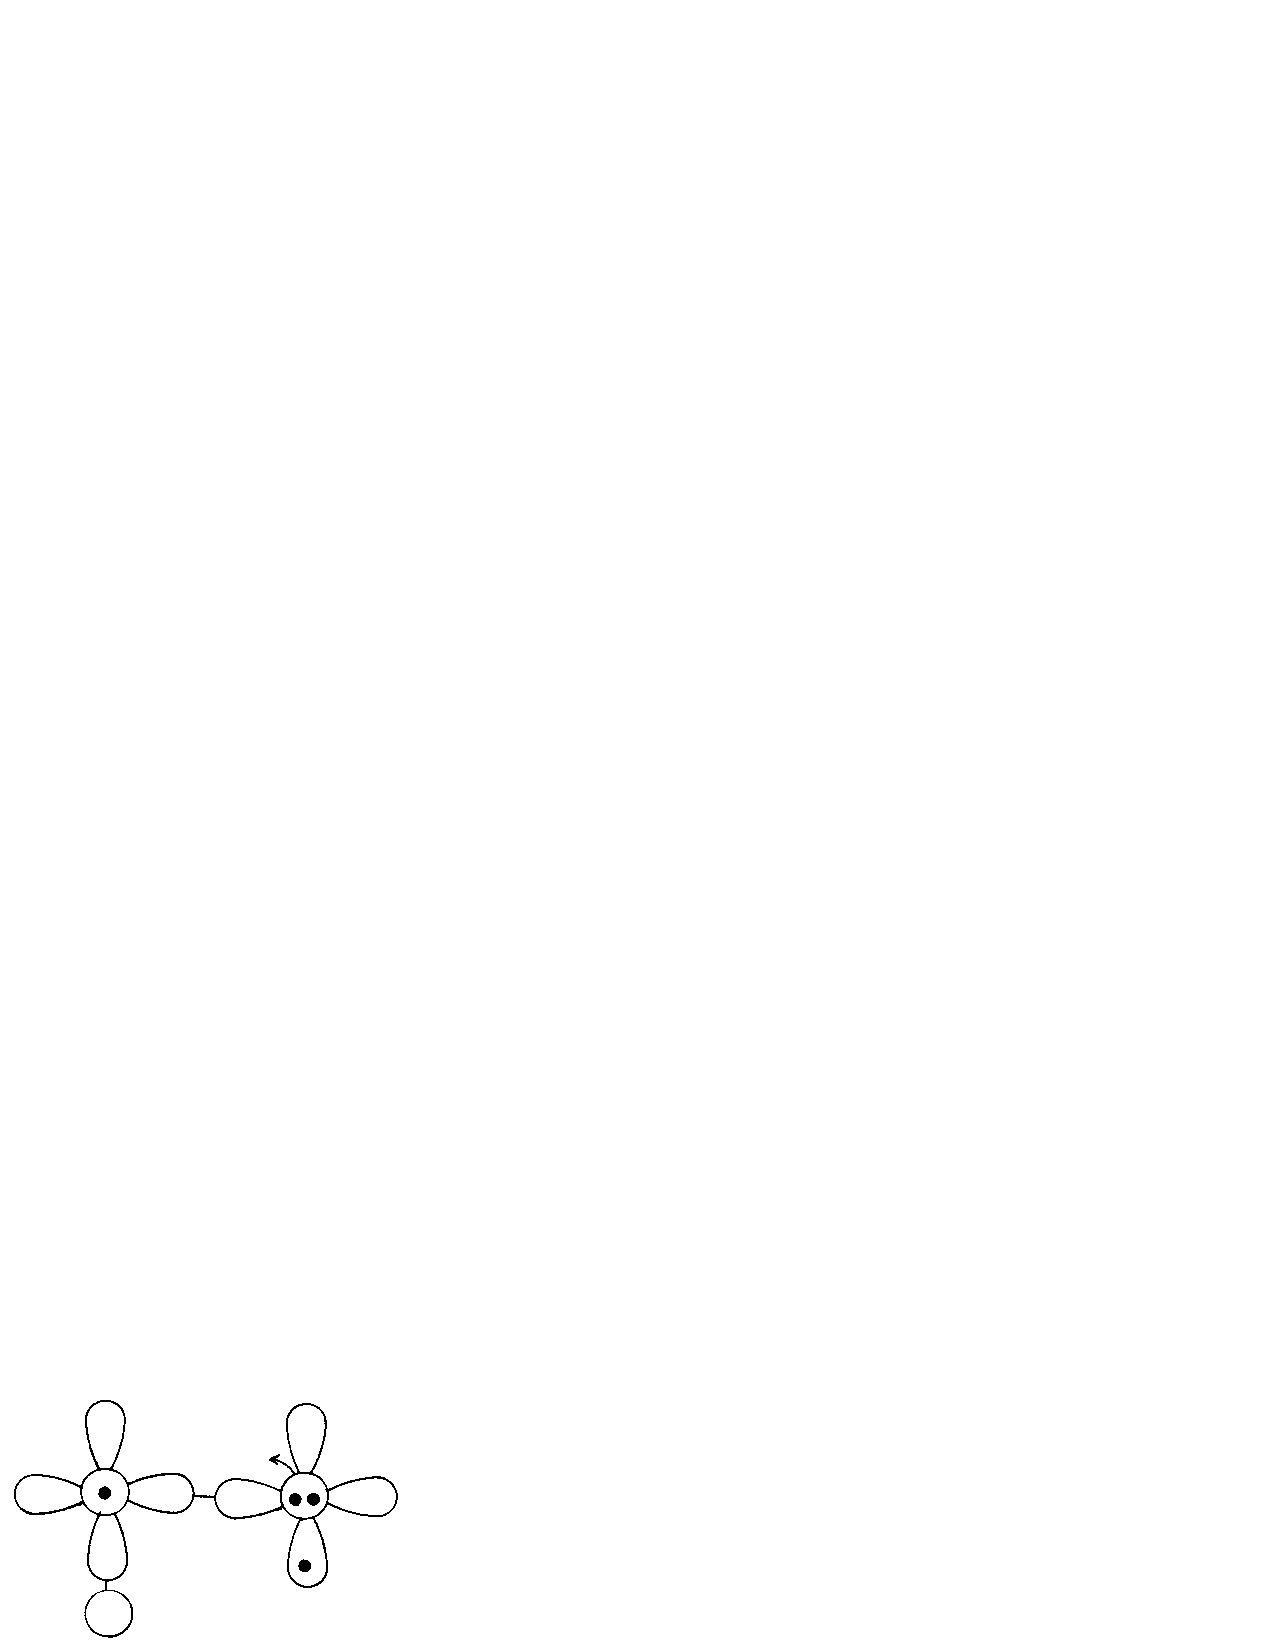
\includegraphics{fg13-7k}
\label{chap13-eqno19}
\end{equation}
This leads to ${^3A}^{\prime \prime}$ and ${^1A}^{\prime \prime}$
states, and should account for the excited state in Table
\ref{chap13-tab9}.  However, we would not expect the bond angle of
(\ref{chap13-eqno19}) to increase as it does to 110 degrees.

\subsection{NCO and H$_2$O}

The bonding in the ground state of NCO should be
\begin{equation}
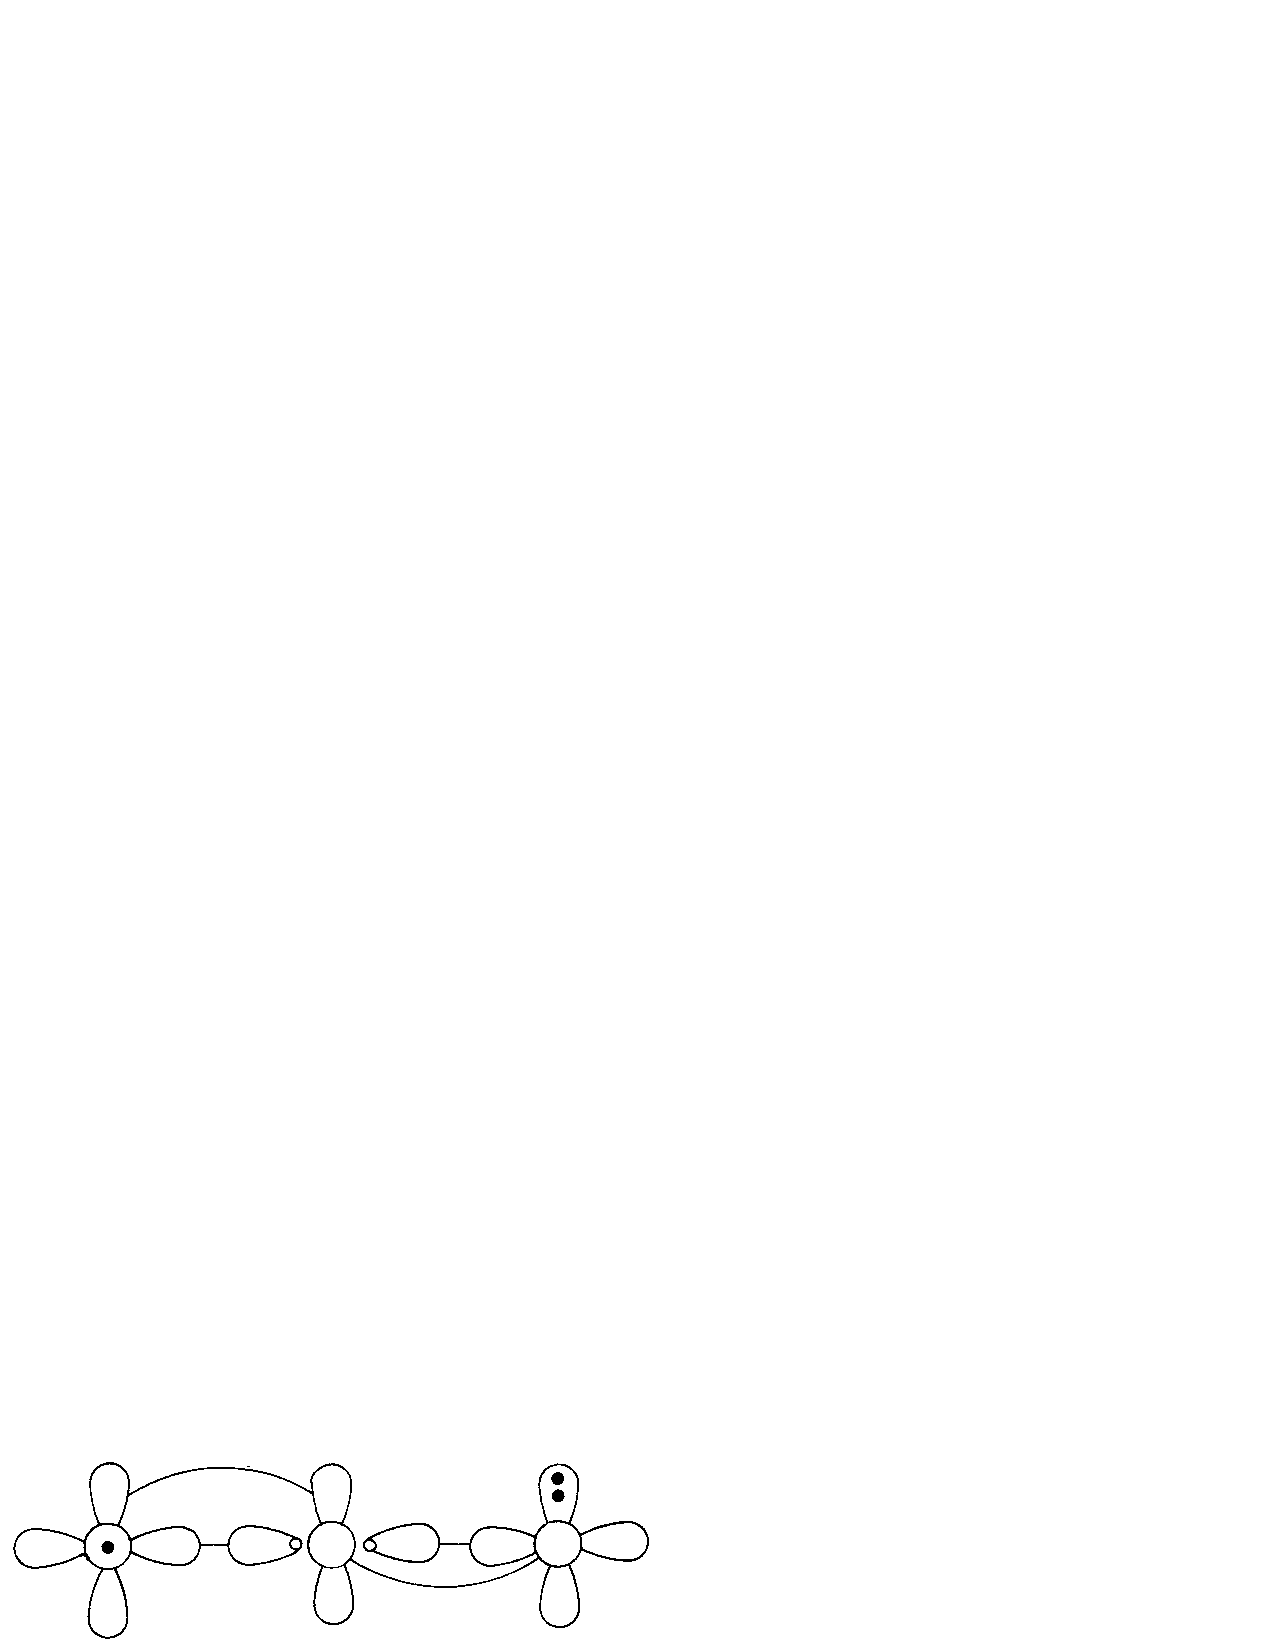
\includegraphics{fg13-7l}
\end{equation}
leading to a linear $^2\Pi$ state.

The best bonding for N$_2$O would appear to be
\begin{equation}
\includegraphics{fg13-7m}
\end{equation}
leading to a $^1\Sigma^+$ analogous to that of CO$_2$.

\subsection{NO$_2$}

Starting with NO and O, we obtain
\begin{equation}
\includegraphics{fg13-7n}
\end{equation}
and
\begin{equation}
\includegraphics{fg13-7o}
\end{equation}
as possible states of NO$_2$.  Exciting the N(2s) in
(\ref{chap13-eqno17}), we also obtain
\begin{equation}
\includegraphics{fg13-7p}
\end{equation}

Configuration (\ref{chap13-eqno16}) leads to $^2A_1$, lower, and
$^2B_2$ states, while (\ref{chap13-eqno17}) leads to $^2A_2$, lower,
and $^2B_1$ states.  In addition, (\ref{chap13-eqno18}) leads to a
$^2A_1$ state.  But the $^2A_1$ states obtained from
(\ref{chap13-eqno16}) and (\ref{chap13-eqno18}) should mix very
strongly, leading to a low-lying $^2A_1$ state, as observed, see Table
\ref{chap13-tab10}.

Note quartet states can be obtained from a modification of
(\ref{chap13-eqno18})
\begin{equation}
\includegraphics{fg13-7q}
\end{equation}
leading to
\begin{equation}
\includegraphics{fg13-7r}
\end{equation}
having $^4B_2$ symmetry, and
\begin{equation}
\includegraphics{fg13-7s}
\end{equation}
having $^2B_2$ symmetry.

\begin{table}
\caption{Spectroscopic data for NO$_2$.}
\label{chap13-tab10}
\begin{tabular}{cccc}\\ \hline
& & $r_{NO}$ & ONO\cr

X$^2A_1$ & 0 & 1.1934 & 134.1\cr
A($^2B_1$) & $<$15000\cr
B$^2B_2$ & 40125.9 & 1.314 & 121.0\cr
C & (42500)\cr
D & (50000)\cr
E$^2\Sigma^+_u$ & (58309) & 1.1$^3$ & 180$^{\circ}$\cr
\hline
\end{tabular}\\
IP = 9.78 and D(ON=O) = 3.114$^9$.
\end{table}

